% ------------------------------------------------------------------------
%
% -------------------      Plantilla_UIS.tex       -----------------------
%
% ------------------------------------------------------------------------
% ------------------------------------------------------------------------
% ------------------------------------------------------------------------
% Versión de plantilla para realización de informes de trabajo de grado
% construida para uso de la Universidad Industrial de Santander.
%
% Reservados todos los derechos
%
% Bucaramanga, Colombia
%
% Septiembre 17 de 2018
%

\documentclass[letter,oneside,12pt,spanish]{report}          % Encabezados
% ------------------------------------------------------------------------
\usepackage{uislatexstyleICONTEC}                   % Libreria UIS ICONTEC
% ------------------------------------------------------------------------
% Ingrese en este punto las librerías específicas de usuario
% ------------------------------------------------------------------------
%\usepackage{epsfig}
%\usepackage{amssymb}
\usepackage{subfigure}
\usepackage{float}
\usepackage{siunitx}
\usepackage{multirow}
% ------------------------------------------------------------------------
% Archivo de bibliografía
% ------------------------------------------------------------------------
%\addbibresource{reference.bib}
% ------------------------------------------------------------------------

\usepackage{fourier}%soul
%\usepackage{calc}
%\usepackage{minitoc}
\usepackage{tikz}
%\usepackage{lipsum}
\usepackage{color}
\definecolor{escuela}{RGB}{201,149,0}
\definecolor{uis}{RGB}{103,185,62}
\definecolor{Nb}{RGB}{76,178,118}
\definecolor{Ta}{RGB}{183,154,86}
\definecolor{Sr}{RGB}{0,255,38}
\definecolor{O}{RGB}{254,3,0}
\definecolor{N}{RGB}{176,185,230}


\begin{document}                                     % Inicio de documento
% ------------------------------------------------------------------------
% Definición silábica de palabras
% ------------------------------------------------------------------------
\hyphenation{pro-por-cio-nal di-se-ño}
% ------------------------------------------------------------------------
% Elementos previos al contenido del trabajo
% ------------------------------------------------------------------------
% ------------------------------------------------------------------------
%                                 Portada
% ------------------------------------------------------------------------

\thispagestyle{empty}

\begin{center}

INVESTIGACIÓN TEÓRICA DE LAS ESTRUCTURAS RUDDLESDEN-POPPER DE LOS OXINITRUROS $Sr_{2}(Ta,Nb)O_{4-x}N_{x}$($x=0.5$ Y $1.0$) A TRAVÉS DE LA TEORÍA FUNCIONAL DE LA DENSIDAD \vspace{6.83cm}

JUAN ALEJANDRO PINTO CASTRO\\
\vspace{6.83cm}

UNIVERSIDAD INDUSTRIAL DE SANTANDER\\
FACULTAD DE CIENCIAS BÁSICAS\\
ESCUELA DE FÍSICA\\
FÍSICA COMPUTACIONAL EN MATERIA CONDENSADA\\
BUCARAMANGA\\
2021\\

\end{center}

% ------------------------------------------------------------------------
%                              Contraportada
% ------------------------------------------------------------------------

\newpage
\thispagestyle{empty}

\begin{center}

INVESTIGACIÓN TEÓRICA DE LAS ESTRUCTURAS RUDDLESDEN-POPPER DE LOS OXINITRUROS $Sr_{2}(Ta,Nb)O_{4-x}N_{x}$($x=0.5$ Y $1.0$) A TRAVÉS DE LA TEORÍA FUNCIONAL DE LA DENSIDAD \vspace{2.85cm}

JUAN ALEJANDRO PINTO CASTRO\\
\vspace{2.15cm}

Trabajo de Grado para optar al título de\\
Físico\\\vspace{2.35cm}

Director\\
Andrés Camilo García Castro\\
Doctorado en Física \vspace{2.35cm}

UNIVERSIDAD INDUSTRIAL DE SANTANDER\\
FACULTAD DE CIENCIAS BÁSICAS\\
ESCUELA DE FÍSICA\\
FÍSICA COMPUTACIONAL EN MATERIA CONDENSADA\\
BUCARAMANGA\\
2021\\

\end{center}

% ------------------------------------------------------------------------
%                             Nota de proyecto
% ------------------------------------------------------------------------

\newpage
\pagenumbering{arabic} \setcounter{page}{3}

%\begin{figure}
%\begin{center}
%\includegraphics[width=1.0\textwidth]{Figs/nota}
%\end{center}
%\end{figure}

% ------------------------------------------------------------------------
%                             Autorización
% ------------------------------------------------------------------------

\newpage

%\begin{figure}
%\begin{center}
%\includegraphics[width=0.9\textwidth]{Figs/autoriza.eps}
%\end{center}
%\end{figure} 
% ------------------------------------------------------------------------   % Portada, contraportada, formato de nota y autorización
% ------------------------------------------------------------------------
% ------------------------------------------------------------------------
% ------------------------------------------------------------------------
% ------------------------------------------------------------------------
%                               Dedicatoria
% ------------------------------------------------------------------------
% ------------------------------------------------------------------------
% ------------------------------------------------------------------------
\chapter*{}%DEDICATORIA}

\begin{flushright}
A\\
\textit{Mi madre y mi padre}
%Este trabajo viene dedicado para todas aquellas personas que apoyaron el desarrollo y ejecución de este trabajo de grado.\\

%En especial reconozco la permanente presencia de Dios en mi camino de vida. 
\end{flushright}

% ------------------------------------------------------------------------                                      % Dedicatoria
% ------------------------------------------------------------------------
% ------------------------------------------------------------------------
% ------------------------------------------------------------------------
% ------------------------------------------------------------------------
%                             AGRADECIMIENTOS
% ------------------------------------------------------------------------
% ------------------------------------------------------------------------
% ------------------------------------------------------------------------
\chapter*{AGRADECIMIENTOS}

Expreso mis agradecimientos a las personas que me acompañaron durante el desarrollo de este trabajo de investigación en física y materia condensada:\\

Ph.D. Andrés Camilo García Castro

Director del trabajo de investigación en pregrado.\\

Ph.D. Ilia Davidovich Mikhailov

Profesor que otorgó las bases de mi conocimiento.\\

A todos mis compañeros de carrera que junto a una taza de café debatíamos nuestros pensamientos académicos, científıcos y culturales, ellos son:\\

Juan Sebastián Gelves Badillo

Jhonatan Mackalister Durán Pinilla

Luis Gabriel Mesa Suárez

Holger Giovani Quintero Santander\\

Agradezco a mi familia por el apoyo económico y moral que tuvieron para conmigo durante el desarrollo de mi carrera.\\
% ------------------------------------------------------------------------
\newpage                              % Agradecimientos
% ------------------------------------------------------------------------
\tableofcontents                                      % Tabla de contenido
% ------------------------------------------------------------------------
\listoffigures                         % Lista de figuras, tablas y anexos
\listoftables
\listofanexo
% ------------------------------------------------------------------------
% ------------------------------------------------------------------------
% ------------------------------------------------------------------------
% ------------------------------------------------------------------------
%                                Glosario
% ------------------------------------------------------------------------
% ------------------------------------------------------------------------
% ------------------------------------------------------------------------
\chapter*{LISTA DE ACRÓNIMOS}

\begin{description}
  \item[RP] Ruddlesden-Popper
  \item[DFT] Density Functional Theory
  \item[DFT+U] Density Functional Theory + Hubbard-like Term
  \item[SOD] Site Ocupanccy Disorder
  \item[LDA] Local Density Aproximation
  \item[GGA] Generalised Gradient Aproximation
  \item[PBEsol] Perdew-Burke-Ernzenhof revised for solids
  \item[VASP] Vienna Ab-initio Simulation Package
\end{description}

% ------------------------------------------------------------------------                                % Glosario de términos
% ------------------------------------------------------------------------
% Contenido del Informe
% ------------------------------------------------------------------------
% ------------------------------------------------------------------------
% ------------------------------------------------------------------------
% ------------------------------------------------------------------------
%                                Resumen
% ------------------------------------------------------------------------
% ------------------------------------------------------------------------
% ------------------------------------------------------------------------
\chapter*{RESUMEN}

\footnotesize{
\begin{description}
  \item[TÍTULO:] INVESTIGACIÓN TEÓRICA DE LAS ESTRUCTURAS RUDDLESDEN-POPPER DE LOS OXINITRUROS $Sr_{2}(Ta,Nb)O_{4-x}N_{x}$($x=0.5$ Y $1.0$) A TRAVÉS DE LA TEORÍA FUNCIONAL DE LA DENSIDAD\astfootnote{Trabajo de grado}
  \item[AUTOR:] JUAN ALEJANDRO PINTO CASTRO\asttfootnote{Facultad de Ciencias Básicas. Escuela de Física, Física computacional en Materia Condensada. Director: Andrés Camilo García Castro, Doctorado en Física.}
  \item[PALABRAS CLAVE:] PEROVSKITA, RUDDLESDEN-POPPER, TEORÍA FUNCIONAL DE LA DENSIDAD, FERROELECTRICIDAD, FOTOCATÁLISIS.
  \item[DESCRIPCIÓN:]\hfill \\ La fase Ruddlesden-Popper (\textsc{rp}) es un tipo de perovskita dispuesta en capas dislocadas, considerada como un intercrecimiento de $n$ capas de perovskita $ABX_{3}$ y una capa $AX$: $(AX)(ABX_{3})$. 
  La sustitución parcial de oxígeno, O$^{2-}$, por nitrógeno, N$^{3-}$, en óxidos metálicos (basados en sus similitudes en electronegatividad, polarizabilidad, radio iónico y número de coordinación) conlleva a  modificaciones de sus propiedades físicas asociadas a respuestas eléctricas, ópticas, catalíticas y magnéticas. Adicioalmente, se prevee un posible comportamiento ferroeléctrico inducido por esta sustitución. 
  En el actual trabajo se presenta el análisis teorico de las propiedades estructurales, electrónicas y fonónicas del compuesto $Sr_{2}(Ta,Nb)O_{4-x}N_{x}$ para dos concentraciones aniónicas $x=0.5$ y $x=1.0$. El anteior analisis logrado mediante el uso de teoría funcional de la densidad, DFT, implementada en el paquete de simulación Vienna ab initio (\textsc{vasp}) compilado en el cluster \texttt{"Guane"} de la supercomputadora de la Universidad industrial de Santander (\textsc{uis}).
  
  En detalle, con el fin de cubrir un completo ensamble de combinaciones anionicas posibles, se realizó la sustitución aniónica a traves del código \textsc{sod} obteniendo 11 configuraciones con concentración $x=1$, y dos configuraciones con concentración $x=0.5$, todas con diferente orden aniónico. 
  Posteriormente se realizó la relajación estructural, encontrando dos configuraciones de mínima energía con ordenamiento aniónico \emph{trans} y \emph{cis}, pertenecientes al grupo espacial $Immm(71)$ y $Cmcm(63)$, respectivamente. 
  Cálculos de \textsc{dft} indican que el orden aniónico \emph{cis} es energéticamente más favorable que el orden aniónico \emph{trans}. 
  La estructura electrónica sugiere un material aislante con una reducción del bandgap en el punto $\Gamma$ de la zona de Brillouin debido a la introducción del nitrógeno en la estructura, permitiendo el uso de luz en el rango visible para la división de agua mediante fotocatálisis. 
  La estructura fonónica evidencia modos imaginarios que llevan a desplazamientos del metal de transición, y por ende una caída de la simetría espacial, logrando una transición de fase al más favorable modo suave quiral perteneciente al grupo espacial $C222_{1}$ (SG. 20).

\end{description}}\normalsize
% ------------------------------------------------------------------------                                                % Resumen
% ------------------------------------------------------------------------
% ------------------------------------------------------------------------
% ------------------------------------------------------------------------
%                                Abstract
% ------------------------------------------------------------------------
% ------------------------------------------------------------------------
% ------------------------------------------------------------------------
\chapter*{ABSTRACT}

\footnotesize{
\begin{description}
  \item[TITLE:] THEORETICAL INVESTIGATION OF THE RRUDLESDEN-POPPER OXINITRIDES STRUCTURES\\ $Sr_{2}(Ta,Nb)O_{4-x}N_{x}$ VIA DENSITY FUNCTIONAL THEORY \astfootnote{B. Sc. Thesis}
  \item[AUTHOR:] JUAN ALEJANDRO PINTO CASTRO\asttfootnote{Faculty of Sciences. School of Physics. Advisor: Andrés Camilo García Castro, Ph.D in Physics.}
  \item[KEYWORDS:] PEROVKSITE, RRUDLESDEN-POPPER, DENSITY FUNCTIONAL THEORY, FERROELECTRICITY \& PHOTOCATALYSIS.
  \item[DESCRIPTION:]\hfill \\ Ruddlesden-Popper phase (\textsc{rp}) is a type of perovskite arranged in dislocated layers, considered as an intergrowth of $n$  layers of perovskite $ABX_{3}$ and a layer $AX$:$(AX)(ABX_{3})$.
  The partial replacement of oxygen, $O^{2-}$, by nitrogen, $N^{3-}$, in metal oxides (based on their similarities in electronegativity, polarizability, ionic radius, and coordination number) entails a modification of its physical properties associated with electrical, optical, catalytic and magnetic responses. Additionally, a possible ferroelectric behavior induced by this substitution is anticipated.
  The current work presents the theoretical analysis of the structural, electronic and phononic properties of the compound $Sr_{2}(Ta,Nb)O_{4-x}N_{x}$ for two anionic concentrations $x=0.5$ y $x=1.0$. The previous analysis was achieved through the use of density functional theory, \textsc{dft}, implemented in the Vienna ab initio simulation package (\textsc{vasp}) compiled in the \texttt{"Guane"} cluster of the University supercomputer Santander industrial (\textsc{uis}).
  
  In detail, in order to cover a complete assembly of possible anionic combinations, the anionic substitution was operated through the code \textsc{sod} obtaining 11 configurations with concentration $x=1.0$, and two configurations with concentration $x=0.5$, all with different anion order.
  Subsequently, the structural relaxation was carried out, finding two configurations of minimum energy with anionic ordering \emph{trans} and \emph{cis}, belonging to the space group $Immm$ (S.G. 71) and $Cmcm$ (S.G. 63), respectively.
  Calculations from \textsc{dft} indicate that the anionic order \emph{cis} is energetically more favorable than the anionic order \emph{trans}.
  The electronic structure suggests an insulating material with a reduction of the bandgap in the point $\Gamma$ of the Brillouin zone due to the introduction of nitrogen in the structure, allowing the use of light in the visible range for the division of water by photocatalysis.
  The phononic structure shows imaginary modes that lead to displacement of the transition metal, and therefore a drop in spatial symmetry, achieving a phase transition to the most favorable chiral smooth mode belonging to the space group $C222_ {1}$ (SG. 20). 
\end{description}}\normalsize
% ------------------------------------------------------------------------                                               % Abstract
% ------------------------------------------------------------------------
% Capítulos
% ------------------------------------------------------------------------
% ------------------------------------------------------------------------
% ------------------------------------------------------------------------
% ------------------------------------------------------------------------
%                              Introducción
% ------------------------------------------------------------------------
% ------------------------------------------------------------------------
% ------------------------------------------------------------------------

\nnchapter{INTRODUCCIÓN}
% ------------------------------------------------------------------------
% ------------------------------------------------------------------------
Los cerámicos con estructura cristalográfica tipo perovskita han sido parte fundamental de la ciencia y tecnología gracias a la variedad de propiedades físicas que pueden llegar a adquirir \cite{Howard2005StructuresApproach,Sarmiento-Perez2015PredictionPerovskites}. Los acoplamientos y alteraciones que se han realizado desde el descubrimiento del mineral titanato de calcio ($CaTiO_{3}$), también conocido como perovskita, han sido esenciales para encontrar nuevas propiedades magnéticas y eléctricas, consiguiendo materiales aislantes\cite{Tokura1997Metal-insulatorOxide}, conductores\cite{Chen2017Atomic-ScaleStructures}, semiconductores\cite{Garcia-Esparza2019FullFuels} y superconductores\cite{Maeno1994SuperconductivityCopper}, hasta materiales multiferroicos\cite{Cruz2014PiezoelectricThickness}, magnetoeléctricos\cite{Fiebig2005RevivalEffect} y materiales multiferróicos magnetoeléctricos\cite{Hill2000WhyFerroelectrics}. La versatilidad de la perovskita cúbica $ABX_{3}$ permite distintas posibilidades de agrupación, consiguiendo sistemas laminares, los cuales son formados por capas que crecen en una dirección específica, como la perovskita doble, Dion-Jacobson, Ruddlesden-Popper y Aurivillus \cite{Benedek2015Undestanding}.

\begin{figure}[h!]
    \centering
    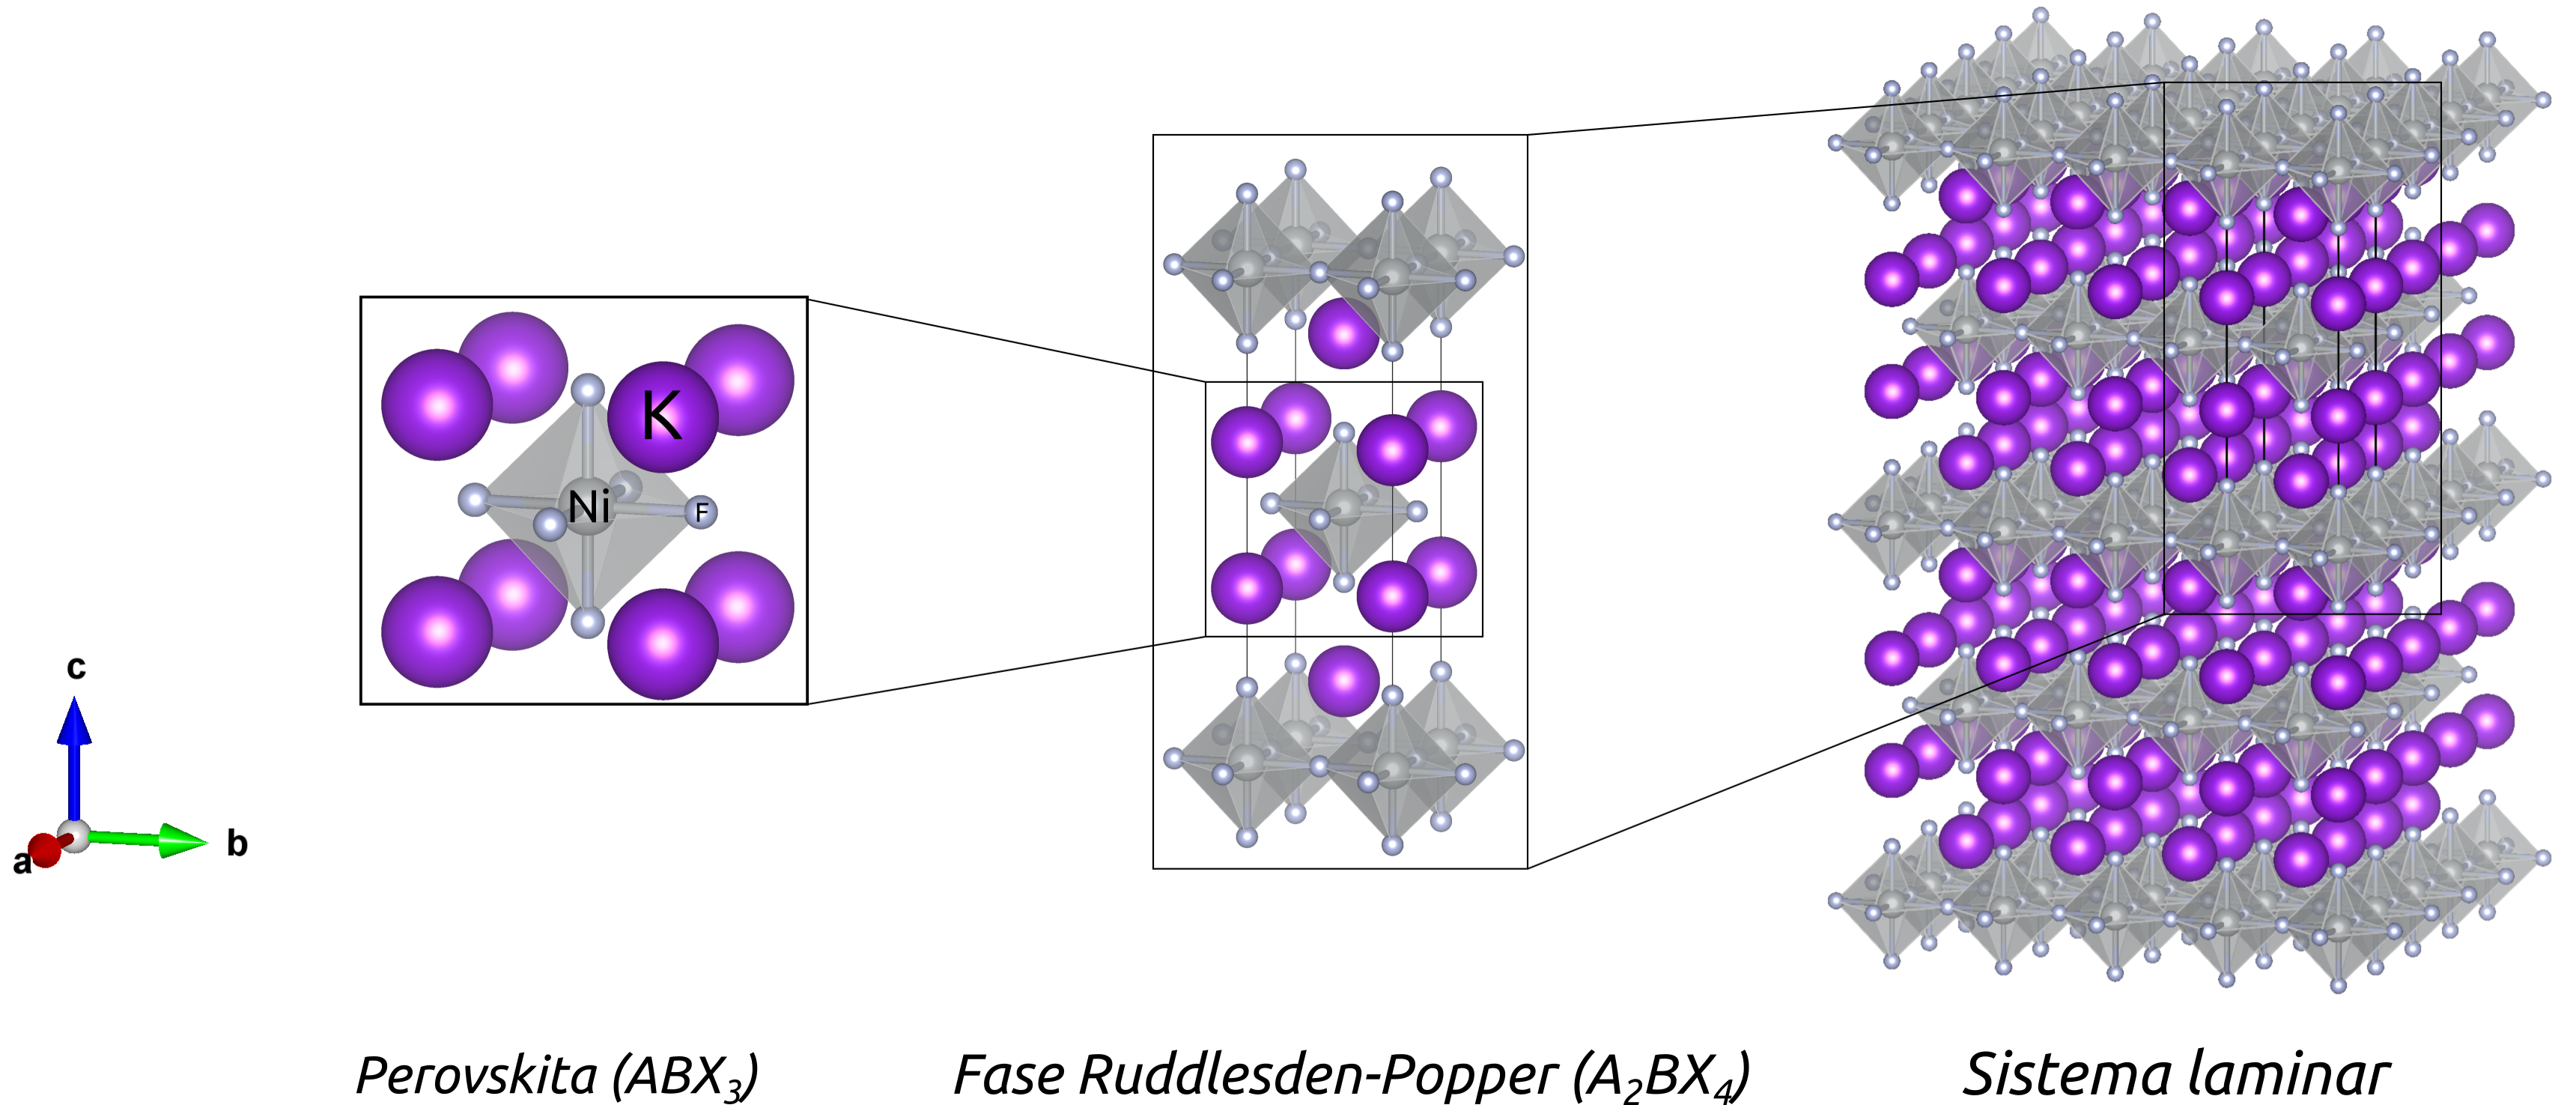
\includegraphics[width=13.0cm,keepaspectratio=true]{Figs/material1.png}
    \caption{Estructura $K_{2}NiF_{4}$ de la familia de estructuras tipo Ruddlesden-Popper \cite{NRuddl1957NewType}.}
    \label{fig:k2nif4}
\end{figure}

La figura \ref{fig:k2nif4} muestra un sistema laminar de perovskitas distribuidas por capas dislocadas formando la familia de estructuras Ruddlesden-Popper, la cual se descubrió en el material $K_{2}NiF_{4}$. Algunos ejemplos son: $Sr_{2}TiO_{4}$, $Ca_{2}MnO_{4}$ y $Sr_{2}LaAlO_{4}$ \cite{NRuddl1957NewType}. La familia \textsc{rp} se distingue por su formula química $A_{n+1}B_{n}X_{3n+1}$, donde $n$ indica la fase de la estructura dentro de la familia \textsc{rp} \cite{Fuertes2012ChemistryPerovskites}. En el presente trabajo, la fase considerada es $n=1$ que lleva a la fórmula química $A_{2}BX_{4}$, donde los átomos $A$ y $B$ son cationes y los átomos $X$ son aniones \cite{Clarke2002}. Esta fase \textsc{rp} es formada si los sitios cristalográficos $A$ son ocupados por cationes más grandes, indicando que deben tener valencias de $1+$ o $2+$ \cite{Beznosikov2000}, como es el caso del estroncio ($Sr^{2+}$) al disponerlo en la celda unitaria. De esta manera, la fase \textsc{rp} toma la forma $Sr_{2}BX_{4}$. Este proyecto se enfoca en dos materiales con diferente metal de transición: tántalo y niobio $(Ta,Nb)$, ocupando el sitio cristalográfico $B$, ya que estos cationes al combinarlos con nitrógeno pasarán de una oxidación $4+$ a una oxidación $5+$, lo cual hace a la estructura mas estable, como ocurre en el caso de la perovskita $SrNbO_{2}N$ \cite{Tobias2004}. El átomo de oxigeno ocupa el sitio $X$ dando la forma a la estructura $Sr_{2}(Ta,Nb)O_{4}$. El enfoque que se le da a esta estructura consiste en la variación de la concentración de oxígeno, sustituyendo estos aniones por átomos nitrógeno, dando lugar a la estructura oxinitrada $Sr_{2}(Ta,Nb)O_{4-x}N_{x}$, para encontrar nuevas estructuras cristalográficas que exhiben propiedades como fotocatálisis para división de agua y comportamiento  ferroeléctricos debido a la dependencia del ordenamiento aniónico
\cite{Bouri2018,Morgan1986,Page2007LocalTheory}.

La perovskita tipo Ruddlesden-Popper ha atraído la atención como un posible nuevo material ferroeléctrico debido al orden aniónico en la estructura cristalina \cite{Gou2020Photocatalysis}. Se han reportado oxinitruros de metales de transición sensibles al orden de óxido-nitruro, alterando las propiedades ópticas, foto-catalíticas, dieléctricas y magnetorresistivas, además de ser más estables en el aire y la humedad que los nitruros puros\cite{Yang2011}. Los oxinitruros a menudo exhiben colores brillantes y una resistividad significativamente menor en comparación con los óxidos puros de metales de transición com $Ti^{5+}$, $Nb^{5+}$ o $Ta^{5+}$ \cite{Ebbinghaus2004}. Una forma de obtener oxinitruros a partir de oxidos puros es realizar substituciones atómicas de los sitios cristalográficas para determinar la disposición de los átomos sustituidos en la estructura, a través del código \textit{Site Ocupanccy Disorder} (\textsc{sod}) \cite{Grau-Crespo2007}.

El presente trabajo de grado expone una investigación teórica mediante la teoría funcional de la densidad (\textsc{dft}), basada como su nombre lo indica, es una funcional de la densidad electrónica de todo el sistema. Las funciones de onda se pueden expresar en términos de esta densidad electrónica y resolver la ecuación de Schrödinger simplemente definiendo el funcional de la densidad con solo tres variables espaciales en lugar de $3N$ variables.\cite{ACGarcia2016phd}. Esta investigación teórica permitirá caracterizar el material mediante el análisis de sus propiedades, de su estructura electrónica y estructura fonónica.

El capítulo uno de esta tesis se abordan conceptos fundamentales de perovskitas tipo \textsc{rp}, materiales oxinitrados y sus propiedades. En el componente teórico se incluye la teoría funcional de la densidad (\textsc{dft}), el parámetro \textsc{u} construido en \textsc{dft+u}, además del modelo de aproximación armónica y la corrección no analítica \cite{Wang_2010-nac} implementado en el código \textsc{phonopy} \cite{Togo2015phonopy}, para calcular la dispersión de fonones. En el capitulo dos se realiza un análisis de las sustituciones aniónicas y la relajación estructural de las configuraciones \textsc{rp} encontradas, junto con su caracterización como los parámetros de red, el volumen de la celda y el grupo espacial. Posteriormente en el capítulo tres se discute la estructura electrónica de las configuraciones mas estables energéticamente, además de su posible aplicación en fotocatálisis para división de agua. Luego se analiza la estructura fonónica de las configuraciones mas favorables con ordenamiento aniónico \emph{trans} y \emph{cis} para encontrar fases polares que lleven a una posible ferroelectricidad. Finalmente se presentan las conclusiones, recomendaciones y posibles trabajos futuros conseguidos en el desarrollo de la investigación.



% ------------------------------------------------------------------------
% ------------------------------------------------------------------------ % Introducción
%% ------------------------------------------------------------------------
% ------------------------------------------------------------------------
% ------------------------------------------------------------------------
%                              Objetivos
% ------------------------------------------------------------------------
% ------------------------------------------------------------------------
% ------------------------------------------------------------------------

\chapter*{LISTA DE ACR\'ONIMOS}
\begin{acronym}
\acro{RP}[RP]{Ruddlesden-Popper}
\acro{DFT}[DFT]{Density Functional Theory}% - Teoría Funcional de la Densidad}
\acro{DFT+U}[DFT+U]{Density Functional Theory + Hubbard-like Term}
\acro{SOD}[SOD]{Site Ocupanccy Disorder}% - Desorden de Ocupación de Sitio}
\acro{LSDA}[LSDA]{Local Spin Density Aproximation}% - Aproximación de Densidad de espín Local}
\acro{GGA}[GGA]{Generalised Gradient Aproximation} % - Aproximación de gradiente Generalizado }
\acro{VASP}[VASP]{Vienna Ab-initio Simulation Package}
\end{acronym}
\clearpage
% ------------------------------------------------------------------------
% ------------------------------------------------------------------------  % Objetivos
% ------------------------------------------------------------------------
% ------------------------------------------------------------------------
% ------------------------------------------------------------------------
%                                Capítulo 2
% ------------------------------------------------------------------------
% ------------------------------------------------------------------------
% ------------------------------------------------------------------------

\chapter{FUNDAMENTO TEÓRICO/CONCEPTOS FUNDAMENTALES}
% ------------------------------------------------------------------------
\section{Perovskita tipo Ruddlesden-Popper}

La familia de estructuras tipo Ruddlesden-Popper (\textsc{rp}) consiste en capas de bloques de perovskita dislocadas sobre el plano. Dentro de la familia \textsc{rp} con fórmula química $A_{n+1}B_{n}X_{3n+1}$, existen fases diferenciadas por el valor $n$, que estructuralmente indica cada cuantas capas se presentan las dislocaciones \cite{Tobias2004}. En la figura \ref{Fig. series-rp}a se muestran 3 fases de la familia \textsc{rp}, para $n=1$, las dislocaciones se dan capa, mientras que para la fase $n=2$ y $n=3$ las dislocaciones se dan cada dos y tres capas, respectivamente \cite{Fuertes2012ChemistryPerovskites}.
A diferencia de la perovskita cúbica $ABX_{3}$, la fase (\textsc{rp}) $n=1$ tiene fórmula química $A_{2}BX_{4}$ ó $(AX)(ABX_{3})$, donde $A$ y $B$ representan los cationes, y $X$ son los aniones de la estructura \cite{Beznosikov2000}. La fase \textsc{rp} es considerada como capas de bloques de perovskita $ABX_{3}$ dislocadas en la dirección [110] debido a la existencia de mas contenido $AX$ \cite{Suemoto2018IntergrowthSr2TaO3N}. Es decir, los octaedros de la perovskita se arman por capas pero con desviaciones locales. Algunos ejemplos de los sistemas por capas son: $(Sr,Ca)_{3}Sn_{2}O_{7}$ \cite{Yoshida2018HybridPhases}, $Ca_{3}Nb_{2}N_{2}O_{5}$ \cite{Gou2020Photocatalysis}, $K_{2}MgF_{4}$, $Nd_{2}CuO_{4}$ \cite{Beznosikov2000}.

La figura \ref{Fig. series-rp}(b-c) muestra la disposición de los átomos en la celda unitaria. Los elementos que ocupan los sitios cristalográficos son: los cationes estroncio $(Sr)$ para el sitio $A$, niobio ó tántalo $(Nb/Ta)$ para el sitio $B$, y oxigeno $(O)$ para el sitio $X$. Las dos estructuras cristalinas de la fase \textsc{rp} de alta simetría son $Sr_{2}TaO_{4}$ y $Sr_{2}NbO_{4}$, identificadas con el grupo de simetría espacial 139 llamado $I4/mmm$, perteneciente al tipo de estructura tetragonal \cite{Clarke2002}.

\begin{figure}[H]
    \centering
    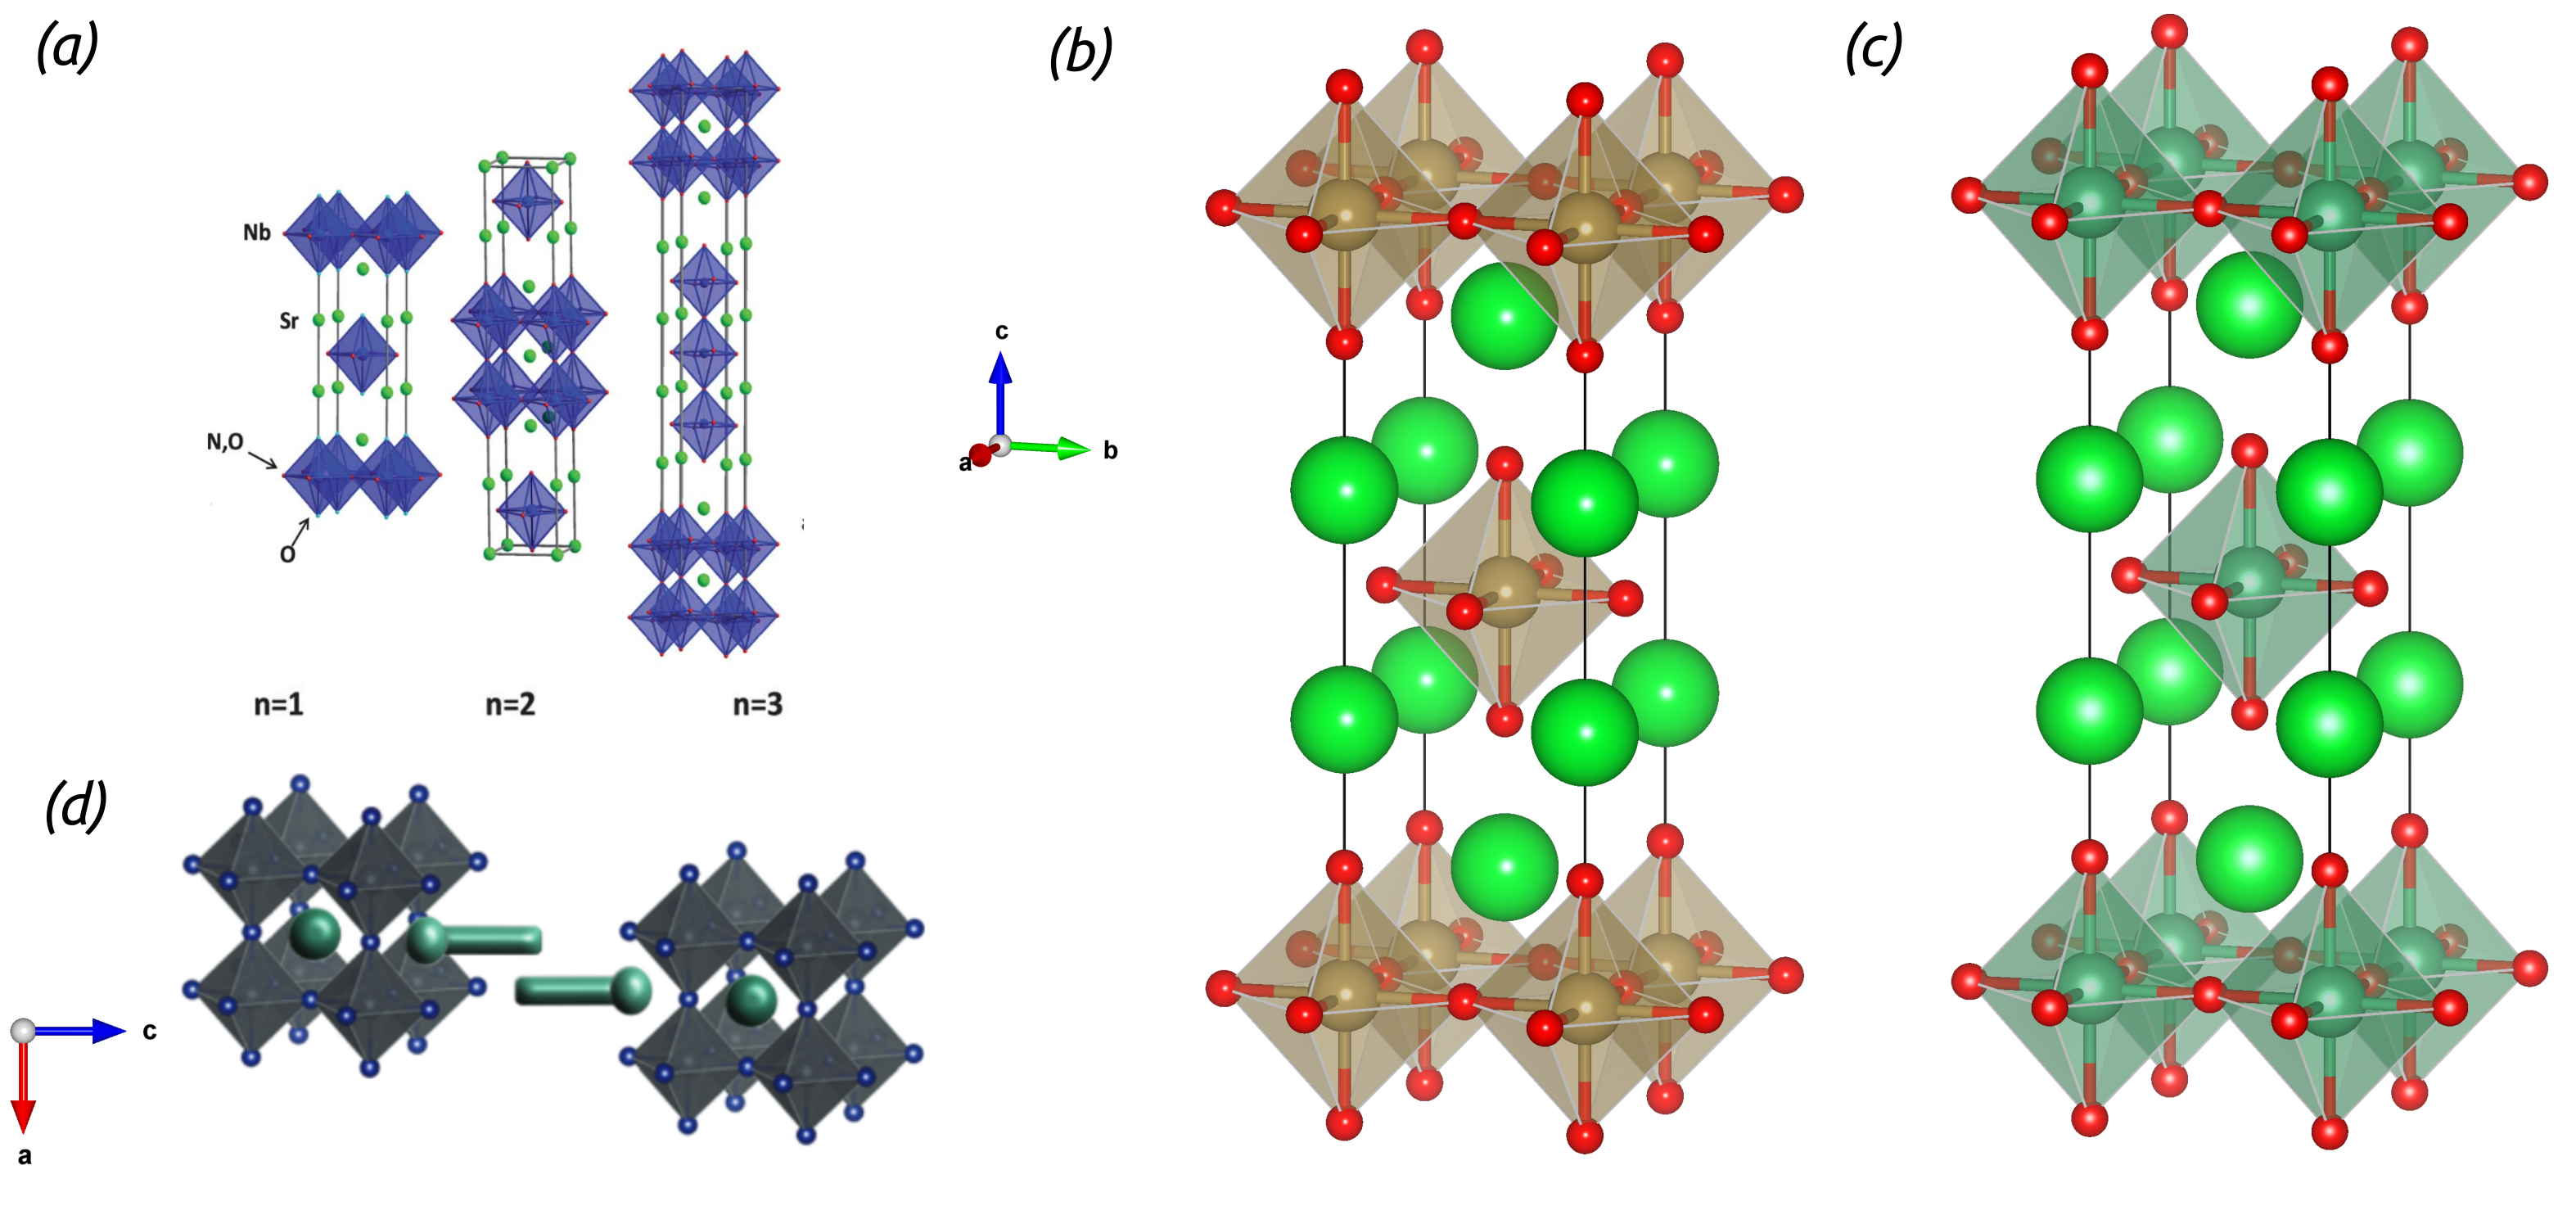
\includegraphics[width=13.0cm,keepaspectratio=true]{Figs/series-rp.png}
    \caption{Celda unitaria de la familia Ruddlesden-Popper para: (a) tres fases $(SrO) (SrNbO_{3})$ \cite{Fuertes2012ChemistryPerovskites}, la fase $n=1$ de (b) $Sr_{2}TaO_{4}$ y (c) $Sr_{2}NbO_{4}$. (d) Esquema estructural de \textsc{rp} \cite{milic2021Multi}.}
    \label{Fig. series-rp}
\end{figure}

En general, la investigación en sistemas por capas se ha extendido debido a posibles propiedades contenidas en los espacios entre capas dislocadas. Un ejemplo de ello es la tendencia por buscar nuevas fases superconductoras de sistemas laminares con metales de transición distintos del cobre\cite{Maeno1994SuperconductivityCopper}. En el caso de la familia Ruddlesden-Popper, el rompimiento del enlace debido a la dislocación de las capas (ver figura \ref{Fig. series-rp}d) permite aprovechar el espacio generado para enlazar elementos o moléculas, como lo evidencia Milić y su trabajo con materiales de perovskita de haluro por capas conectadas por restos orgánicos \cite{milic2021Multi}.  

\section{Oxinitruros}

Los oxinitruros tipo perovskitas son una clase emergente de material con propiedades ópticas, eléctricas, foto-catalíticas\cite{Pan2015Innentitelbild:10/2015}, dieléctricas y magnetorresistivas que pueden ser sensibles al orden óxido-nitruro. Se caracterizan por la disposición de los aniones de oxígeno y nitrógeno en las esquinas de los octaedros de la perovskita, lo que genera diferentes ordenamientos de oxígeno-nitrógeno en el octaedro, nombrados \emph{fac}, \emph{mer}, \emph{trans} y \emph{cis} (figura \ref{Fig. cis_fac_mec_trans}). El oxigeno y el nitrógeno tienen similitudes en electronegatividad, polarizabilidad, radio iónico y numero de coordinación, permitiendo la formación de fases similares cuando son combinados en una misma estructura\cite{Tobias2004,Yang2011}.

\begin{figure}[H]
    \centering
    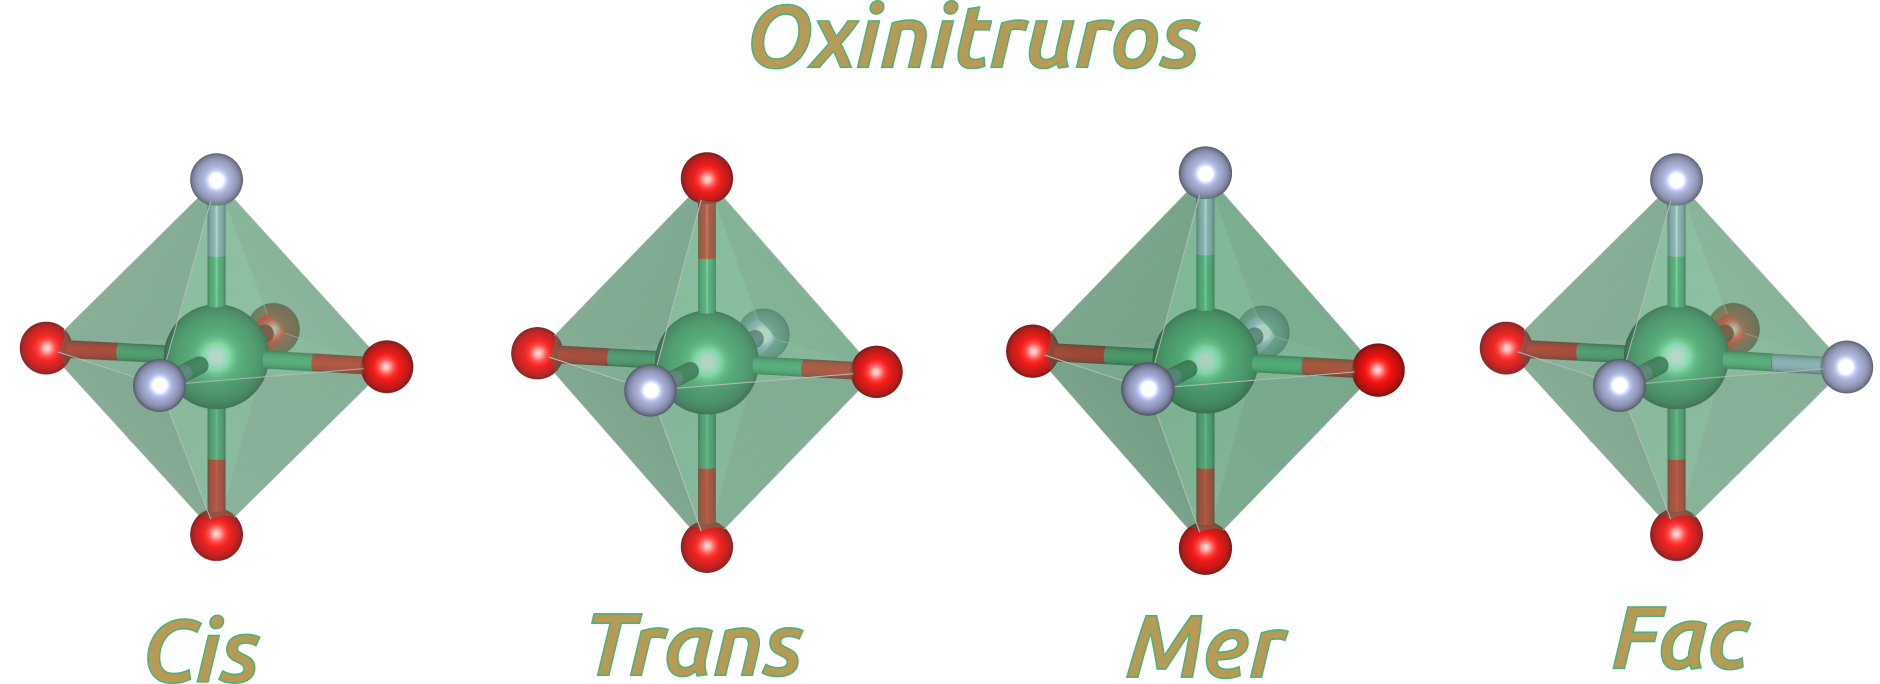
\includegraphics[width=8.0cm,keepaspectratio=true]{Figs/cis_trans_mer_fac.png}
    \caption{Combinación del oxígeno y el nitrógeno en el octaedro de la perovskita. Por notación, los aniones de oxigeno y nitrógeno son denotados en colores rojo y gris respectivamente.}
    \label{Fig. cis_fac_mec_trans}
\end{figure}

Su estabilidad a temperatura ambiente es mayor comparada con los nitruros puros, pero con brechas en la banda electrónica más pequeñas comparadas con los óxidos. Esto conduce al mejoramiento de propiedades ópticas y electrónicas que puedan existir en el material, tales como el dopado de nitrógeno ($N$) en el material $TiO_{2}$. El enlace covalente de $\text{metal}-N$ junto con el enlace $\text{metal}-O$ conlleva a una reducción de la brechas en la banda electrónica, permitiendo el ajuste de la absorción de luz desde la región ultravioleta a la región visible\cite{Gou2020Photocatalysis} para la fotocatálisis\cite{Ebbinghaus2004,Yang2011}.

La búsqueda de fotocatalizadores de luz visible para la división general del agua en hidrógeno y oxígeno es una tarea desafiante para resolver la crisis energética y la contaminación ambiental \cite{Cen2019OptimizedSplitting}. Por lo tanto, es muy deseable explorar oxinitruros de perovskita ferroeléctricos para fotocatálisis de alto rendimiento. A pesar de que estos sistema son la tecnología más nueva y han atraído nuevas investigaciones importantes sobre la generación de hidrógeno, hasta ahora, no se han realizado muchas investigaciones sobre materiales ferroeléctricos para su uso en sistemas de división de agua \cite{Gou2020Photocatalysis}, diseñando nuevas fases que se basan en sustituir el oxigeno por un anión similar en polarizabilidad y electronegatividad como el nitrógeno\cite{Rossell2012Auth}. La gran mayoría de oxifluoruros y oxinitruros exhiben ordenamientos aniónicos \emph{cis} y \emph{fac}, aunque estudios recientes han demostrado que puede inducir el orden de aniones \emph{trans}\cite{Harada2019}.



%\section{Motivación}

%A continuación se presentan dos interesantes propiedades del material perovskita tipo Ruddlesden-Popper: ferroelectricidad y actividad catalítica mediante luz para división de agua.

\section{Ferroelectricidad}

El concepto básico de ferroelectricidad fue introducido por Valasek en el sistema \textit{sal de Rochelle} en 1920 \cite{Valasek1921Piezo-electricSalt}: si se aplica un campo eléctrico externo a un material ferroeléctrico, los dipolos en la estructura cristalina son inducidos a producir una polarización espontánea y alineación con el campo externo, incluso cuando el campo eléctrico está apagado el material tiene polarización remanente que es su polarización espontánea. A esto se le llama fenómeno ferroeléctrico \cite{Kim2018FerroelectricSplitting}. En términos generales, el mecanismo de los ferroeléctricos puede ser categorizado en dos tipos: (1) de orden-desorden, para el cual la reorientación de iones de un estado desordenado a un estado ordenado conduce a la ferroelectricidad  y (2) de desplazamiento, para lo cual la ferroelectricidad surge del desplazamiento relativo de iones \cite{Kim2018FerroelectricSplitting,Shi2016SymmetryFerroelectrics}. 

En los sistemas cristalinos, hay $31$ grupos de punto que describen las simetrías de las estructuras cristalinas. estos grupos contienen transformaciones u operaciones de simetría como traslación, inversión, reflexión y rotación \cite{Glazer2013SpaceScientists}. De los $31$ grupos de punto solo $10$ son grupos polares, formalmente definidos como grupos con estructura no centro-simétrica. Esta definición es indispensable para hablar de sistemas ferroeléctricos, la estructura cristalina puede obtener una pequeña distorsión que rompe la simetría implicando un desplazamiento polar en los átomos de la celda unitaria. Los materiales ferroeléctricos son inseparables del rompimiento de simetría exhibiendo un fenómeno de transición de fase. Este rompimiento de la simetría es capturada por el parámetro de orden conocido como polarización espontánea que puede ser presentada en una fase con grupo de punto polar \cite{Rabe2007ModernFerro}. La transición de fase se lleva desde una fase paraeléctrica de alta temperatura y alta simetría a una fase ferroeléctrica de baja temperatura y baja simetría. En la fase paraeléctrica, existe una relación lineal entre la polarización (P) y el campo eléctrico (E), mientras que la curva no lineal que emerge en la fase ferroeléctrica se conoce como  curva de histéresis ferroeléctrica \cite{Shi2016SymmetryFerroelectrics} (figura \ref{Fig. p-e}). 

\begin{figure}[H]
    \centering
    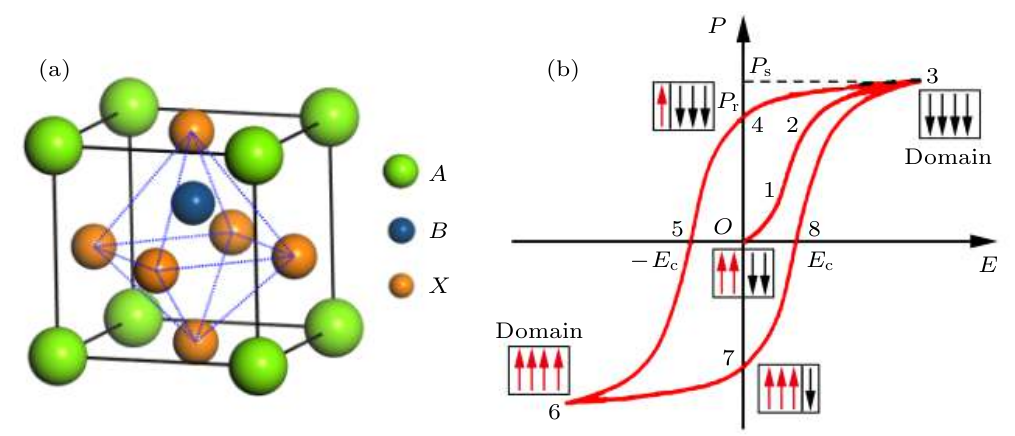
\includegraphics[width=0.9\textwidth]{Figs/polarization.png}
    \caption{(a)Estructura $ABX_{3}$ tipo perovskita. (b) Curva de histéresis \textsc{p-e} \cite{Cui2020ResearchSemiconductors}.}
    \label{Fig. p-e}
\end{figure}

Los materiales ferroeléctricos tienen propiedades útiles con un amplio rango de aplicabilidad. Algunos ejemplos son: Películas delgadas de $SrBi_{2}Ta_{2}O_{9}$ aplicada a memorias de acceso aleatorio ferroeléctricas (\textsc{fram}) \cite{Sreenivas1994film}. El material $LiNbO_{3}$ ferroeléctrico que exhibe fuertes efectos electro-ópticos aplicables en fotónica \cite{Whatmore2021celebrration}. Los oxinitruros de perovskita son aplicables como materiales ferroeléctricos \cite{Bouri2018} debido a la disposición e interacción entre el orden de aniones promoviendo ferroelectricidad \cite{Gou2020Photocatalysis,Yang_2015}, experimentalmente confirmado en la superficie de los materiales $SrTaO_{2}N$ y $Sr_{2}TaO_{3}N$\cite{Suemoto2018IntergrowthSr2TaO3N}. 

\section{Fotocatálisis}

La conversión directa de la luz solar en combustibles químicos mediante reacciones electroquímicas representa una alternativa limpia, sostenible y potencialmente barata a los combustibles fósiles, además de ser una tarea muy desafiante para resolver la crisis energética y la contaminación ambiental \cite{Cen2019OptimizedSplitting}. La reacción más simple de este tipo es la reacción de división de agua en la que el agua se divide en hidrógeno y oxígeno \cite{Castelli_2013}. Durante la fotocatálisis, el fotón absorbido excita un electrón a la banda de conducción, dejando un hueco en la banda de valencia. Los electrones y huecos foto-generados migrarán a la superficie para contribuir a la reducción y oxidación de las especies absorbidas, lo que finalmente resulta en la producción de $H_{2}$ y $O_{2}$ \cite{Bouri2018}.

Cualquier material empleado como fotocatalizador para división de agua debe cumplir con un conjunto de criterios: estabilidad química y estructural, una banda prohibida en el rango visible con un intervalo de banda óptimo ($\sim2eV$) \cite{Cen2019OptimizedSplitting}, bordes de banda bien posicionados con respecto a los niveles red-ox del agua, y alta movilidad de electrones y huecos. Además, se requieren bajos costos y no toxicidad \cite{Castelli_2013}. Los oxinitruros son prometedores fotocatalizadores \cite{Suemoto2018IntergrowthSr2TaO3N,kato2001,wang2015} debido a que contienen aniones con electronegatividad más débil en relación con el oxigeno ($O$), exhibiendo brechas de banda electrónica más pequeños que los óxidos de perovskita, lo que ajusta la absorción óptica desde el ultravioleta al rango visible del espectro solar \cite{Fuertes2015}. Entre los oxinitruros, la brecha de la banda electrónica reducida debido a la sensibilidad del orden oxinitrado \cite{Tobias2004,Yang2011} y la ferroelectricidad benefician la separación de pares de electrones-huecos foto-excitados, permitiendo que estructuras \textsc{rp} como $A_{2}BO_{3}N$ ($A=Cs,Ca,Sr,Ba$ y $ B=Ta,Nb)$ \cite{Cen2019OptimizedSplitting,Pan2018} muestren un rendimiento fotocatalítico prometedor en el espectro visible \cite{Gou2020Photocatalysis,siritanaratkul2011,ZHANG2019}.


\section{Teoría Funcional de la Densidad (DFT)}

La teoría funcional de la densidad es la base para los cálculos de optimización de la estructura, cálculos auto-consistentes de la estructura electrónica y estructura fonónica. Además, se tendrá en cuenta un término adicional llamado parámetro de Hubbard (\textsc{u}) para sistemas altamente correlacionados, debido a la correlación de los electrones en los metales de transición niobio ($Nb$) y tántalo ($Ta$) \cite{Tolba2018}.

La idea fundamental de la teoría funcional de la densidad consiste en que cualquier propiedad de un sistema de muchas partículas interactuantes puede ser visto como una funcional de la densidad del estado base $n_{0}(\Vec{r})$, es una teoría de un sistema de muchos cuerpos correlacionados y ha llegado a ser la herramienta principal para cálculos de estructura electrónica y otros sistemas finitos \cite{martin_2004}. La idea original parte del método de Thomas-Fermi\cite{Fermi1927StatisticalAtoms,Thomas1927TheFields}, la energía cinética de un sistema de electrones es aproximada como una funcional explicita de la densidad, idealizada como electrones no interactuantes en un gas homogéneo con densidad igual a la densidad local en cualquier punto dado. Tanto Thomas como Fermi no tuvieron en cuenta el intercambio y la correlación entre electrones, sin embargo, esto fue agregado por Dirac\cite{Dirac1930NoteAtom} en 1930, quien formuló la aproximación local para el intercambio de electrones.

\begin{equation}
    E_{TF}[n]=\int n(\vec{r})^{5/3}\mathrm{d}^{3}r+\int V_{ext}(\vec{r})n(\vec{r})\mathrm{d}^{3}r+ \int n(\vec{r})^{4/3}\mathrm{d}^{3}r+\frac{1}{2}\int  \frac{n(\vec{r})n(\vec{r'})}{|\vec{r}-\vec{r'}|}\mathrm{d}^{3}r
\end{equation}

El primer término es la aproximación local de la energía cinética, el tercer termino es el intercambio local y el ultimo termino es la energía electrostática de Hartree. La densidad y energía del estado base puede ser encontrado minimizando la funcional $E[n]$ para todos los posibles $n(\vec{r})$ sujeto a la restricción sobre el numero total de electrones.

\begin{equation}
    N=\int n(\vec{r})\mathrm{d}^{3}r
\end{equation}

Esta es una primera aproximación de la teoría funcional de la densidad, pero Hohenberg y Kohn le dan el enfoque para formular esta teoría como un teoría exacta de sistemas de muchos cuerpos. La formulación aplica para cualquier sistema de partículas interactuantes en un potencial externo $V_{ext}(\vec{r})$, incluyendo cualquier problema de electrones y núcleos fijos, donde el hamiltoniano puede ser escrito como:

\begin{equation}
    \hat{H}=-\frac{\hslash^{2}}{2m_{e}}\sum_{i}\nabla_{i}^{2}+\sum_{i}V_{ext}(\vec{r}_{i})+\frac{1}{2}\sum_{i\neq j}\frac{e^{2}}{|\vec{r}_{i}-\vec{r}_{j}|}
    \label{Eq. Hamiltonian_HK}
\end{equation}

\subsection{Teoremas de Hohenberg-Kohn}

La teoría funcional de la densidad esta basada en dos teoremas primeramente demostrados por Hohenberg y Kohn\cite{P.Hohemberg1964InhomogeneousGas}:

\begin{itemize}
    \item \textbf{Teorema 1:} Para cualquier sistema de partículas interactuantes en un potencial externo $V_{\text{ext}}(\vec{r})$, este potencial es determinado únicamente por la densidad de partículas del estado base $n_{0}(\vec{r})$.
    \item \textbf{Teorema 2:}  Una funcional universal para la energía $E[n]$ en términos de la densidad $n(\vec{r})$ puede ser definida, valida para cualquier potencial externo $V_{\text{ext}}(\vec{r})$. Para cualquier potencial particular $V_{\text{ext}}(\vec{r})$, el valor de energía exacta del estado base del sistema es un mínimo global de esta funcional, y  la densidad $n(\vec{r})$ que minimiza el funcional es la densidad exacta del estado base $n_{0}(\vec{r})$.
\end{itemize}

%\begin{itemize}
%   \item \textbf{Corolario 1:} Todas las propiedades del sistema están completamente determinadas dando solo la densidad del estado base $n_{0}(\vec{r})$.
%    \item \textbf{Corolario 2:} El funcional $E[n]$ es suficiente para determinar la energía y la densidad exacta del estado base.
%\end{itemize}

En principio, las funciones de onda $\Psi$ de cualquier estado están determinadas resolviendo la ecuación de Schrodinger con el hamiltoniano presente en la ecuación (\ref{Eq. Hamiltonian_HK}).  Entre todas las soluciones las cuales son consistentes con la densidad dada, la única función de onda $\Psi$ del estado base es la que tiene la menor energía. El teorema solo requiere que la densidad electrónica determine de forma única la posición y los tipos de núcleos, lo cual puede ser probado fácilmente desde la mecánica cuántica elemental. Pero aún existe el problema original de muchos electrones interactuantes moviéndose en el potencial debido a los núcleos. Como todas las propiedades del sistema, son determinadas de forma única si $n(\vec{r})$ es especificado, entonces cada propiedad puede ser vista como una funcional de $n(\vec{r})$, incluyendo la funcional de la energía total:

\begin{equation}
    \begin{split}
        E_{\textsc{hk}}[n]&=T[n]+E_{\text{int}}[n]+\int\mathrm{d}^{3}rV_{\text{ext}}(\vec{r})n(\vec{r})+E_{\textsc{ii}}\\
        &=F_{\textsc{hk}}[n]+\int\mathrm{d}^{3}rV_{\text{ext}}(\vec{r})n(\vec{r})+E_{\textsc{ii}}
    \end{split}
    \label{Eq. E_HK}
\end{equation}

Donde $E_{\textsc{ii}}$ es la energía de interacción del núcleo, el termino $F_{\textsc{hk}}[n]$ incluye  las energías internas, cinética y potencial del sistema de electrones. Entonces un funcional puede ser definido por cualquier densidad, y minimizando este funcional se puede encontrar la densidad y la energía exacta para un sistema interactuante de muchos cuerpos \cite{martin_2004}. Un interesante punto es que un sistema con una polarización neta con campo eléctrico $\vec{E}=0$ como lo es un ferroeléctrico, la polarización es determinada solo por la densidad\cite{Martin1997FunctionalSystems,Martin1997RecentSolids}, es decir el teorema original de Hohenberg-Kohn si aplica. Los teoremas están en términos de funcionales de la densidad desconocidos, y es demostrable que estos deben ser funcionales no locales, dependiendo simultáneamente sobre $n(\vec{r})$ con posiciones diferentes de $\vec{r}$. Si el funcional $F_{\textsc{hk}}[n]$ es conocido, se puede minimizar la energía total del sistema respecto a las variaciones en la densidad electrónica, y se podría encontrar la densidad y energía exacta del estado base. Este es el problema central en la aproximación Kohn-Sham para la teoría funcional de la densidad. 

%Puede uno fácilmente construir diferentes funciones de onda $\Psi$ que tienen la misma densidad $n(\vec{r})$?. Todas las funciones de onda tienen la misma densidad uniforme, pero solo la elección del estado de energía cinética mas bajo da el estado base de energía mas bajo para el caso no interactuante. Los electrones interactuantes también tienen la misma densidad uniforme aunque las funciones de onda son correlacionadas, por lo tanto bastante diferente de un solo determinante.

%Susceptibilidades estáticas son dadas correctamente por el funcional del estado base? Todas las susceptibilidades estáticas son segundas derivadas de las energías del estado base con respecto a los campos externos. Entonces ellos deben ser dados correctamente por la variación del funcional Hohenberg-Kohn del estado base como funciones de campos externos.\\

\subsection{Aproximación de Kohn-Sham}

La teoría funcional de la densidad es hoy el método mas usado ampliamente para cálculos de estructura electrónica debido a la aproximación propuesta por Kohn y Sham en 1965\cite{Kohn1965Self-consistentEffects} para reemplazar el problema original de muchos cuerpos por un problema auxiliar de partícula independiente. La formulación básica de la aproximación de Kohn-Sham y la idea detrás del ingrediente crucial es el funcional de energía de intercambio-correlación $E_{xc}[n]$. La densidad del estado base del sistema original interactuante es igual a cualquier sistema no interactuante. Esto lleva a ecuaciones de partículas independientes para el sistema no interactuante que puede ser resuelto exactamente con toda la dificultad de los términos de muchos cuerpos, pero estos términos son incorporados dentro del funcional de la densidad de intercambio-correlación. Para resolver las ecuaciones se debe encontrar la densidad y la energía del estado base del sistema original interactuante con la precisión limitada solo por las aproximaciones en el funcional de intercambio-correlación\cite{martin_2004}. La construcción de Kohn-Sham de un sistema auxiliar recae en dos proposiciones:

\begin{itemize}
    \item La densidad exacta del estado base puede ser representada por la densidad del estado base de un sistema auxiliar de partículas no interactuantes. 
    \item El hamiltoniano auxiliar es elegido para tener un usual operador cinético y un potencial local efectivo $V_{\text{eff}}^{\sigma}(\vec{r})$ que actúa sobre un electrón en el punto $\vec{r}$.
\end{itemize}

Para un sistema de electrones independientes que obedecen el hamiltoniano, el estado base tiene un electrón $N$ en cada uno de los orbitales $\Psi_{i}(\vec{r})$ con los autovalores $\epsilon_{i}$ mas bajos del hamiltoniano. La densidad del sistema auxiliar esta dada por la suma del cuadrado de los orbitales:

\begin{equation}
    n(\vec{r})=\sum_{i=1}^{N}|\Psi_{i}(\vec{r})|^{2}
    \label{Eq. density-elec}
\end{equation}

La energía cinética de partículas independientes $T_{s}$ esta dada por:

\begin{equation}
    \begin{split}
       T_{s}=&-\frac{1}{2}\sum_{i=1}\braket{\Psi_{i}|\nabla^{2}|\Psi_{i}}\\
       =&\frac{1}{2}\sum_{i=1}\int\mathrm{d^{3}}r|\Psi_{i}(\vec{r})|^{2}
    \end{split}
\end{equation}

La energía cinética de partícula independiente $T_{s}$ es dada explícitamente como un funcional de los orbitales, y la clásica energía de interacción de Coulomb de la densidad electrónica $n(\vec{r})$ que interactúa consigo mismo es:

\begin{equation}
    E_{\text{Hartree}}[n]=\frac{1}{2}\int\mathrm{d^{3}}r\mathrm{d^{3}}r'\frac{n(\vec{r})n(\vec{r'})}{|\vec{r}-\vec{r'}|}
\end{equation}

La aproximación de Kohn-Sham para el problema de muchos cuerpos interactuantes es para reescribir la expresión de Hohenberg-Kohn para el funcional de energía del estado base en la siguiente forma:

\begin{equation}
    E_{\textsc{ks}}=T_{s}[n]+\int\mathrm{d}rV_{\text{ext}}(\vec{r})n(\vec{r})+E_{\text{Hartree}}[n]+E_{\textsc{ii}}+E_{xc}[n] 
    \label{Eq. KS}
\end{equation}

Aquí $V_{\text{ext}}$ es el potencial externo debido a los núcleos y cualquier otro campo externo, y $E_{\textsc{ii}}$ es la interacción entre los núcleos. Todos los efectos de intercambio y correlación de muchos cuerpos son agrupados en un funcional de intercambio-correlación $E_{xc}$, que puede ser escrito en términos del funcional de Hohenberg-Kohn como:

\begin{equation}
    \begin{split}
        E_{xc}[n]=&F_{\text{hk}}[n]-(T_{s}[n]+E_{\text{Hartree}}[n])\\
        =&\braket{\hat{T}}-T_{s}[n]+\braket{\hat{V}_{\text{int}}}-E_{\text{Hartree}}[n]
    \end{split}
\end{equation}

La ultima ecuación muestra explícitamente que $E_{xc}$ es solo la diferencia de energía cinética y las energías de interacción interna del sistema interactuante de muchas partículas con las interacciones electrón-electrón reemplazado por la energía de Hartree. Si el funcional universal $E_{xc}$ fuese conocido, entonces la energía y densidad exacta del estado base del problema de muchos cuerpos del electrón podría ser encontrado resolviendo las ecuaciones de Kohn-Sham para partículas independientes. El potencial de Kohn-Sham esta definido como:

\begin{equation}
    V_{\textsc{ks}}=V_{\text{ext}}(\vec{r})+V_{\text{Hartree}}(\vec{r})+V_{xc}(\vec{r})
    \label{Eq. V_ks}
\end{equation}  

El potencial de intercambio-correlación $V_{xc}$ es el funcional derivado de $E_{xc}$, el cual puede ser escrito como:


\begin{equation}
    V_{xc}(\vec{r})=\epsilon_{xc}([n],\vec{r})+n(\vec{r})\frac{\delta\epsilon_{xc}([n],\vec{r})}{\delta n(\vec{r})}
    \label{Eq. V_xc}
\end{equation}

Donde $\epsilon_{xc}([n],\vec{r})$ es una energía por electrón en el punto $\vec{r}$ que solo depende de la densidad $n(\vec{r})$. El segundo termino denominado potencial de respuesta\cite{Gritsenko1994AnalysisPotentials}. En un aislante, esta derivada es discontinua en un bandgap donde la naturaleza de los estados cambia discontinuamente como función de $n$. Esto lleva a una derivada discontinua por lo cual el potencial para todos los electrones en un cristal cambia por una cantidad constante cuando un electrón es agregado\cite{Perdew1983PhysicalDiscontinuities,Sham1983Density-functionalGap}. Agregar un electrón puede variar el potencial para todos los otros electrones en un solido. El gran avance del enfoque de Kohn-Sham sobre la aproximación del Thomas-Fermi es la incorporación de orbitales para definir la energía cinética. En términos de orbitales, es fácil ver que la energía cinética $T_{s}$ para partículas independientes cambia discontinuamente en irse desde una banda ocupada a una banda vacía, ya que $\Psi_{i}(\vec{r})$ son diferentes para cada banda \cite{martin_2004}.

La aproximación Kohn-Sham pone mas énfasis sobre el estado base que los teoremas de Hohenberg-Kohn. Las únicas propiedades  garantizadas a ser correctas por construcción en la teoría exacta de Kohn-Sham son la densidad y la energía. La construcción de un sistema auxiliar lleva a tratables ecuaciones de partícula independiente que guarda la esperanza de resolver problemas de muchos cuerpos interactuantes\cite{martin_2004}.

%Es la densidad de espín correcta en la teoría de Kohn-Sham? Si, Un potencial efectivo dependiente del espín es introducido específicamente para dar la correcta densidad y densidad de espín.

%Son la carga estática y las susceptibilidades de espín dadas correctamente por el funcional del estado base? Si, todas las susceptibilidades estáticas son segundas derivadas de las energías del estado base con respecto a campos externos. Entonces ellos deben ser dados correctamente por la variación del funcional Kohn-Sham del estado base como funciones de campos externos.

%Es la superficie de Fermi exacta de un metal dada correctamente por los autovalores en la teoría exacta de Kohn-Sham? No, aunque la densidad es reproducida, la superficie de Fermi no podría ser correcta debido a los requerimientos de un potencial local.[357]

%DEbe un aislante de Mott -un aislante debido a las correlaciones entre electrones- ser predicho correctamente por los autovalores en la teoria exacta de Kohn-Sham? No, Esto sigue desde los argumentos de arriba sobre un metal que la superficie de Fermi no es correcta en general.

%Son energia de excitacion dada correctamente por los autovalores de las ecuaciones de Kohn-Sham? No, los autovalores no son las verdaderas energias para agregar o substraer electrones, no para excitaciones neutrales.

%Es alguna energia de excitacion dada correctamente por los autovalores de las ecuaciones de Kohn-Sham? Si, el autovalor mas alto en un sistema finito debe ser correcto[354] desde que el estado domina el largo alcance de la densida, el cual es definido para ser correcto.

%Es exacto el calor especifico y la temperatura dada correctamente por el funcional exacto de Mermin de temperatura finita? Si, aunque el calor especifico envielve excitaciones desde el estado base, sin embargo los promedios termicos sobre estas escitaciones deben ser una unica funcional de la desidad y la temperatura. No obstante, es mas dificil derivar el funcional de intercambio-correlacion como funcion de la temperatura.

%Es posible determinar las energias de excitacion por algun medio usando la teoria de Kohn-Sham? Si, la pregunta esta en el espiritu de las pruebas existentes de Hohenberg-Kohn. Desde la densidad de Kohn-Sham es exacta por construccion, esto sigue desde los teoremas de Hohenberg-Kohn que todas las porpiedades estan determinadas desde que el hamiltoniano entero es determinado.\\

\subsection{Aproximación de la densidad local (LDA)}

El funcional de intercambio-correlación $E_{xc}[n]$ puede ser razonablemente aproximado como un funcional local o cercanamente local de la densidad. La energía de intercambio-correlación es simplemente una integral sobre todo el espacio con la densidad de energía de intercambio-correlación en cada punto asumido a ser el mismo en un gas homogéneo de electrones:

\begin{equation}
    \begin{split}
        E_{xc}^{\textsc{lsda}}[n]=&\int\mathrm{d}^{3}rn(\vec{r})\epsilon_{xc}^{\text{hom}}(n(\vec{r}))\\
        =&\int\mathrm{d}^{3}rn(\vec{r})[\epsilon_{x}^\text{hom}(n(\vec{r}))+\epsilon_{c}^\text{hom}(n(\vec{r}))]
    \end{split}
    \label{Eq. energy_lsda}
\end{equation}

La única información necesaria es la energía de intercambio-correlación del gas homogéneo como una función de la densidad; la energía de intercambio del gas homogéneo es dada por una forma analítica simple y la energía de correlación ha sido calculada con gran precisión por los métodos Monte Carlo\cite{Ceperley1980GroundMethod}.

\subsection{Aproximación de gradiente generalizado (GGA)}

El éxito de \textsc{lda} ha llevado al desarrollo de varias aproximaciones de gradiente generalizado con una gran mejora sobre \textsc{lda} para muchos casos. \textsc{gga}\cite{Perdew1996ComparisonFunctional} es una funcional dependiente de la magnitud del gradiente de la densidad $|\nabla n|$, así como del valor de $n$ en cada punto. Es conveniente definir el funcional como una forma generalizada de (\ref{Eq. energy_lsda}):

\begin{equation}
    \begin{split}
        E_{xc}^{\textsc{gga}}[n]=&\int\mathrm{d}^{3}rn(\vec{r})\epsilon_{xc}(n,|\nabla n|...)\\
        \equiv&\int\mathrm{d}^{3}rn(\vec{r})\epsilon_{x}^\text{hom}(n)F_{xc}(n,|\nabla n|,...)
    \end{split}
\end{equation}

Donde $F_{xc}$ es adimensional y $\epsilon_{x}^{\text{hom}}(n)$ es la energía de intercambio de un gas. Numerosas formas para $F_{xc}$ han sido propuestas, estas pueden ser ilustradas por tres formas ampliamente usadas, como Becke (\textsc{b88})\cite{Becke1988Density-functionalBehavior}, Perdew an Wang (\textsc{pw91})\cite{Perdew1992AccurateEnergy}, y Perdew, Burke, and Enzerhof (\textsc{pbe})\cite{Perdew1996GeneralizedSimple}. Todos los \textsc{gga} dejan una energía de intercambio mas baja que \textsc{lda}, hay regiones de densidad que varían mas rápidamente en átomos, el cual lleva a una mayor reducción de la energía de intercambio en átomos que en moléculas y solidos. Esto resulta en la reducción de la energía de enlace, corrigiendo el sobre-enlazamiento de \textsc{lda}, y mejorando los resultados respecto a los experimentos, siendo una de las mas importantes características de \textsc{gga} \cite{martin_2004}.% Incluso si una forma de \textsc{gga} de alguna manera da los resultados correctos para una cierta propiedad física mientras que para otras falla, no es garantía que la forma es superior  para otras propiedades físicas en la cual diferentes condiciones físicas prevalecen.

Los  problemas de intercambio y correlación son mas severos en materiales en los que los electrones tienden a ser localizados y fuertemente interactuantes, como los óxidos de metal de transición y elementos de tierras raras. Varios métodos han sido desarrollados para extender el enfoque funcional incorporando efectos que son esperados a ser importantes sobre la física base, estos son \textsc{sic}, \textsc{lda+u} y funcionales híbridos. \textsc{sic} es un método que usa funcionales aproximados y agrega una 'corrección auto-consistente' para intentar corregir la auto-interacción poco física en muchos funcionales de intercambio-correlación $E_{xc}$. Por otro lado, \textsc{lda+u} es usado en métodos que involucran el tipo de cálculos \textsc{lda} o \textsc{gga} acoplados con una interacción adicional a la dependencia del orbital \cite{Anisimov1997First-principlesMethod}. Funcionales híbridos son una combinación de Hartree-Fock dependiente de orbital y un funcional de densidad explicita. la definición de la energía intercambio-correlación dentro de los funcionales híbridos es:

\begin{equation}
    E_{xc}=E_{xc}^{\textsc{lda}}+a_{0}\left(E_{x}^{\textsc{hf}}-E_{x}^{\textsc{dfa}}\right)+a_{x}E_{x}^{\text{Becke}}+a_{c}E_{c}
\end{equation}

Con los coeficientes empíricamente ajustados a datos atómicos y moleculares.

%Para cualquier problema de un electrón, Hartree-Fock provee la solución exacta para la energía total y el autovalor mas bajo de la ecuación de Hartree-Fock (3.45) es la energia exacta para remover un electron. Esto es porque no hay correlacion y el potencial de intercambio (3.48) exactamente cancela la auto interaccion en el potencial de Hartree. Sin embargo, los autovalores del estado excitado de  (3.45) denotan la energia para agregar un segundo electron asuminedo que no hay correlacion y no hay cambios en el orbital ocupado. A veces hay errores muy grandes en las energias de adicion, for ejemplo para el atomo $H$ tratado por Hartree-Fock, no hay estados de enlace para electrones agregados, mientras que de hecho un segundo electron es enlazado por una pequeña energia.

%En la otra mano, los porblemas de una particula son fuertes pruebas para funcionales aproximados como \textsc{lda} y \textsc{gga}. Los funcionales son diseñados para tratar con muchos electrones (un gas homogeneo) y su aplicacion al problema de un electron introduce terminos poco fisico: (1) la auto iteraccion poco fisica en el termino de Hartree no es cancelada exactamente por el funcional de intercambio aproximado, y (2) es falso introducir un funcional de correlacion  dentro de un problema de una particula.

\section{Correlación electrónica: DFT+U}

En \textsc{dft}, las energías de interacción electrónica se describen simplemente como la suma de la repulsión columbiana  entre las densidades electrónicas (término de Hartree) y un término aditivo de todas las correlaciones e interacciones de espín \textit{xc}. Este término aditivo (\textit{xc}) se basa en aproximaciones que  recuperan la descripción exacta de la energía del sistema, es una funcional de la densidad de carga electrónica del sistema, y la precisión de un cálculo de \textsc{dft} depende en gran medida de esta funcional \textit{xc}. En general, es difícil modelar la densidad funcional de carga electrónica \textit{xc} y, por lo tanto, puede representar inadecuadamente las características de muchos cuerpos del estado fundamental de N-electrones. Por esta razón, los sistemas correlacionados están mal descritos por los cálculos de \textsc{dft}, la descripción incorrecta de la estructura electrónica induce el llamado "problema de bandagap", que a su vez impone dificultades en la utilización de \textsc{dft} para predecir interacciones intermoleculares precisas, energías de formación y estados de transición\cite{Tolba2018}. Basado en el modelo Hubbard, se construye el esquema \textsc{dft+u}, que es uno de los enfoques correctivos empleados para corregir el problema de "bandgap electrónico". Esta corrección \textsc{u} se puede agregar a los funcionales de densidad  \textsc{lda+u} y \textsc{gga+u}. El papel básico de la corrección \textsc{u} es tratar la fuerte interacción de Coulomb de sitio de los electrones localizados con un término adicional. El Hamiltoniano de Hubbard describe los estados electrónicos fuertemente correlacionados ($ d $ y $ f $ orbitales). En la implementación de \textsc{dft+u}, la fuerza de las interacciones en el sitio se describe mediante un par de parámetros: el término de Coulomb en el sitio \textsc{u} (Liechtenstein\cite{Lichtenstein1995StrongOrdering}) y el intercambio de sitio \textsc{j}. En general, $ U_{\text{eff}}=U-J$ (Dudarev\cite{Dudarev1998Electron-energy-lossStudy}) es usado debido a que el parámetro \textsc{j} es crucial para describir la estructura electrónica de materiales con acoplamiento espín orbita fuerte. En comparación con los enfoques alternativos, como los funcionales híbridos y los métodos post-Hartree-Fock, la corrección \textsc{dft+u} puede mejorar aún más la descripción de la estructura electrónica, incluidas las propiedades magnéticas y estructurales de los sistemas correlacionados, la energía de transferencia de electrones y las reacciones químicas, además de ser computacionalmente menos costoso. Para cada átomo, se encuentra que el valor \textsc{u} depende de los parámetros específicos del material, incluida su posición en la red y las propiedades estructurales. El valor de \textsc{u} depende del material, además de ser variable entre el nivel de teoría utilizado. En general, cuanto más localizado es el sistema, más sensible es al valor de \textsc{u}\cite{Tolba2018}.

%Computacionalmente, la primera linea activa la corrección de \textsc{U} para la aproximación de correlación-intercambio \textsc{lda}. Las segunda linea especifica el tipo de corrección a realizan, ya sea una corrección de Liechtenstein (1), o Dudarev (2). La tercera linea se refiere al elemento a ser corregido (2 para orbitales $d$), el valor $-1$ indica que no se debe realizar la corrección. La cuarta y quinta linea dependen de la linea dos y del elemento a ser corregido\cite{urlwikivasp}, los valores de \textsc{u} se calculan para átomos individuales.

Experimentalmente, se observa que los electrones de valencia se localizan en sus orbitales debido a fuertes correlaciones, mientras que en \textsc{dft}, los funcionales \textit{xc} tienden a deslocalizarlos excesivamente,  por lo tanto subestima el bandgap  y puede llegar a una predicción falsa del comportamiento de sistemas correlacionados. \textsc{u} puede inducir la localización electrónica debido a la cuenta explícita de las interacciones electrónicas en el sitio\cite{Tolba2018}. La energía total del sistema ($E_{\textsc{lda+u}}$) es la suma de la energía funcional estándar \textsc{lda} para todos los estados y la energía del funcional Hubbard que describe los estados correlacionados. Debido al término aditivo de Hubbard, habrá un doble error de conteo para los estados correlacionados; por lo tanto, se debe deducir un término de "doble conteo" ($E_{dc}$) de la energía total de \textsc{lda} que describe las interacciones electrónicas:

$$E_{\textsc{lda}}+U[\rho(r)]=E_{\textsc{lda}}[\rho(r)]+ E_{\text{Hub}}[{n_{mm}^{I\sigma}}]-E_{dc}[n^{I\sigma}]$$




%Es la polarización macroscópica en un cristal dado correctamente por la teoría de Kohn-Sham en términos de la densidad $n(\vec{r})$ en el 'bulk' del cristal? No, hace tiempo se sabe que la polarizacion no podira ser derivada simplemente desde la densidad. Recientes desarollos deerivan la polarizaccion de las fases de las funciones de onda, no dadas correctamente por los orbitales de Kohn-Sham.


%La interacción adicional es usualmente considerada solo para orbitales atómicos altamente localizados sobre el mismo sitio, es decir la misma forma como la interacción de \textsc{'u'} en modelos de Hubbard[392,393]. El efecto del termino agregado es de desplazar los orbitales localizados respecto a los otros orbitales, los cuales intentan corregir errores conocidos por ser grandes en los cálculos usuales de \textsc{lda} o \textsc{gga}.\\

%Los cálculos de bandas realizados previamente en \textsc{vasp}\cite{urlvasp} para las estructuras $Sr_{2}AO_{3}N$(A=Nb, Ta) tienen inconsistencias respecto a los resultados tanto computacionales como experimentales que mencionan un estrechamiento del bandgap en el nivel de Fermi ocasionado por el levantamiento de la banda de valencia del nitrógeno\cite{Diot1999CrystalN,Bouri2018BulkSr2TaO3N} , lo que indica que el sistema debe ser aislante. Según nuestros resultados el sistema es metal, es decir no existe brecha entre bandas en el punto $\Gamma$ de la zona de Brillouin, lo cual es incorrecto.\\


%%%%%%%%%%%%%%%%%%%%%%%%%%%%%%%%%%%%%%%%%%%%%%%%%%%%%%%%%%%%%%%%%%%%%%%%%%%%%%%%%%%%%%%%%%%%%%%%%%%%%%%%%%%%%%%%%%%%%%%%%%%%%%%%%%%%%%%%%%%%%%%%%%%%%%%%%%%%
%%%%%%%%%%%%%%%%%%%%%%%%%%%%%%%%%%%%%%%%%%%%%%%%%%%%%%%%%%%%%%%%%%%%%%%%%%%%%%%%%%%%%%%%%%%%%%%%%%%%%%%%%%%%%%%%%%%%%%%%%%%%%%%%%%%%%%%%%%%%%%%%%%%%%%%%%%%%


\section{Aproximación armónica}

Los fonones son vibraciones de la red cristalina, juegan un rol esencial en el comportamiento dinámico de la estructura y sus propiedades térmicas \cite{Togo2015phonopy}. Si consideramos una red cristalina con dos tipos de átomos en su celda unitaria, las frecuencias permitidas de la onda propagada debido al desplazamiento de los átomos se pueden clasificar en dos tipos: un fonón que cae a frecuencia cero en el punto $\Gamma$ de la zona de Brillouin llamado fonón acústico, y otro fonón con frecuencia diferente de cero en el punto $\Gamma$ llamado fonón óptico \cite{Hamid2018Solids}. En este sentido, los átomos se mueven alrededor de su posición de equilibrio $\vec{R}_{ni}$ con desplazamientos $\vec{S}_{ni}$, donde $ni$ corren sobre cada celda unitaria y sobre cada átomo en la celda unitaria, respectivamente. El cambio en la energía potencial $\Delta U$ es el enfoque en la aproximación armónica, el cual consiste en definir $\Delta U$ en función de una expansión en series de Taylor de los desplazamientos iónicos $\vec{S}_{ni}$ manteniendo los términos de segundo orden \cite{kaxirasjoannopoulos2019}:

\begin{equation}
    \Delta U =\frac{1}{2}\sum_{ni\alpha,mj\beta}S_{ni\alpha}\frac{\delta^{2}E^{\text{tot}}}{\delta R_{ni\alpha}\delta R_{mj\beta}}S_{mj\beta}
\end{equation}

Siendo la matriz constantes de fuerza la segunda derivada de la energía total respecto a posiciones atómicas de equilibrio. El tamaño de esta matriz es $ni\alpha$, que corren sobre cada celda unitaria, sobre cada átomo en la celda unitaria y sobre cada coordenada cartesiana, respectivamente. Ahora se definen los vectores de desplazamiento iónico $\vec{u}_{ni\alpha}$ para construir la ecuación de valores y vectores propios para fonones:

\begin{equation}
    \sum_{m,j,\beta}\vec{D}_{ni\alpha,mj\beta}\vec{u}_{mj\beta}=\omega^{2}\vec{u}_{ni\alpha}
    \label{valores-propios_phon}
\end{equation}

La frecuencia imaginaria, o valores propios negativos pueden aparecer en la solución de la ecuación \ref{valores-propios_phon}, lo que indica inestabilidad dinámica del sistema, ó llamados modos suaves, normalmente se obtienen con frecuencias por debajo de $100-200cm^{-1}$. $\vec{D}_{ni\alpha,mj\beta}$ representa la matriz dinámica:

\begin{equation}
    \sum_{m,j,\beta}\vec{D}=\sum_{m,j,\beta}\frac{1}{\sqrt{M_{i}M_{j}}}\vec{F}_{ni\alpha,mj\beta}
\end{equation}

La solución de esta ecuación son los valores propios representados por la frecuencia al cuadrado, y los vectores propio que describen los correspondientes desplazamientos iónicos \cite{kaxirasjoannopoulos2019}. La ecuación \ref{valores-propios_phon} puede ser descrita en función del vector de onda $\vec{k}$ aplicando el teorema de Bloch y condiciones de periodicidad:

\begin{equation}
    \vec{D}(\vec{k})\cdot\vec{u}_{\vec{k}}^{(l)}=\left(\omega_{\vec{k}}^{(l)}\right)^{2}\vec{u}_{\vec{k}}^{(l)}
    \label{valores-propios_phon-k}
\end{equation}

Donde $(l)$ representa el fonón en cada frecuencia. Esto para reducir la ecuación \ref{valores-propios_phon} y la matriz dinámica $d\times n_{a}$, donde $d$ es el número de celdas unitarias y $n_{a}$ el numero de átomos en cada celda unitaria. Para estructuras con átomos por celda unitaria $n_{a}$, hay $3\times n_{a}$ modos por cada valor de $\vec{k}$, por ejemplo para un sistema con dos átomos por celda unitaria hay tres fonones acústicos y tres fonones ópticos \cite{kaxirasjoannopoulos2019}. % Conjunto estabilizante para sistemas LTI
% ------------------------------------------------------------------------
% ------------------------------------------------------------------------
% ------------------------------------------------------------------------
%                                Capítulo 3
% ------------------------------------------------------------------------
% ------------------------------------------------------------------------
% ------------------------------------------------------------------------
\chapter{BÚSQUEDA DE LOS OXINITRUROS RP MÁS ESTABLES}\label{Cap. 2}

Este capítulo presenta un análisis estructural de los oxinitruros \textsc{rp} $Sr_{2}(Ta,Nb)O_{4-x}N_{x}$ y la búsqueda de los ordenamientos aniónicos más estables. Inicia con una breve descripción de óxidos de perovskitas \textsc{rp}, luego describe la substitución aniónica parcial $x=0.5$ de $O^{2-}$ por $N^{3-}$, y la substitución parcial $x=1$ de $O^{2-}$ por $N^{3-}$. Las substituciones aniónicas se realizan con el programa \textsc{sod}\cite{Grau-Crespo2007}, el cual es un paquete de herramientas para modelado computacional de sistemas periódicos con desorden substitucional de sitio. Un sistema desordenado es modelado como una copia de la celda, en donde combinaciones diferentes de desorden son puestas en los sitios cristalográficos. La celda diferente a la celda original es llamada \textit{'configuración'}. El proceso de identificar la simetría de cada configuración se realiza con las operaciones de simetría del grupo cristalográfico al que corresponde. Posteriormente, se identifican las configuraciones simétricamente equivalentes, y solo las configuraciones con simetría única son tomadas en cuenta. Una vez se identifican las configuraciones únicas, el código \textsc{sod} muestra las configuraciones únicas, y su degenerancia, es decir las configuraciones equivalentes \cite{Grau-Crespo2007}.

%sustituye los átomos y calcula las ocupaciones de sitio dando un numero de configuraciones resultantes. Mediante la simetría cristalina de la red, el programa reduce el número de configuraciones, identifica las configuraciones inequivalentes con el grupo de simetría espacial, es decir, calcula la degenerancia de las configuraciones.

\begin{figure}[H]
    \centering
    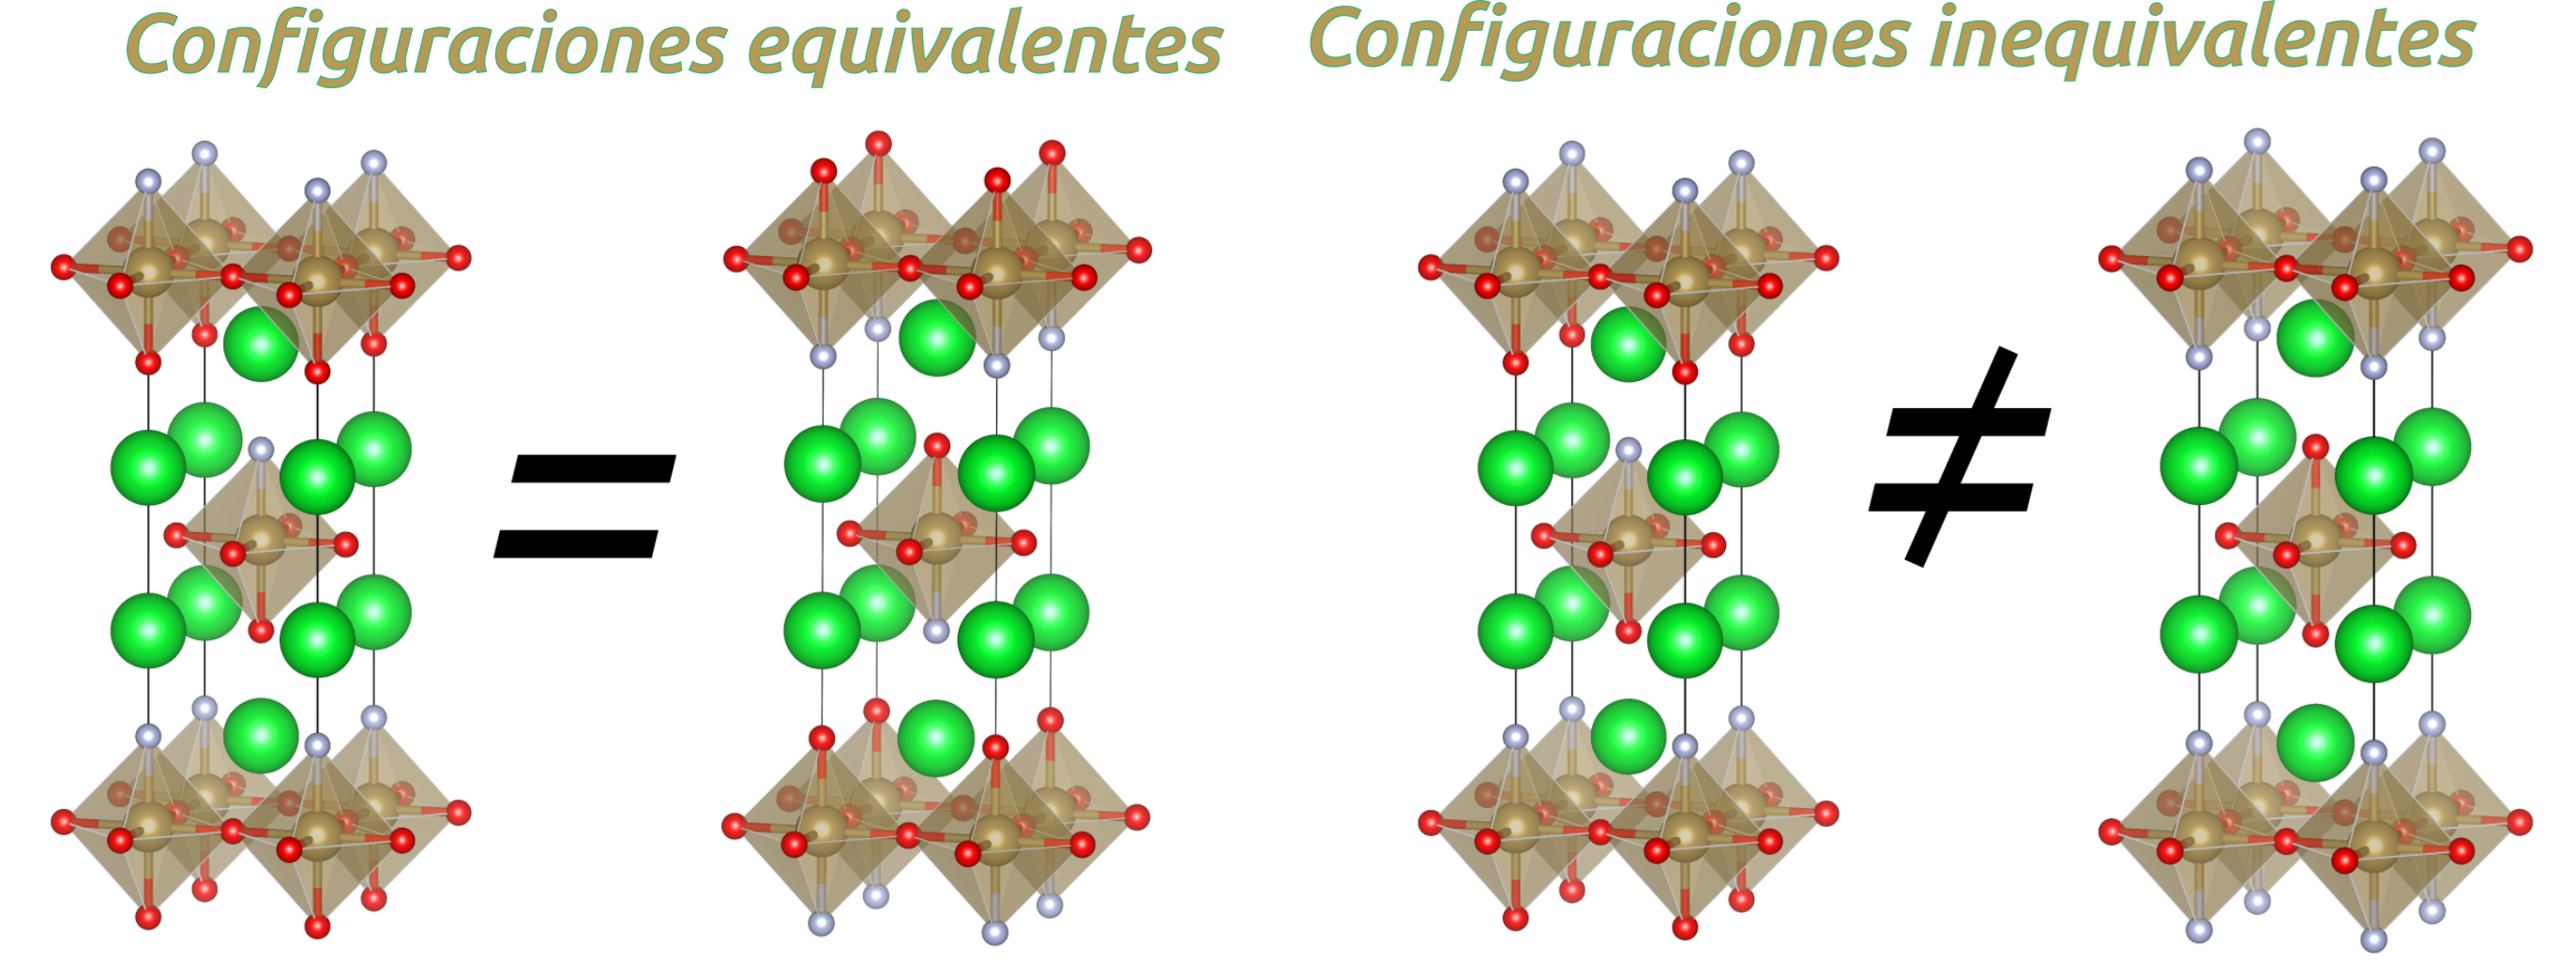
\includegraphics[width=0.9\textwidth]{Figs/config.png}
    \caption{Comparación de configuraciones equivalentes y configuraciones inequivalentes.}
    \label{Fig. config}
\end{figure}

El criterio de equivalencia entre dos configuraciones se basa en el concepto de las transformaciones isométricas, que son operaciones geométricas como traslaciones, rotaciones y reflexiones, para mantener constantes todas las distancias y ángulos dentro del objeto transformado. En la figura \ref{Fig. config} se aprecia que las configuraciones equivalentes son una misma configuración debido a que mediante una trasformación se puede verificar que una configuración es igual a la configuración sin transformar. En cambio, las configuraciones inequivalentes no tienen una transformación para obtener una configuración equivalente. El hecho de que dos configuraciones tengan el mismo grupo espacial no implica que tendrán la misma energía \cite{Grau-Crespo2007}. \textcolor{red}{??? si son el mismo grupo y la misma estequimetria, como cambia la energia?}

Finalizando con el capítulo, se presenta un análisis de la energía estructural de cada configuración. Además, con ayuda del programa \href{https://uspex-team.org/online_utilities/poscar2cif/}{\textsc{poscar2cif}}\cite{urlposcar2cif} se obtuvo el grupo espacial cristalográfico de cada configuración.

\section{SUBSTITUCIÓN ANIÓNICA EN LA ESTRUCTURA RUDDLESDEN-POPPER\\ Sr$_{2}$(Ta,Nb)O$_{4-x}$N$_{x}$(x=0.5 Y x=1.0)}
% ------------------------------------------------------------------------
La fase Ruddlesden-Popper (\textsc{rp}) en la que se enfoca este trabajo tiene como fórmula general $A_{n+1}B_{n}X_{3n+1}(n=1)$, donde $A$ y $B$ representan los cationes, y $X$ son los aniones de la estructura\cite{Beznosikov2000}. Los elementos que ocupan los sitios cristalográficos son los cationes estroncio $(Sr)$ para el sitio $A$, niobio ó tántalo $(Nb,Ta)$ para el sitio $B$, y oxigeno $(O)$ para el sitio $X$. Es decir, las dos estructuras cristalinas principales de la fase \textsc{rp} son $Sr_{2}TaO_{4}$ y $Sr_{2}NbO_{4}$ de la figura \ref{Fig. rp_nb-ta} obtenidas con el programa \textsc{vesta}\cite{Momma2011}. 
Estas estructuras cristalinas se representan con el grupo de simetría espacial cristalográfico $I4/mmm$ (139), tiene parámetros de celda $a$ = 4.02994 \r{A} y $c$ = 12.64448 \r{A},  $\alpha=\beta=\gamma=90^{\circ}$ y volumen de $205.35$ para $Sr_{2}TaO_{4}$, y $a$ = 4.04552 \r{A} y $c$ =12.74460 \r{A},  $\alpha=\beta=\gamma=90^{\circ}$ y volumen de $208.58$ para $Sr_{2}NbO_{4}$, según datos experimentales\cite{Clarke2002,Tobias2004,Diot1999CrystalN}.

\begin{figure}[H]
    \centering
    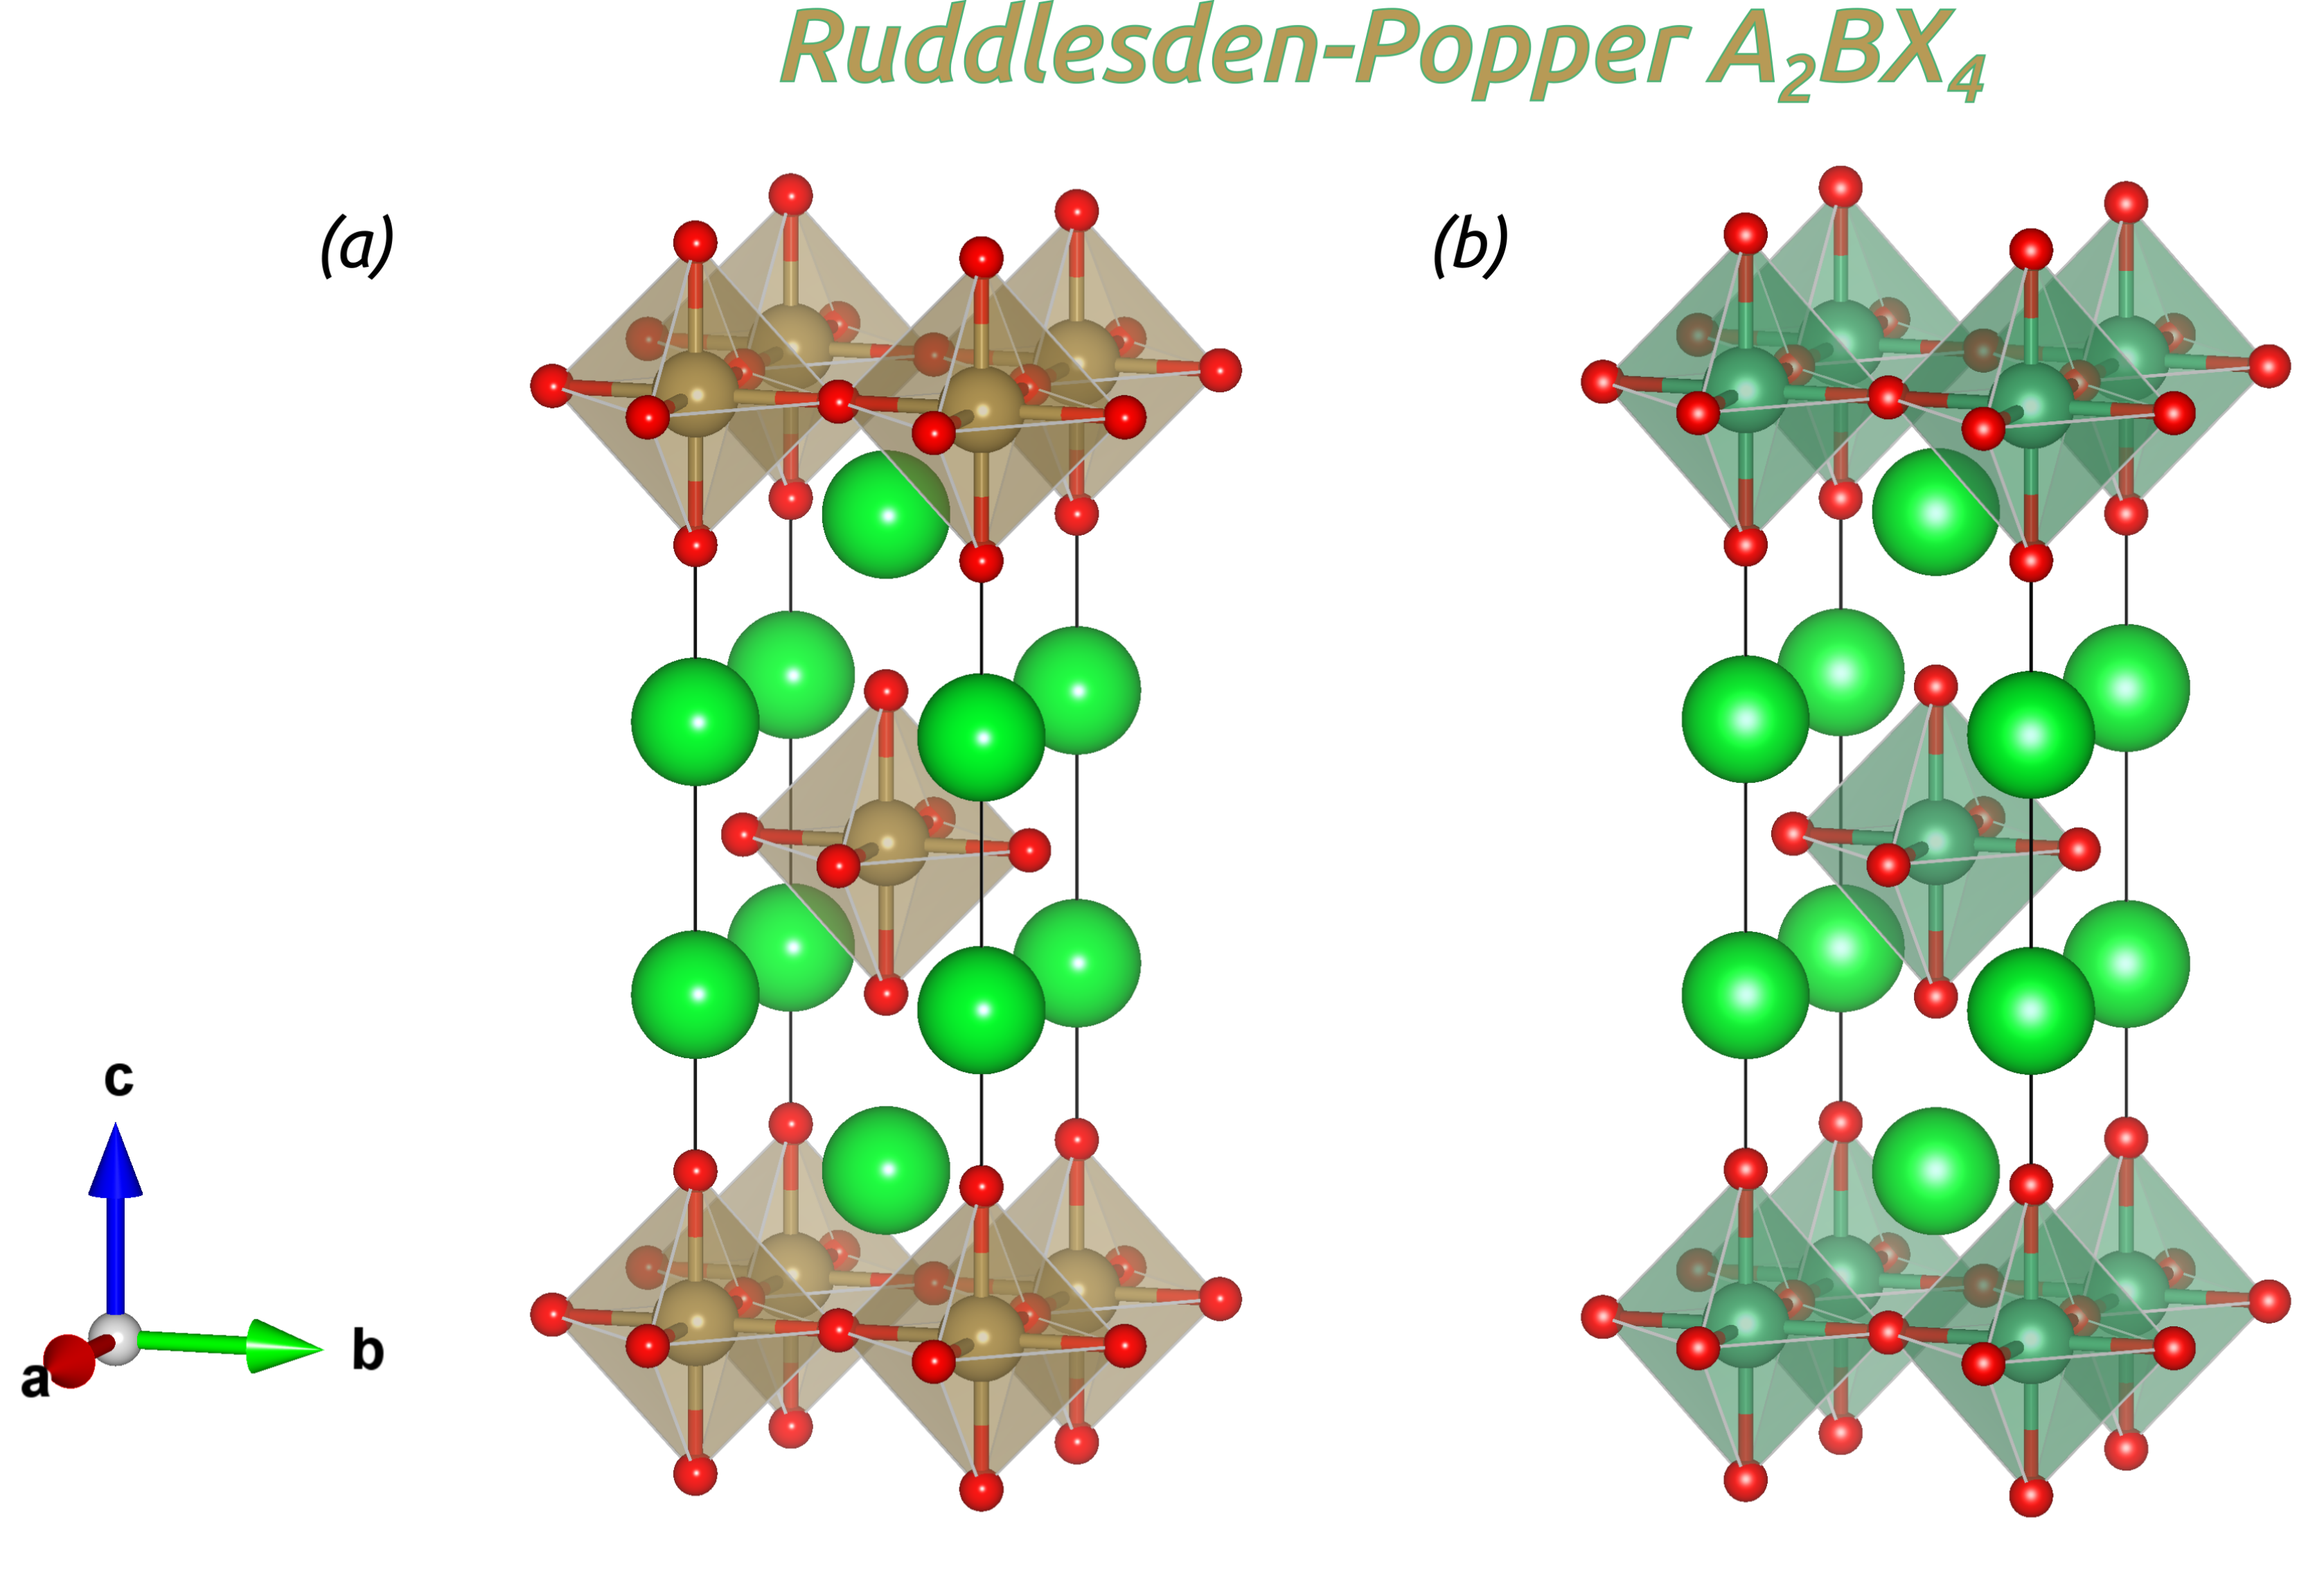
\includegraphics[width=0.6\textwidth]{Figs/rp_ta-nb.png}
    \caption{Estructuras cristalinas de la fase Ruddlesden-Popper: \textcolor{Sr}{$Sr_{2}$}\textcolor{Ta}{$Ta$}\textcolor{O}{$O_{4}$} y (b) \textcolor{Sr}{$Sr_{2}$}\textcolor{Nb}{$Nb$}\textcolor{O}{$O_{4}$}.}
    \label{Fig. rp_nb-ta}
\end{figure}

Modelar desorden en cristales es deseable debido a su estabilidad termodinámica y a propiedades sensibles al desorden.  El desorden en un cristal puede tomar varias formas: desorden dinámico \cite{Chick2009analysis}, desorden estático continuo y desorden estático discreto \cite{Muller2009structures}. Este ultimo contiene el tipo de 'desorden substitucional' \cite{Habgood2011model}, donde se substituye un anión por otro anión, lo cual hace el código \textsc{sod}\cite{Grau-Crespo2007}. Cuando se realizan substituciones isovalentes, como substituir aniones con igual oxidación como $O^{2-}$ por $S^{2-}$, trae consigo cambios sutiles a la estructura y sus propiedades. Sin embargo, la substitución de aniones aliovalentes, como $O^{2-}$ por $N^{3-}$, brindan cambios significativos en la estructura del material y sus propiedades electrónicas\cite{Roy2019}. Los oxinitruros \textsc{rp} con fórmula $Sr_{2}TaO_{3-x}N_{x}$ y $Sr_{2}NbO_{3-x}N_{x}$ preparados para substitución parcial del anión $O^{2-}$ por el anión $N^{3-}$ han recibido atención en recientes años debido a su potencial aplicación en dieléctricos, ferroeléctricos, fotocatálisis y materiales magneto-resistivos\cite{Fuertes2011}. La substitución de aniones en óxidos, sulfuros y otros materiales es comúnmente empleada para cambiar la estructura y sus propiedades dependiendo si la substitución es isovalente o aliovalente. 

\subsection{Substitución parcial x=0.5 en \textsc{rp}}

La fórmula de la fase oxinitrada \textsc{rp} con substitución parcial $x=0.5$ es: $Sr_{2}TaO_{3.5}N_{0.5}$ y  $Sr_{2}NbO_{3.5}N_{0.5}$. El nitrógeno $N^{3-}$ tiene la posibilidad de ocupar cualquier sitio cristalográfico del oxigeno $O^{2-}$ bajo la restricción de la simetría del grupo espacial $I4/mmm$ (SG. 139), esto conduce a la existencia de un numero finito de configuraciones posibles que pueden ser similares entre si debido a la simetría. El programa \textsc{sod} realiza las substituciones y define que configuraciones son independientes y que configuraciones son equivalentes a las independientes, aprovechando la simetría del cristal\cite{Grau-Crespo2007}.

\begin{figure}[H]
    \centering
    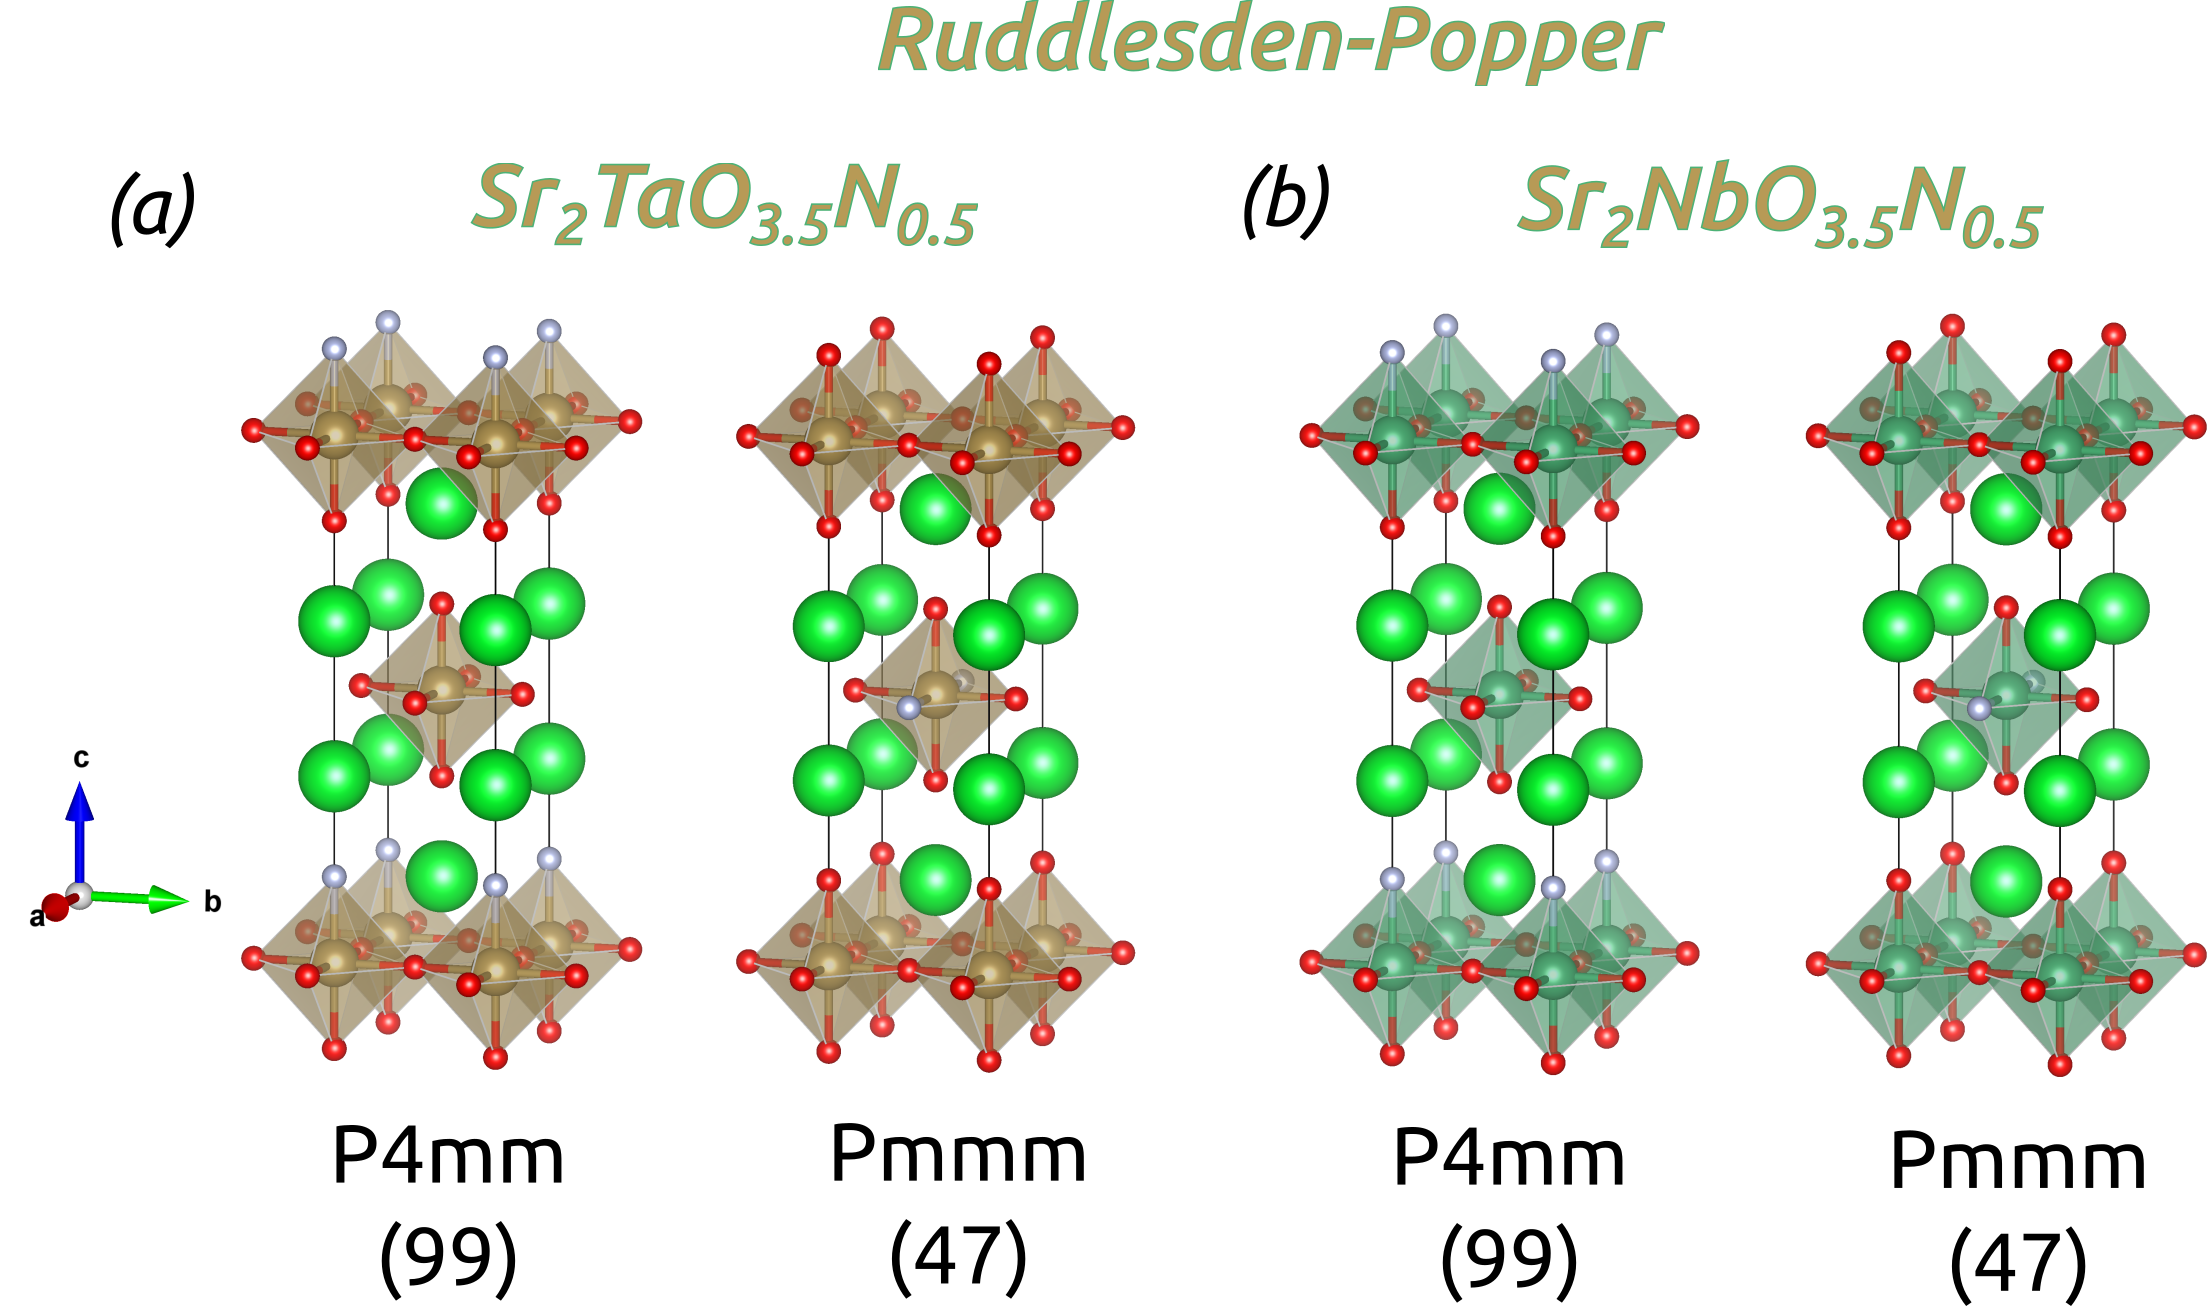
\includegraphics[width=0.7\textwidth]{Figs/rp_05.png}
    \caption{Estructuras cristalinas de la fase Ruddlesden-Popper después de substituir un oxigeno por un nitrógeno: (a) \textcolor{Sr}{$Sr_{2}$}\textcolor{Ta}{$Ta$}\textcolor{O}{$O_{3.5}$}\textcolor{N}{$N_{0.5}$} y (b) \textcolor{Sr}{$Sr_{2}$}\textcolor{Nb}{$Nb$}\textcolor{O}{$O_{3.5}$}\textcolor{N}{$N_{0.5}$}.}
    \label{Fig. rp_05}
\end{figure}

Al realizar la substitución parcial $x=0.5$ se obtienen $8$ configuraciones en total, pero solo $2$ son independientes. Este resultado es el mismo tanto para $Sr_{2}TaO_{3.5}N_{0.5}$ como para  $Sr_{2}NbO_{3.5}N_{0.5}$. Las dos configuraciones encontradas tienen grupo de simetría espacial cristalográfico diferente a la simetría inicial, esto depende del sitio que ocupen los nitrógenos en la estructura. La primera configuración de las figuras \ref{Fig. rp_05}(a) y \ref{Fig. rp_05}(b) con simetría espacial $P4mm$ (SG. 99) muestran que los nitrógeno ocupan los sitios superiores en los octaedros de las esquinas, pero el octaedro central de la celda unitaria no tiene ningún nitrógeno. 
La segunda configuración de las figuras \ref{Fig. rp_05}(a) y \ref{Fig. rp_05}(b) con simetría espacial $Pmmm$ (SG. 47) muestran una ocupación del nitrógeno tipo \emph{'trans'} en la dirección \emph{'a'} únicamente en el octaedro central, pero ninguna ocupación del nitrógeno en los octaedros de las esquinas. El poco contenido de nitrógeno muestra que no puede ocupar sitios en todos los octaedros, por esta razón las únicas dos configuraciones de esta sustitución muestran nitrógeno en capas intercaladas.

\subsection{Substitución parcial x=1.0 en \textsc{rp}}

La fórmula de la fase oxinitrada \textsc{rp} con substitución parcial $x=1.0$ es: $Sr_{2}TaO_{3}N$ y  $Sr_{2}NbO_{3}N$. En este caso, el numero de configuraciones obtenidas después de la sustitución son $28$ configuraciones en total, y solo $8$ independientes. En la figura \ref{Fig. rp_1} se muestran las $8$ configuraciones con diferente ordenamiento aniónico, tanto para \textsc{rp}-$Sr_{2}TaO_{3}N$  como para \textsc{rp}-$Sr_{2}NbO_{3}N$.

\begin{figure}[H]
    \centering
    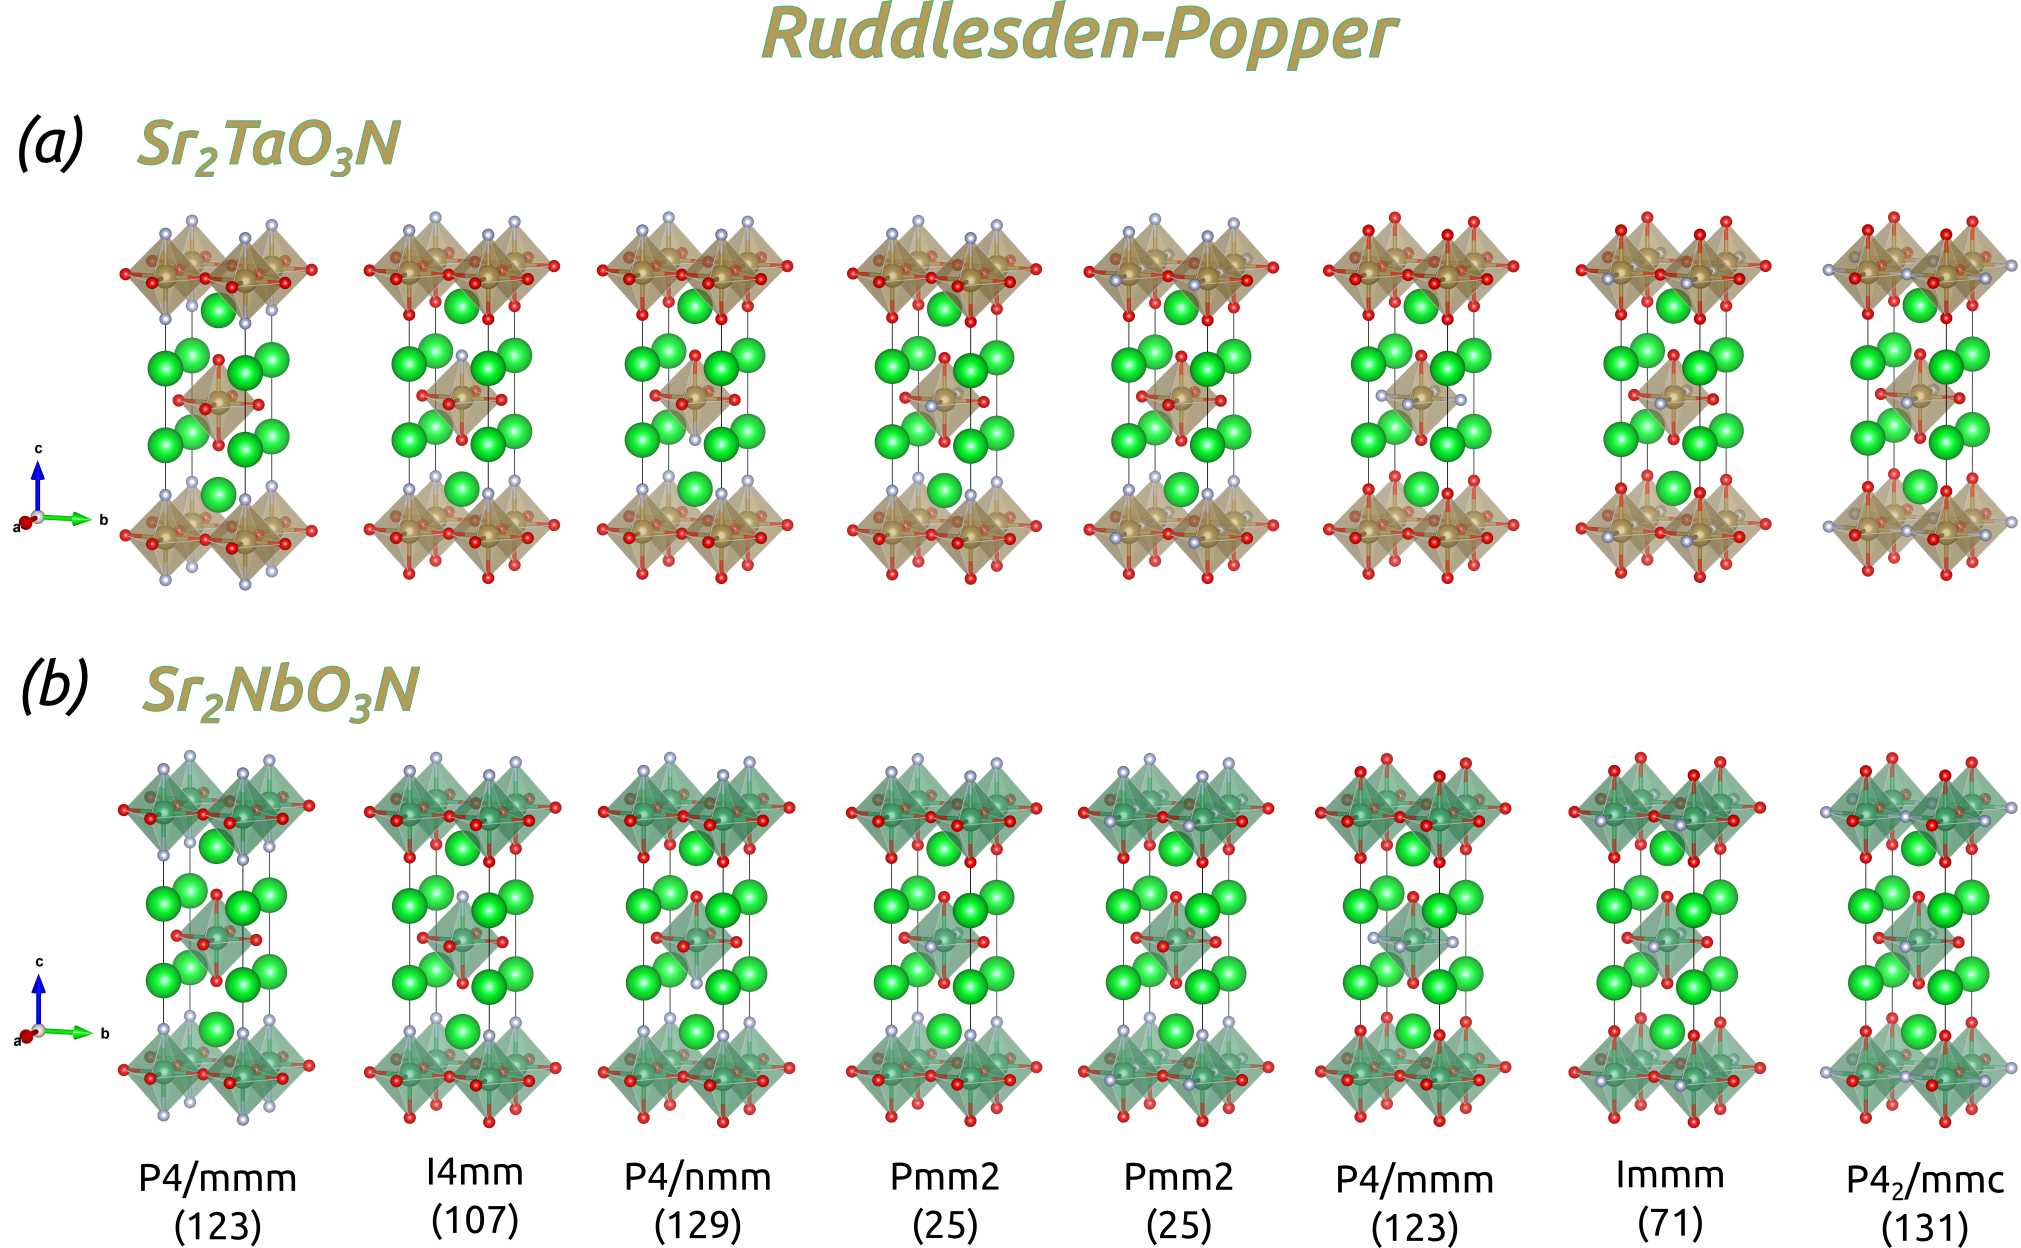
\includegraphics[width=\textwidth]{Figs/rp_1.png}
    \caption{Estructuras cristalinas de la fase Ruddlesden-Popper después de sustituir dos oxígenos por dos nitrógenos: (a) \textcolor{Sr}{$Sr_{2}$}\textcolor{Ta}{$Ta$}\textcolor{O}{$O_{3}$}\textcolor{N}{$N$} y (b) \textcolor{Sr}{$Sr_{2}$}\textcolor{Nb}{$Nb$}\textcolor{O}{$O_{3}$}\textcolor{N}{$N$}.}
    \label{Fig. rp_1}
\end{figure}

La primera configuración $P4/mmm$ (123) tiene el mismo grupo espacial que la configuración 6, pero diferente ordenamiento aniónico. La primera tiene ocupación de nitrógeno en los octaedros de las esquinas tipo \emph{trans} en la dirección \emph{'c'}, pero el octaedro central no tiene nitrógeno. Mientras que la configuración $6$ no tiene nitrógeno en los octaedro de las esquinas, pero el octaedro central evidencia una ocupación de oxigeno de tipo \emph{trans} en la dirección \emph{'c'}, es decir, los nitrógenos ocupan los sitios ecuatoriales del octaedro central.

Las configuraciones $I4mm$ (107) y $P4/nmm$ (129) tienen en común la ocupación del nitrógeno en el sitio superior del octaedro, pero con la diferencia de que el nitrógeno del octaedro central de la configuración 129 esta en el sitio inferior. Las dos configuraciones $Pmm2$ (25) tienen distintos ordenamientos aniónicos, el primero tiene $N$ en el sitio superior de los octaedros de las esquinas, mientras que el octaedro central tiene ordenamiento de $N$ tipo \emph{trans} en dirección \emph{'a'}; la segunda configuración no tiene $N$ en el octaedro central, pero tiene un ordenamiento particular tipo \emph{mer} en los octaedros de las esquinas. Las dos últimas configuraciones, $Immm$ (71) y $P4_{2}/mmc$ (131), tienen ordenamiento tipo \emph{trans} en todos sus octaedros, la configuración con grupo espacial $71$ tiene el ordenamiento de $N$ en dirección $a$, pero la configuración $131$ tienen el ordenamiento de $N$ en la dirección $b$ solo de los octaedros de las esquinas. El aumento de nitrógeno en la estructura hace que pueda ocupar mas sitios en el octaedro, haciendo que existan mas configuraciones que la substitución x=0.5.

% En todas las configuraciones presentadas no se observa ninguna relación entre el grupo espacial cristalográfico y el ordenamiento aniónico.\\

Al substituir los aniones en los sitios cristalográficas, el programa \textsc{sod} no tiene en cuenta si debe desplazar los sitios debido a las nuevas interacciones atómicas entre el metal de transición, $Ta/Nb$, y el nitrógeno, así que las estructuras deben pasar por un proceso de relajación para redefinir los sitios según las nuevas interacciones.
 % Modelo matemático del DRON
% ------------------------------------------------------------------------
% ------------------------------------------------------------------------
% ------------------------------------------------------------------------
%                                Capítulo 4
% ------------------------------------------------------------------------
% ------------------------------------------------------------------------
% ------------------------------------------------------------------------
%https://programmerclick.com/article/61381626434/
%\chapter{RELAJACIÓN ESTRUCTURAL DE LAS CONFIGURACIONES RP ENCONTRADAS}
% ------------------------------------------------------------------------.
\section{RELAJACIÓN ESTRUCTURAL DE LAS CONFIGURACIONES RP}\label{Sec. 2.2}

La relajación estructural, o también conocida como optimización, es un cálculo necesario para ajustar los sitios cristalográficos y así minimizar la energía interna de la estructura. Es decir, el cálculo desplaza los iones hasta que las fuerzas interatómicas sean casi nulas ($\sim0.02 eV$) y llegar a un estado estable. En esta sección se discuten los detalles computacionales mas relevante para el cálculo, como el parámetro de Hubbard \textsc{u} que corrige el sitio de Coulomb; además se discuten los detalles estructurales de cada configuración, como los parámetros de red, la energía de la estructura y sus cambios debido a la relajación.

\subsection{Relevantes detalles computacionales: Parámetro de Hubbard \textsc{u}}

La optimización estructural de \textsc{rp} $Sr_{2}(Ta,Nb)O_{3-x}N_{x}$(x=0.5 y 1.0) fue realizada mediante cálculos de primeros principios, con base en la teoría funcional de la densidad (\textsc{dft}) implementada en el código \textsc{vasp}\cite{urlvasp}. Se usó \textsc{vasp} debido a la alta precisión que tienen los pseudopotenciales basados en ondas planas \textsc{'paw'}, por sus siglas \textbf{P}lane \textbf{A}ugmented \textbf{W}aves. Los pseudopotenciales usados fueron \textsc{pbe}\textit{sol} dentro de la aproximación del funcional de intercambio-correlación \textsc{gga+u}. Es necesario introducir el parámetro \textsc{'u'} a los elementos que son altamente correlacionados ($3d$, $4d$, $5d$, magnéticos) como lo son los metales de transición niobio ($Nb$) y Tántalo ($Ta$), esto corrige la correlación a través de introducir un termino adicional en el hamiltoniano. El término de la corrección de Hubbard \textsc{'u'} entra como una energía en los orbitales, corrige la fuerza de las interacciones en el sitio de Coulomb, corrige los orbitales y la separación entre ellos (Liechtenstein\cite{Lichtenstein1995StrongOrdering}).

Los sistemas correlacionados están mal descritos por los cálculos de \textsc{dft}\cite{Tolba2018}, la manera estándar como calcula la energía no es suficiente, así que el parámetro \textsc{u} corrige la energía de correlación. A menudo, el valor \textsc{u} no se conoce y prácticamente se modifica semi-empíricamente para hacer buenos resultados computacionales en base a datos experimentales. En la literatura se encuentran varios ejemplos que muestran la relación entre el parámetro \textsc{u} y las propiedades físicas predichas:

\begin{itemize}
    \item En el estudio teórico del material $M_{3}O_{4}(M=V, Cr, Mn, Fe, Co, Ni, Cu)$ hecho por Wang et. al. \cite{Wang2006} identifican dos contribuciones al error en las energías de oxidación cuando usan el enfoque \textsc{gga}: La primera contribución se origina en la sobre-estimación del enlace en la molécula de $O_{2}$; el segundo error está relacionado con el error de correlación en orbitales $3d$,  lo que resulta en una sobre-estimación de las energías de oxidación. El enfoque \textsc{gga+u} elimina el error del enlace de $O_{2}$, permitiendo abordar los efectos de correlación en los metales de transición $3d$. Se han utilizado una variedad de valores de \textsc{u} que van de $2$ a $6 eV$ para las propiedades, incluidas la estructura de bandas, la energía de oxidación y los parámetros estructurales \cite{Wang2006}.% La banda prohibida calculada en la aproximación de gradiente generalizada (GGA) + U concuerda bien con el valor experimental de 1,6 eV. Por otro lado, el valor calculado utilizando el híbrido funcional PBE0 (3,42 eV) está muy sobreestimado, debido a que se descuida el problema de apantallamineto de la aproximación de Hartree-Fock [25]. 
    \item En materiales con metales orgánicos (\textsc{mof}), por sus siglas en inglés '\textsc{M}etal \textsc{O}rganics \textsc{F}ramework', investigado por Mann et. al. \cite{Mann2016}, muestran que la energía de enlace de $MO_{2}$ en $M-MOF-74 (M=Ti,V,Cr,Mn,Fe,Co,Ni,Cu)$ crece linealmente con el valor de Hubbard \textsc{u}, se desplaza $0,041  eV$ sobre el rango de $U = 0-5,4  eV$. Para el caso del cobalto $Co$, los parámetros de red coinciden con el experimento por el hecho de que la longitud del enlace $Co-O$ disminuye con \textsc{u}, el parámetro localiza los estados $d$ de $Co$ lo que permite que la molécula de $CoO_{2}$ se acerque más al sitio del \textsc{mof}, aumentando la contribución electrostática a la energía de enlace \cite{Mann2016}.
     
    \item Dentro del estudio de $BiMnO_{3}$ realizado por Boukhvalov et. al. \cite{Boukhvalov2010} señalan la desestimación de \textsc{gga} en las distorsiones Jahn-Teller. Como los octaedros $MnO_{6}$ tiene distorsiones fuertes, utilizan la teoría funcional de la densidad con la corrección de Coulomb \textsc{dft+u}. El estudio mostró que un valor de $U=2 eV$ hace que los resultados se aproximen a los datos experimentales. Además, para valores grandes de \textsc{u} ($4$ y $8 eV$) disminuye la hibridación $3d-2p$, por ende, incrementa la distancia del enlace $Mn-O$ disminuyendo los efectos de enlace. \cite{Boukhvalov2010}.
    
    \item La \href{https://pubs.acs.org/doi/suppl/10.1021/acsmaterialslett.9b00088/suppl_file/tz9b00088_si_001.pdf}{información suplementaria} del trabajo de Ouhbi y Ulrich \cite{Ulrich2019} muestra la evolución de la densidad de estados con el aumento del parámetro \textsc{u}. Se observa un cambio significativo a partir de $U=4  eV$ para el material $SrTaO_{2}N$, además de reportar cambios en la brecha entre la banda de valencia y la banda de conducción de la estructura de bandas electrónica.
\end{itemize}

%\textsc{dft+u} ha demostrados ser simple en términos de formulación teórica e implementación practica con un considerable bajo costo computacional\cite{Tolba2018}. 
En general, cuanto más localizado es un sistema, más sensible es al valor de \textsc{u} \cite{Tolba2018}. En el caso de esta investigación, la corrección se realiza para el niobio $Nb$ y el tántalo $Ta$ con un valor de $U=4.0 eV$. La comparación entre la relajación estructural usando \textsc{dft} y \textsc{dft+u} se presenta en el anexo \ref{anexoB}. Además, se agregó la energía de corte que controla el numero de ondas planas (\textsc{paw}), con un valor de $550 eV$; en la malla de puntos $k$ de la zona de Brillouin se aplica el método Monkhorst-Pack \cite{Monkh1976} para discretizar el espacio y conocer el numero de puntos que definen correctamente el sistema, en este caso se uso una malla de $8\times8\times4$. 
 
Esta sección empieza con el análisis composicional de las estructuras oxinitradas, luego se abordara el análisis energético de cada configuración para dos tipos de concentración de nitrógeno: $x=0.5$ y $x=1.0$.

\subsection{Diagrama de concentraciones aniónicas}

En un diagrama de concentraciones aniónicas, ó convex hull, se involucra la diferencia de energía respecto a las estructuras puras en función de las concentraciones aniónicas $x=0.0$, $x=0.5$, $x=1.0$ y $x=4.0$, como se muestra en la figura \ref{Fig. concentraciones-totales}. Las estructuras puras de óxido $Sr_{2}(Ta,Nb)O_{4}$ y nitruros $Sr_{2}(Ta,Nb)N_{4}$ son usadas como referencia para comparar la energía de las concentraciones $x=0.5$ y $x=1.0$.

\begin{figure}[H]
    \centering
    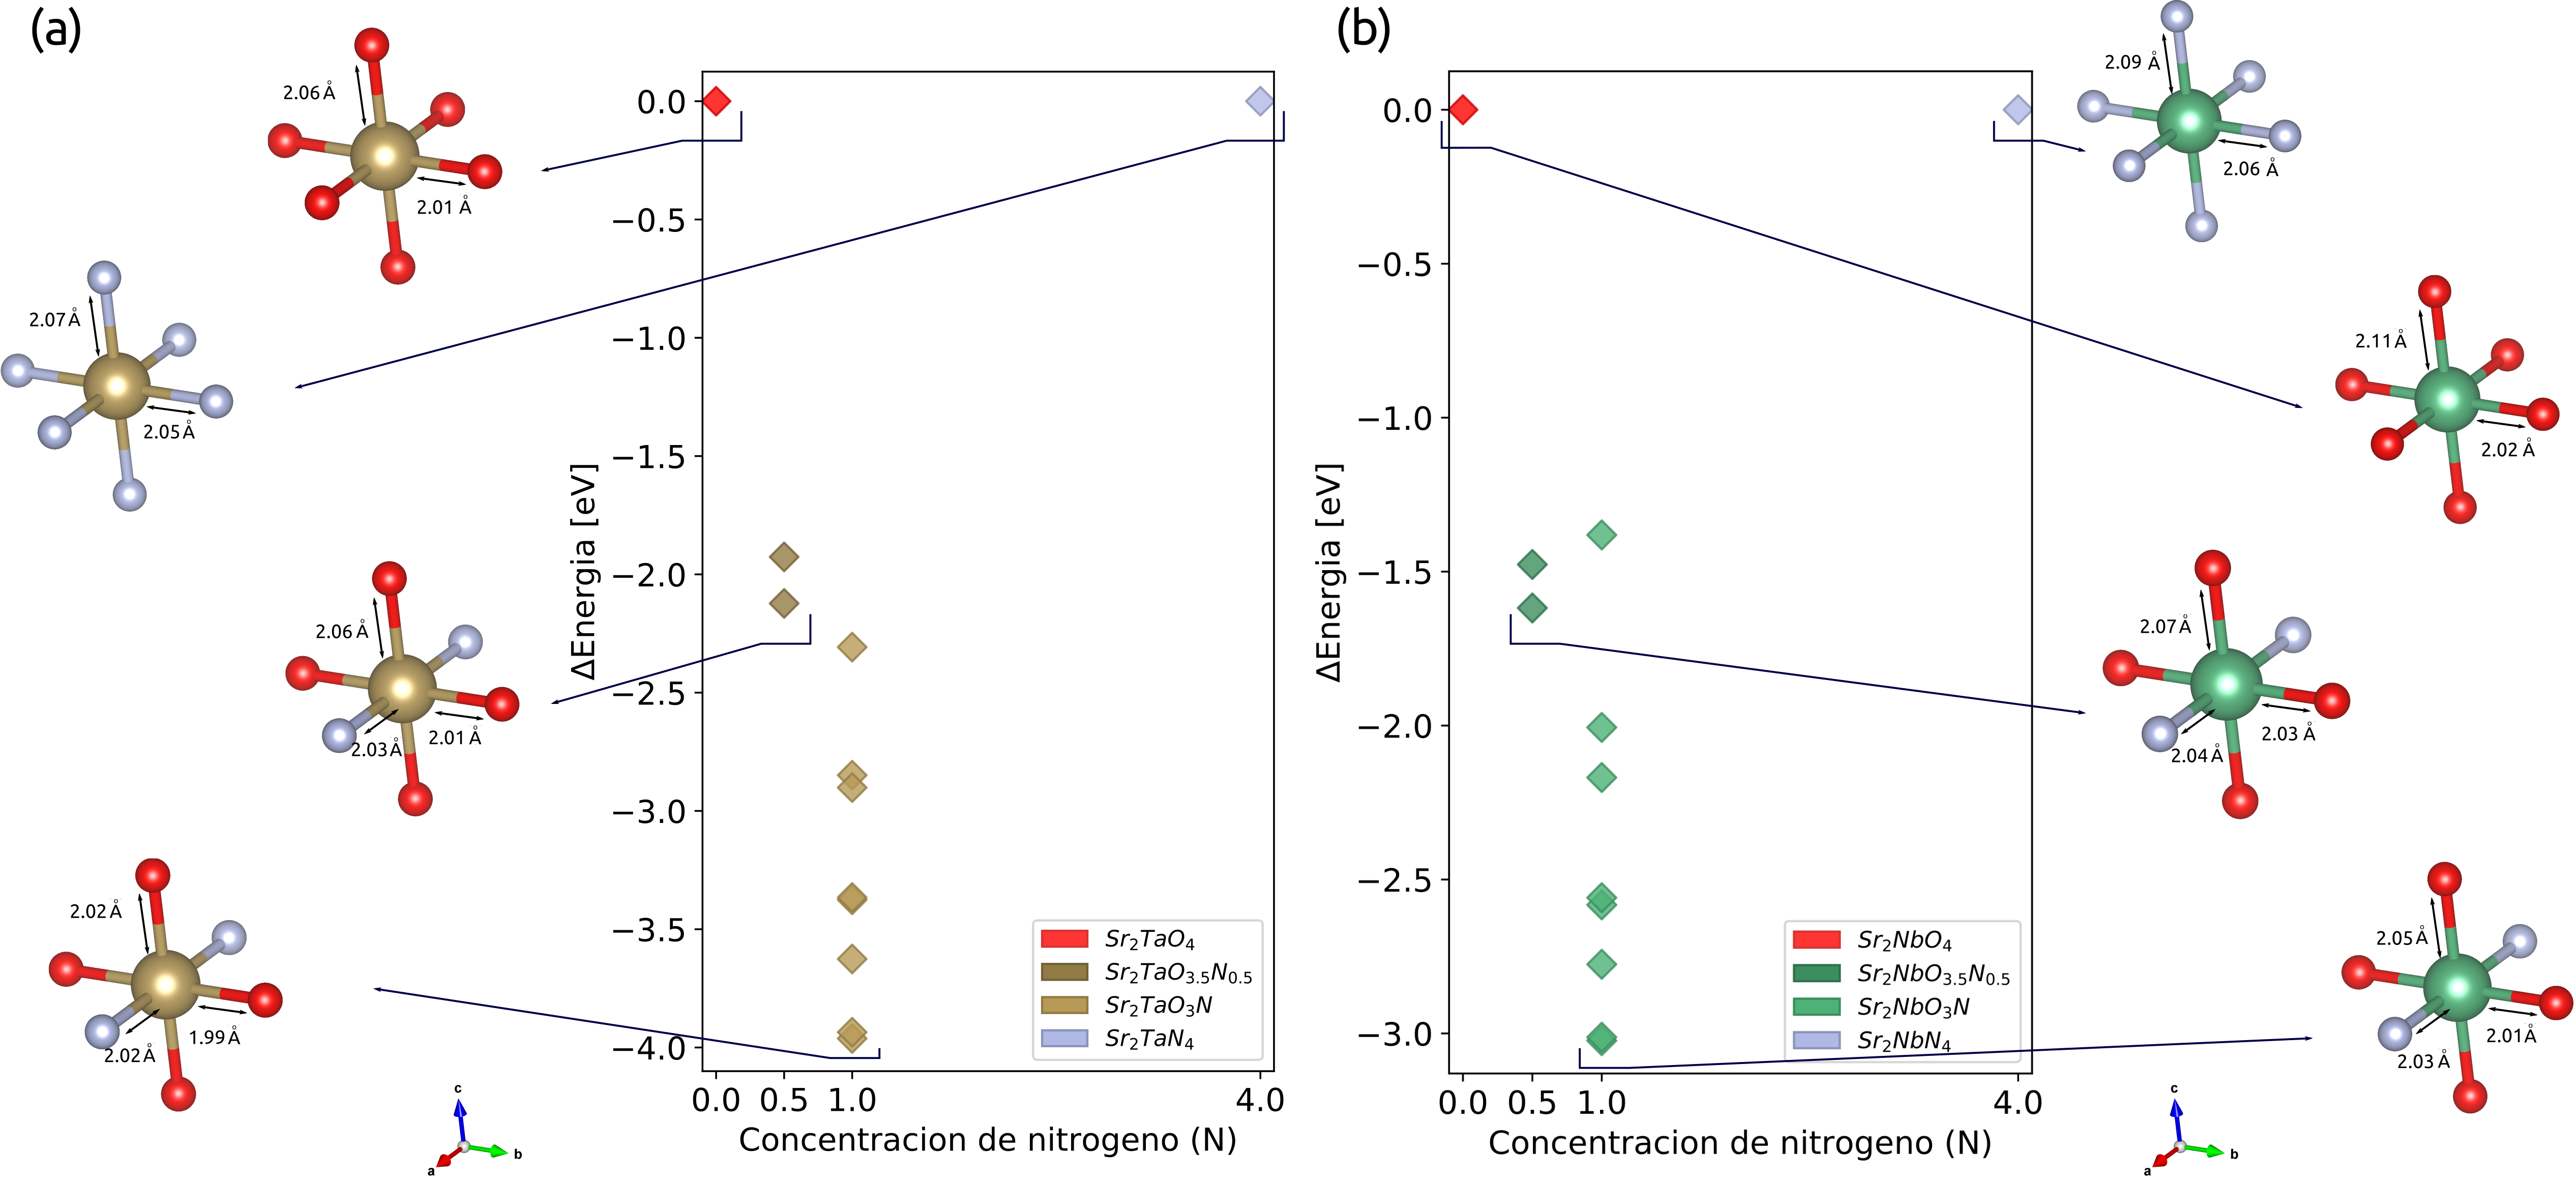
\includegraphics[width=\textwidth]{Figs/convex_hull.png}
    \caption{Diagrama de concentraciones de oxígeno y nitrógeno para $x=0.5$ y $x=1.0$ en las estructuras cristalinas Ruddlesden-Popper (a) $Sr_{2}TaO_{4-x}N_{x}$ y (b) $Sr_{2}NbO_{4-x}N_{x}$.}
    \label{Fig. concentraciones-totales}
\end{figure}

En cada concentración las configuraciones mas favorables son las de menor energía. Al observar la concentración $x=0.5$ se encuentra la configuración mas favorable en $-2.12 eV$ y $-1.62 eV$ para $Sr_{2}TaO_{3.5}N_{0.5}$ y $Sr_{2}NbO_{3.5}N_{0.5}$ respectivamente. En la concentración $x=1.0$ se encuentra la configuración mas favorable en $-3.96 eV$ y $-3.02 eV$ para $Sr_{2}TaO_{3}N$ y $Sr_{2}NbO_{3}N$ respectivamente. Las configuraciones inestables siempre aparecerán por encima de las configuraciones favorables. Las configuraciones con concentración x=1.0 son mas estables comparadas con las configuraciones con concentración x=0.5 debido a un mayor contenido de nitrógeno en la estructura, mostrando que el nitrógeno si reduce las energía estructural comparada con los oxidos y los nitruros puros.

La distancia de los enlaces $(Ta,Nb)-O$ y $(Ta,Nb)-N$ se mantienen para ambos compuestos, entre $2.02  \si{\angstrom}$ y $2.07  \si{\angstrom}$ como se reporta experimentalmente \cite{Diot1999CrystalN,Tobias2004,Clarke2002,Ebbinghaus2004PowderK,Tobias2010ChemInform2.}. Las distancias son muy similares ya que el nitrógeno tiene un radio iónico ligeramente mayor en comparación con el oxigeno, pero esto es compensado con un acortamiento del enlace asociado a una mayor covalencia con el metal de transición \cite{Yang2011,Ebbinghaus2004PowderK}.  El efecto combinado de los enlaces $(Ta,Nb)-O$ y $(Ta,Nb)-N$ y la distribución no uniforme de $N/O$ rompen la simetría del cristal, por lo que es común que las estructuras oxinitradas caigan a una simetría mas baja que $I4/mmm(139)$. Para continuar con el análisis, la siguiente sección presenta el acoplamiento entre la energía estructural de cada configuración y los ordenamientos aniónicos obtenidos en la substitución aniónica.

%. P. Ong, L. Wang, B. Kang, G. Ceder., The Li-Fe-P-O2 Phase Diagram from First Principles Calculations, Chemistry of Materials, vol. 20, Mar. 2008, pp. 1798-1807.
%S.P. Ong, A. Jain, G. Hautier, B. Kang, and G. Ceder, Thermal stabilities of delithiated olivine MPO4 (M=Fe, Mn) cathodes investigated using first principles calculations, Electrochemistry Communications, vol. 12, 2010, pp. 427-430.
 
%[REF: Vaadium oxynitrides as stable catalysts...(Pan)]
 
\subsection{Energía de las configuraciones $Sr_{2}(Ta,Nb)O_{3.5}N_{0.5}$}

La sustitución aniónica x=0.5 resultó en dos configuraciones con diferente ordenamiento aniónico. La energía estructural de cada configuración se muestra en la figura \ref{Fig. 35u-rp}.

\begin{figure}[H]
    \centering
    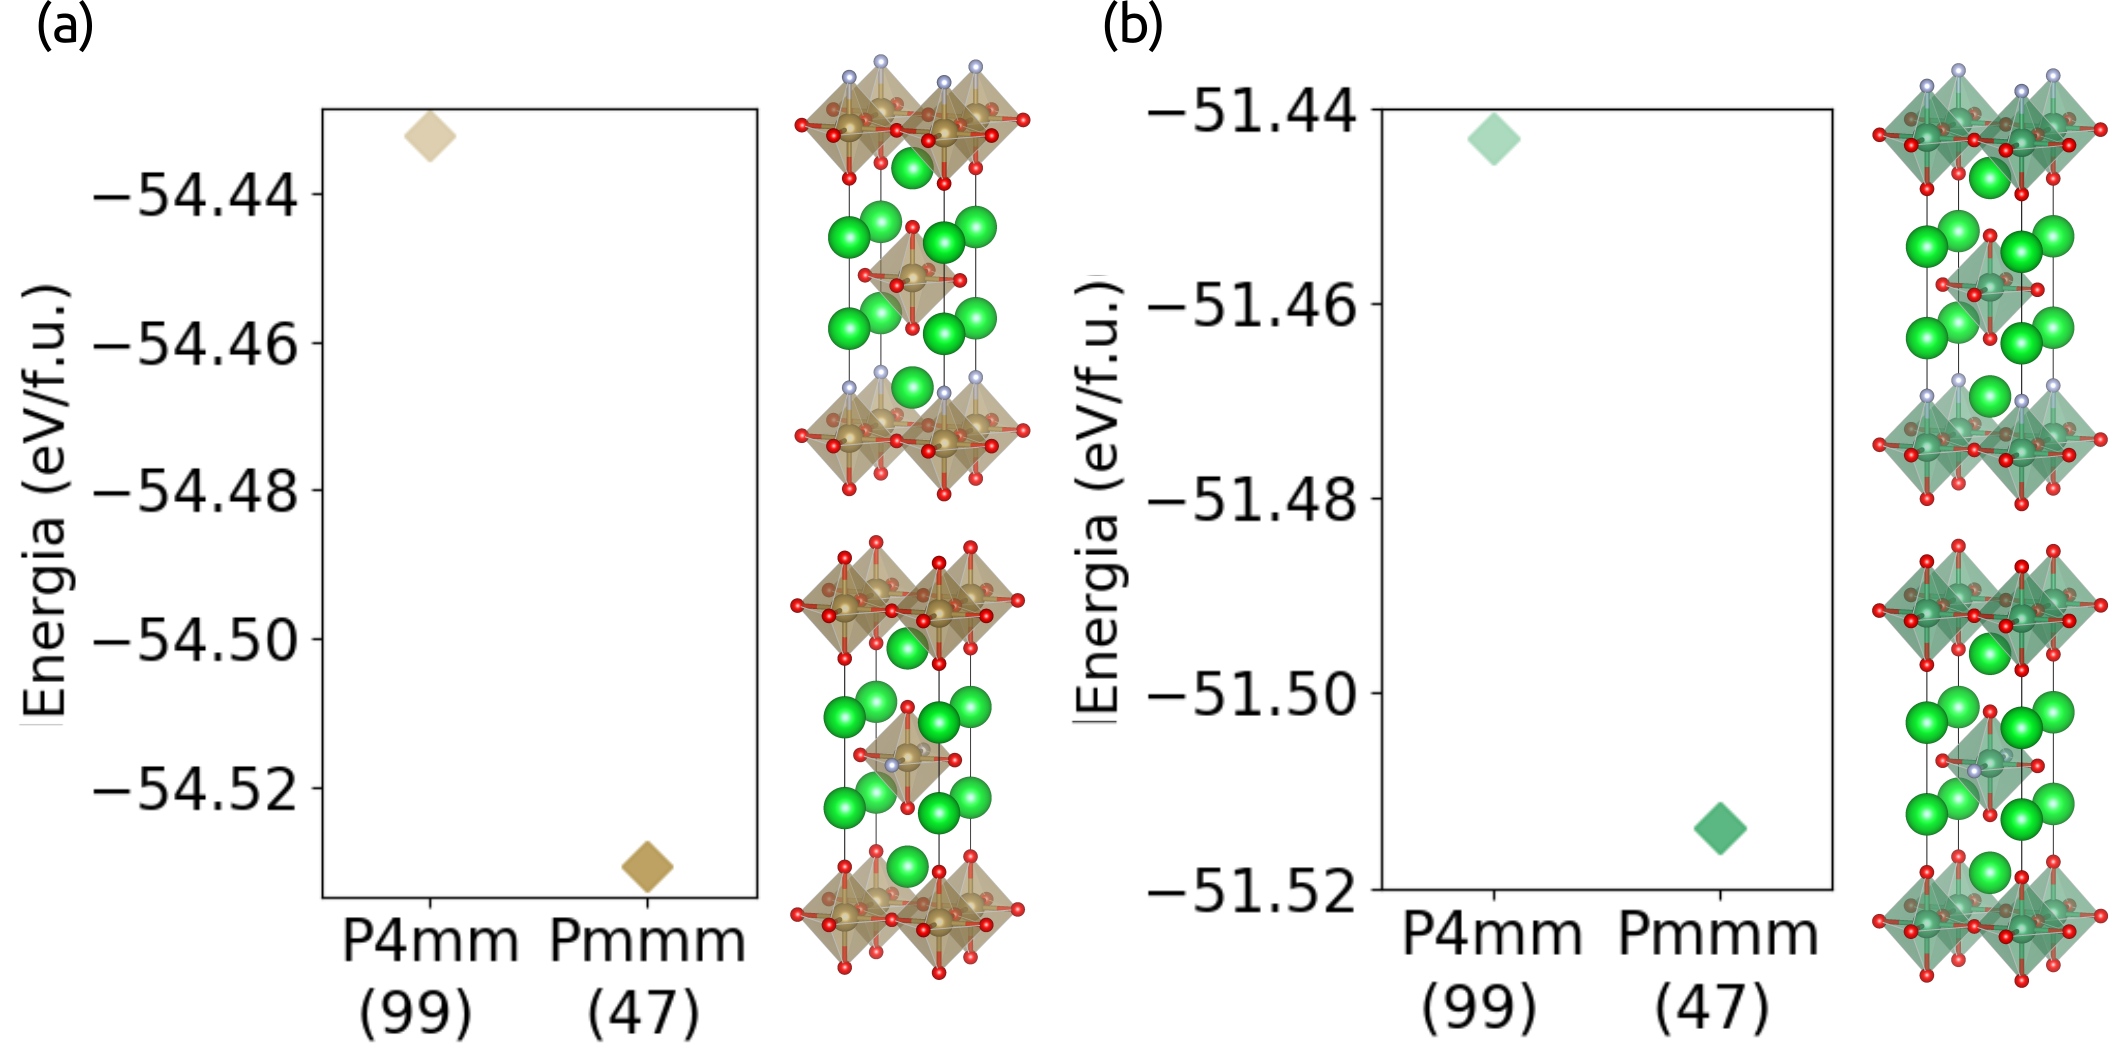
\includegraphics[width=\textwidth]{Figs/35u-rp.png}
    \caption{Energía estructural de la concentración $x=0.5$ en función del grupo de simetría espacial para las configuraciones \textsc{rp} (a) $Sr_{2}TaO_{3.5}N_{0.5}$ y (b) $Sr_{2}NbO_{3.5}N_{0.5}$.}
    \label{Fig. 35u-rp}
\end{figure}

Las estructuras de mínima energía tienen simetría de grupo espacial $Pmmm(47)$ con un valor de $-54.53 eV$ y $-51.51  eV$ respectivamente. Esta configuración favorable exhibe un ordenamiento aniónico \emph{trans} en el octaedro central, pero los octaedros de las esquinas contienen únicamente oxígeno. Esto es debido al poco contenido de nitrógeno introducido en las estructuras, el nitrógeno se sitúa en un solo sitio cristalográfico que, por simetría, se situó en el sitio ecuatorial de manera \emph{trans}. Igualmente pasa con la configuración $P4mm(99)$, el nitrógeno se ubica en el sitio superior del octaedro. La energía de la configuración \emph{trans-}$47$ indica que los nitrógenos prefieren situarse en sitios ecuatoriales que en sitios axiales del octaedro.

Los parámetros de red de la configuración ($47$)-$Sr_{2}TaO_{3.5}N_{0.5}$ son $a=4.06508 \si{\angstrom}$, $b=4.03416 \si{\angstrom}$ y $c=12.56372 \si{\angstrom}$, $\alpha=\beta=\gamma=90^{\circ}$, y volumen $206.034796 \left[\si{\angstrom}^{3}\right]$,  lo parámetros de red de la configuración ($47$)-$Sr_{2}NbO_{3.5}N_{0.5}$ son $a=4.09052$, $b=4.07287 \si{\angstrom}$ y $c=12.56518 \si{\angstrom}$, $\alpha=\beta=\gamma=90^{\circ}$, y volumen $209.337701  \si{\angstrom}^{3}$. Comparando estos parámetro de red con las estructuras de óxidos puros, el parámetro en \emph{'a'} aumenta $\sim0.04  \si{\angstrom}$, mientras que en la dirección \emph{'c'} el parámetro de red disminuye $\sim0.1 \si{\angstrom}$.

\subsection{Energía de las configuraciones $Sr_{2}(Ta,Nb)O_{3}N$}

La sustitución aniónica x=1.0 resultó en ocho configuraciones con diferente ordenamiento aniónico. La energía estructural de cada configuración se muestra en la figura \ref{Fig. rp_ta-nb_energy}.

\begin{figure}[H]
    \centering
    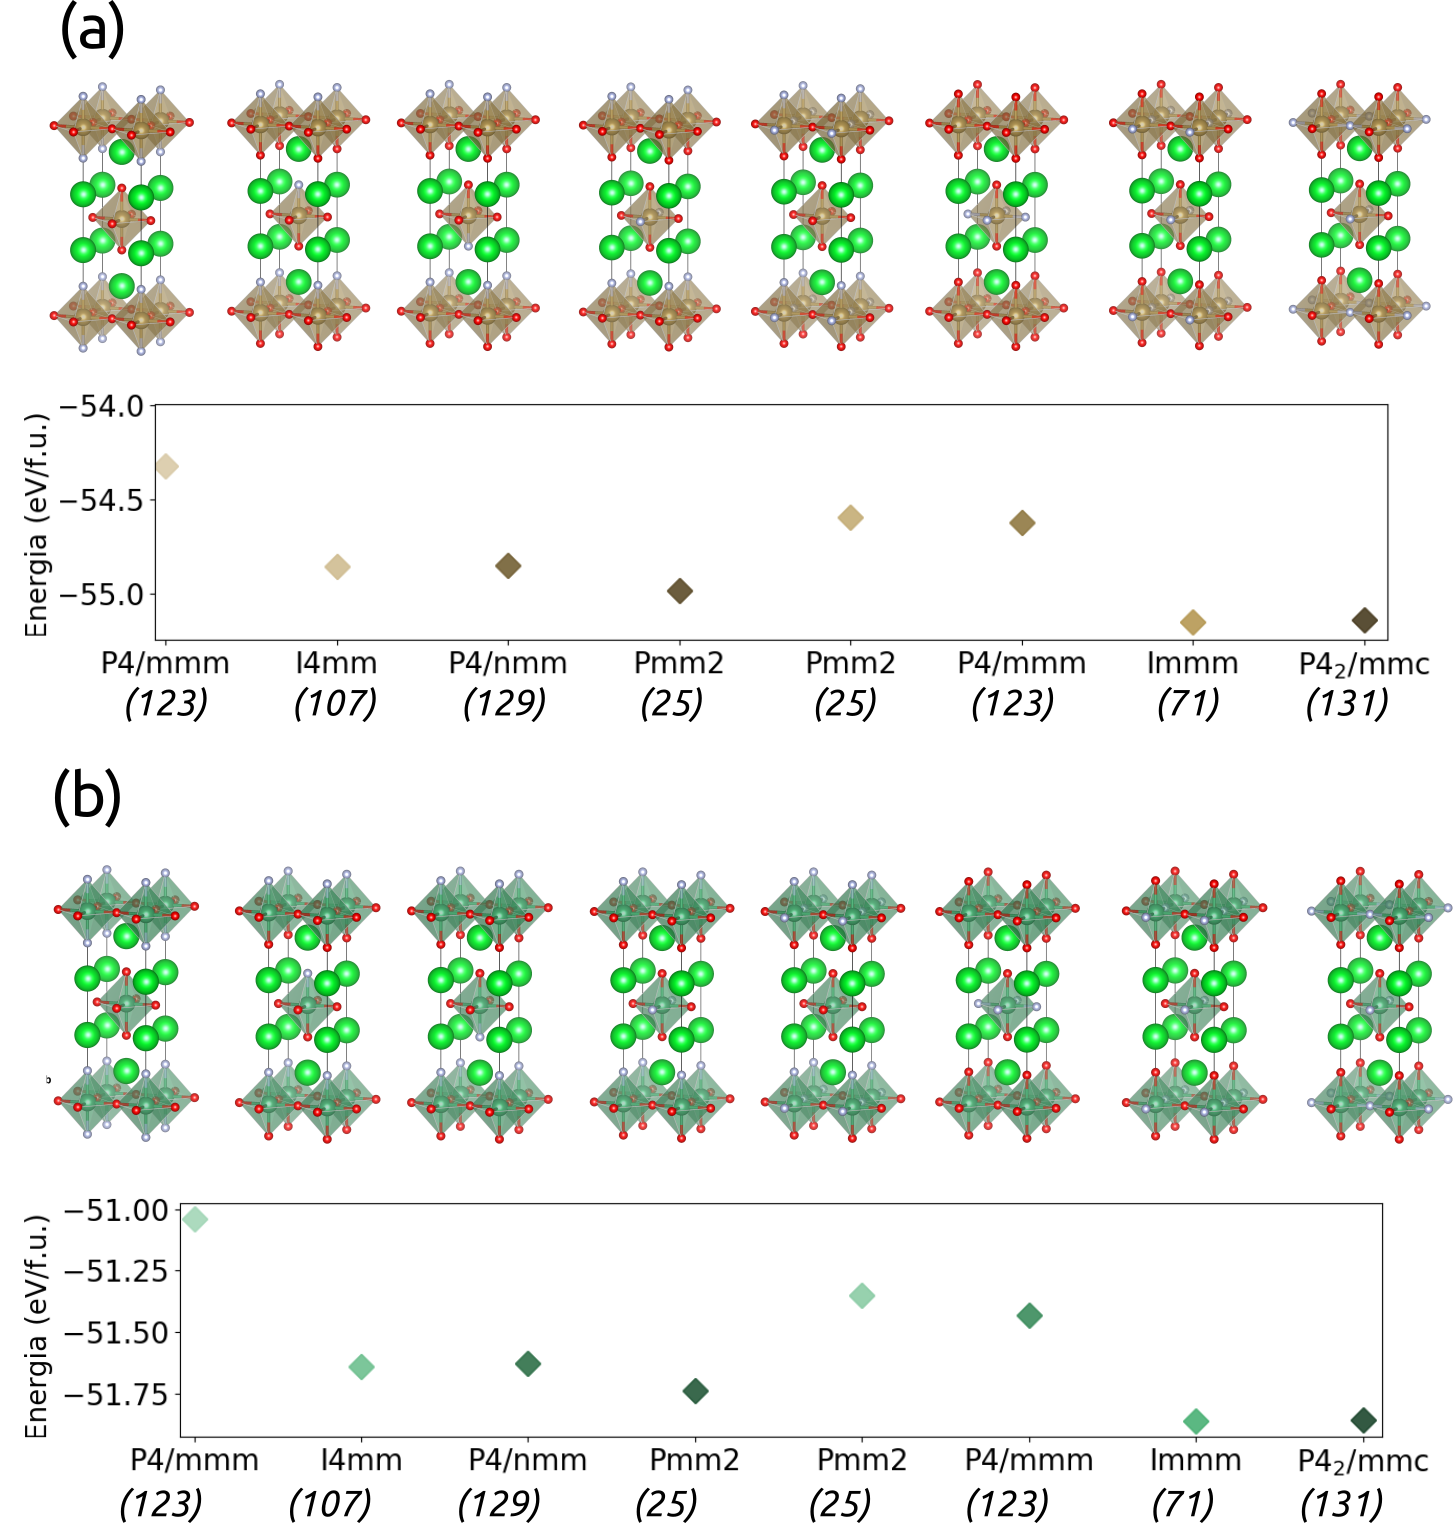
\includegraphics[width=\textwidth]{Figs/rp_ta--nb_U.png}
    \caption{Energía estructural de la concentración $x=1.0$ en función del grupo de simetría espacial para las configuraciones \textsc{rp} (a) $Sr_{2}TaO_{3}N$ y (b) $Sr_{2}NbO_{3}N$.}
    \label{Fig. rp_ta-nb_energy}
\end{figure}

Las configuraciones menos favorable están en el rango de $-54.25 eV$ a $-54.75 eV$, y $-51.00 eV$ a $-51.50 eV$ para $Sr_{2}TaO_{3}N$ y  $Sr_{2}NbO_{3}N$, respectivamente. En este rango hay tres configuraciones con grupo espacial (123), (25), (123), y presentan la particularidad de que son configuraciones donde no hay nitrógeno en algún octaedro, es decir el nitrógeno se alterna capa a capa en la perovskita \textsc{rp}, alcanzando energías iguales a las configuraciones $Sr_{2}(Ta,Nb)O_{3.5}N_{0.5}$. Esto indica que el nitrógeno debe ocupar todos los octaedros de la celda unitaria para lograr una menor energía. Las configuraciones no tan favorables están en el rango de $-54.27$ a $-55.00 eV$, y $-51.50 eV$ a $-51.75 eV$ para $Sr_{2}TaO_{3}N$ y  $Sr_{2}NbO_{3}N$, respectivamente. En este rango hay tres configuraciones con grupo espacial (107), (129), (25), presentan orden de aniones axial en todos sus octaedros. La configuración de mínima energía tienen simetría de grupo espacial $Immm(71)$ con un valor de $-55.15  eV$ y $-51.86  eV$ para $Sr_{2}TaO_{3}N$ y  $Sr_{2}NbO_{3}N$,s respectivamente. Esta configuración favorable exhibe un ordenamiento aniónico \emph{trans} con dirección \emph{'a'} en sus octaedros, todos sobre el sitio ecuatorial. La configuración $P4_{2}/mmc(131)$ también exhibe ordenamiento \emph{trans}, unas capas en dirección \emph{'a'} y otras capas en dirección \emph{'b'}, lo que la diferencia con la configuración $(71)$. Los parámetros de red de la configuración ($71$)-$Sr_{2}TaO_{3}N$ son $a=4.07855 \si{\angstrom}$, $b=4.01907 \si{\angstrom}$ y $c=12.60903 \si{\angstrom}$, $\alpha=\beta=\gamma=90^{\circ}$, y volumen $206.687252\si{\angstrom}^{3}$,  lo parámetros de red de la configuración ($71$)-$Sr_{2}NbO_{3}N$ son $a=4.08308$, $b=4.05652 \si{\angstrom}$ y $c=12.62466 \si{\angstrom}$, $\alpha=\beta=\gamma=90^{\circ}$, y volumen $209.1035  \si{\angstrom}^{3}$. Comparando estos parámetro de red con las estructuras de óxidos puros, el parámetro en \emph{'a'} aumenta $\sim0.04  \si{\angstrom}$, siendo esta la dirección del enlace $(Ta,Nb)-N$, es decir la dirección del orden aniónico \emph{trans}, mientras que en la dirección \emph{'b'}, el parámetro de red disminuye $\sim0.01 \si{\angstrom}$.

Se observa que las configuraciones mas favorables tienen ordenamiento aniónico \emph{trans}, tanto para la estructura oxinitrada \textsc{rp-}$Sr_{2}(Ta,Nb)O_{3}N$ como para  \textsc{rp-}$Sr_{2}(Ta,Nb)O_{3.5}N_{0.5}$. La conectividad de los aniones ecuatoriales requiere que cada anión esté vinculado a dos sitios del metal de transición \cite{Harada2019}, lo que solo deja dos ordenamientos posibles: \emph{cis} y \emph{trans}. Aunque en el estudio no se encontró orden de aniones \emph{cis}, y debido a los reportes experimentales y computacionales sobre una posible configuración favorable en oxinitruros con ordenamiento aniónico \emph{cis} \cite{Masubuchi2013SynthesisCeramics,Yang2011,Harada2019, Bouri2018}, es necesario buscar este ordenamiento en una celda unitaria mas grande.

\subsection{Caso especial: Configuración \emph{cis} con concentración x=1.0}

Para el estudio de la configuración \emph{cis}, se crea una supercelda con una rotación de $45^{\circ}$. Se obtuvieron 3 configuraciones con ordenamiento \emph{cis} en el plano para la concentración $x=1.0$ en ambos compuestos. La energía estructural de cada una de estas configuraciones se muestra en la figura \ref{Fig. rp_cis}.

\begin{figure}[H]
    \centering
    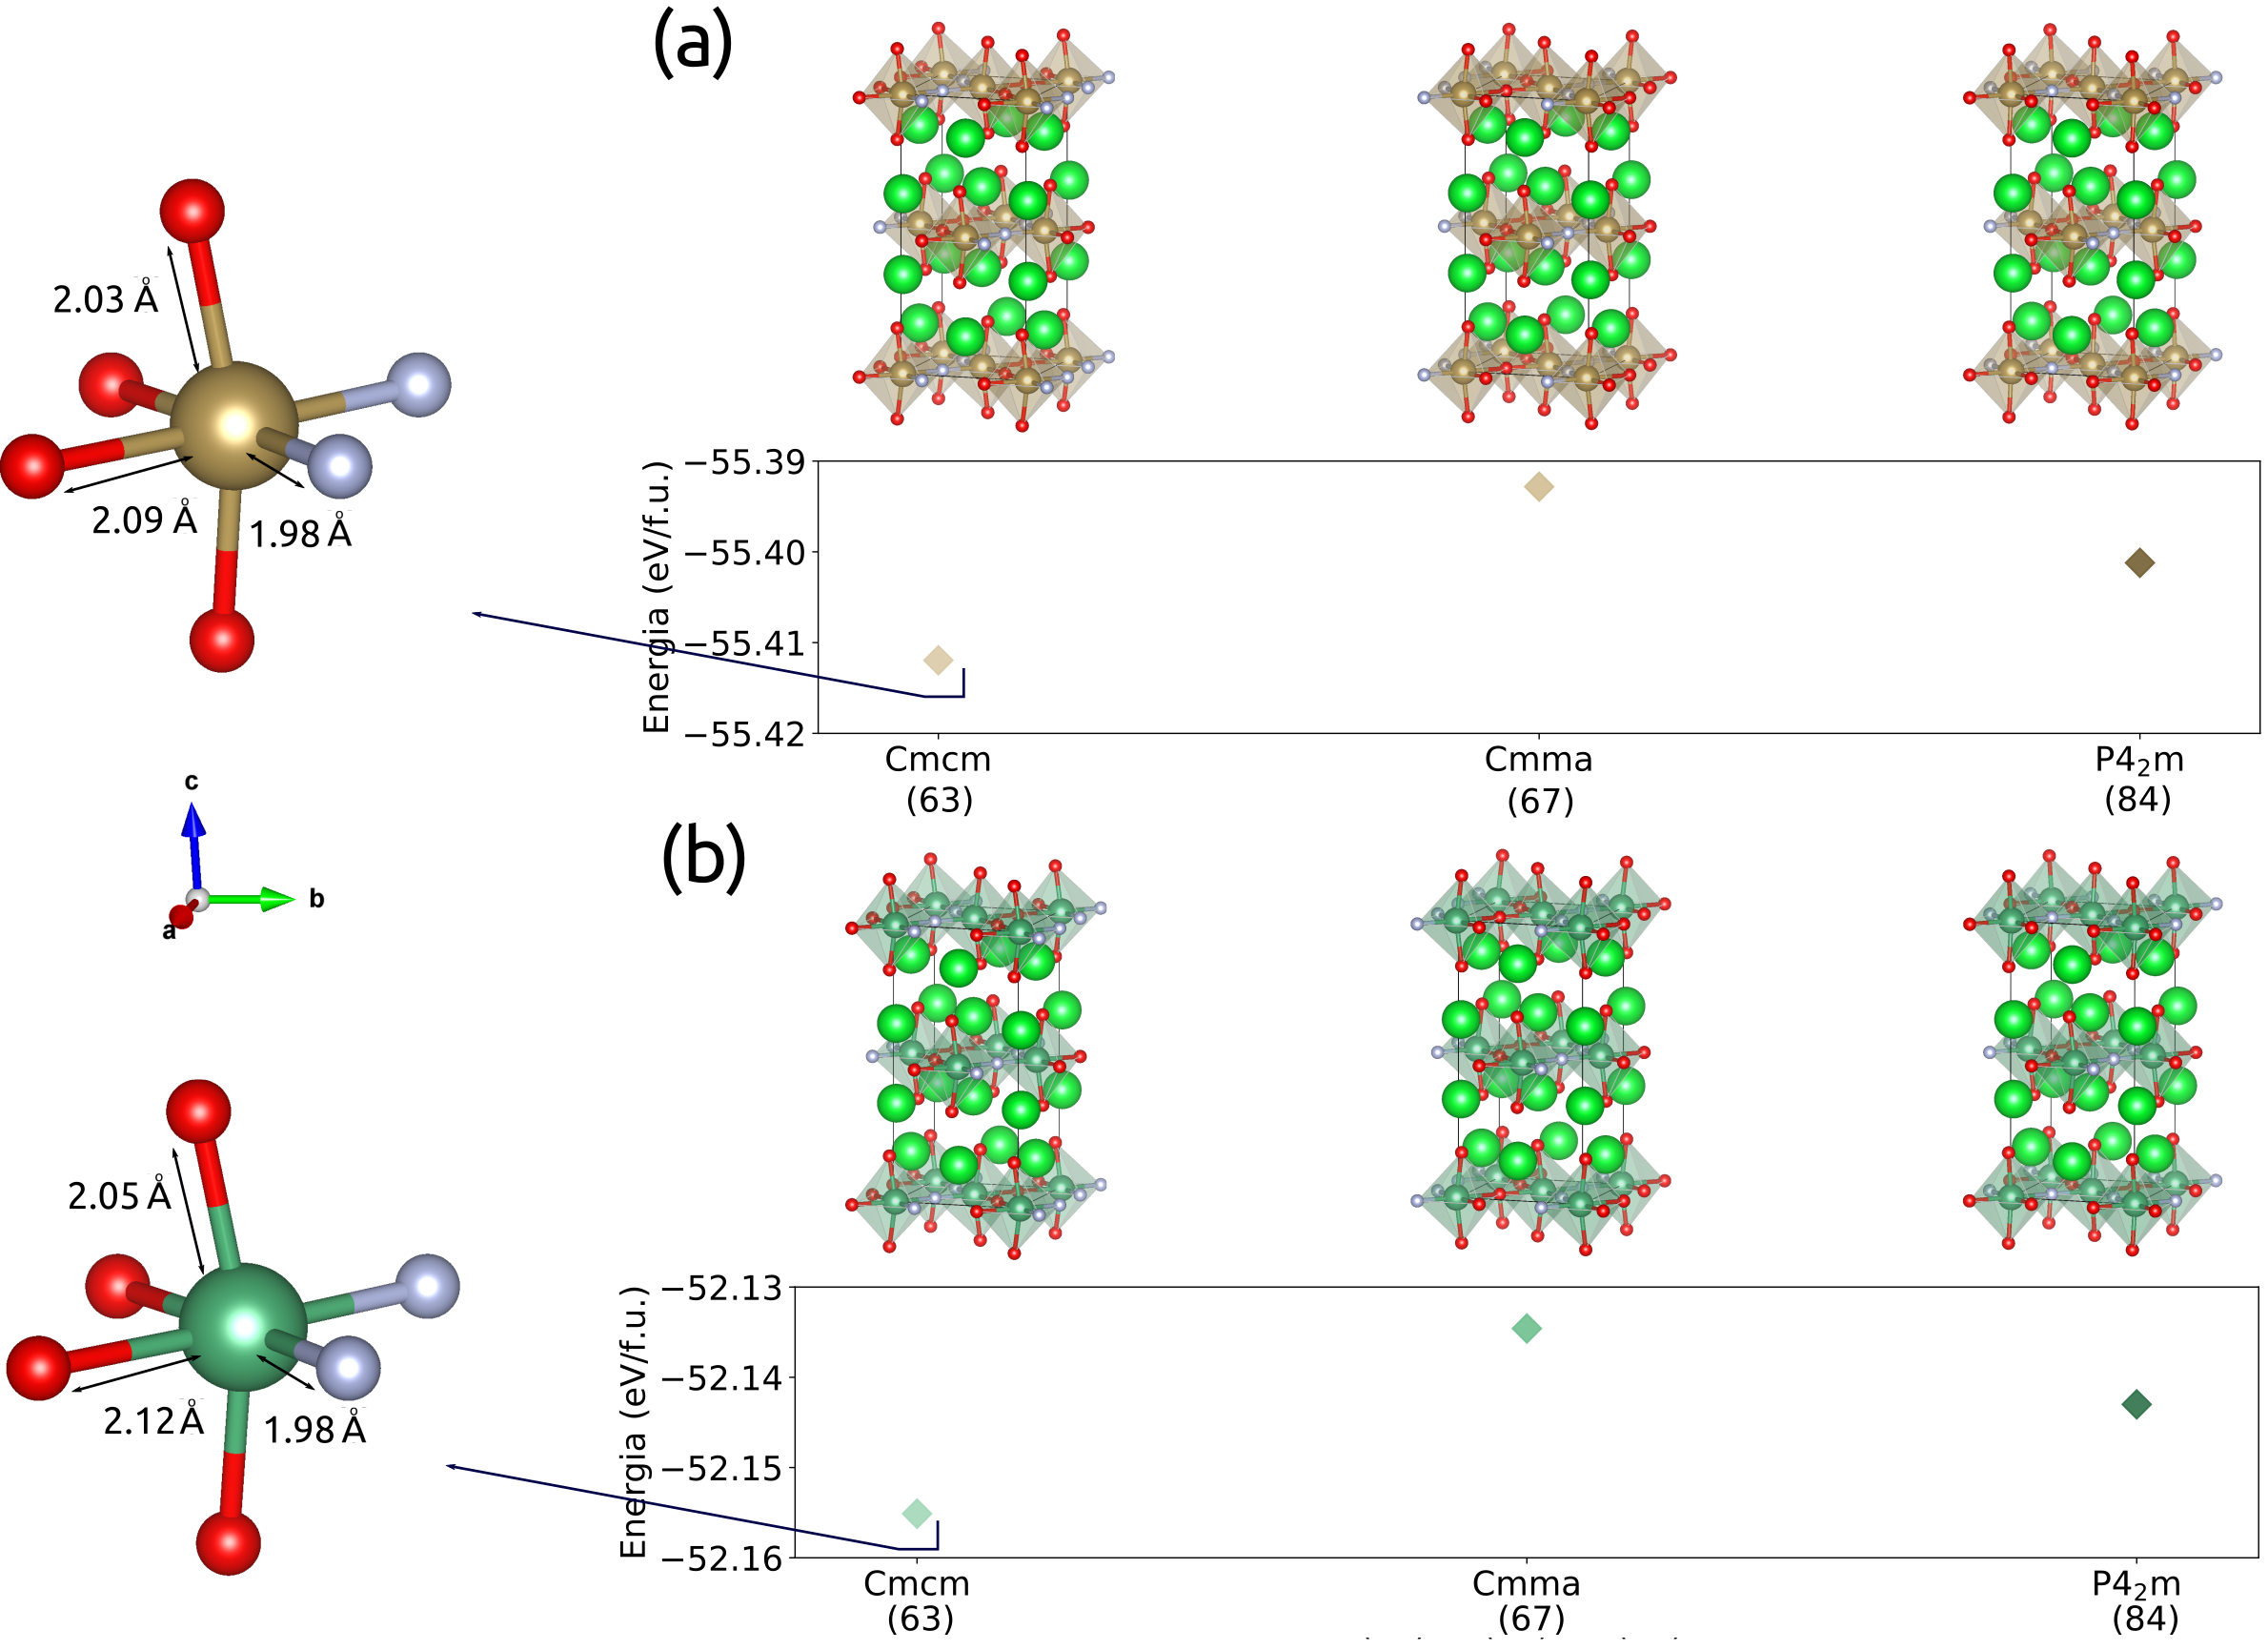
\includegraphics[width=\textwidth]{Figs/cis_energy_Ta.png}
    \caption{Energía estructural en relación a la simetría de grupo espacial de la configuración \textsc{rp}\emph{cis} (a) $Sr_{2}TaO_{3}N$ y (b) $Sr_{2}NbO_{3}N$.}
    \label{Fig. rp_cis}
\end{figure}

Las estructuras de mínima energía tienen simetría de grupo espacial $Cmcm(63)$ con un valor de $-55.41 eV$ y $-52.16 eV$ para $Sr_{2}TaO_{3}N$ y  $Sr_{2}NbO_{3}N$, respectivamente. Esta configuración favorable con ordenamiento aniónico \emph{cis} se sitúa sobre el plano y alterna capa a capa la orientación del ordenamiento, así como se reporta en la literatura \cite{Yang2011}.  Esta fase resulta ser la de mas baja energía para la concentración $x=1.0$, es decir, es mas estable que la configuración \emph{trans} con una diferencia de energía de $0.261 eV$ y $0.295  eV$ para $Sr_{2}TaO_{3}N$ y  $Sr_{2}NbO_{3}N$, respectivamente. Los parámetros de red de la configuración ($63$)-$Sr_{2}TaO_{3}N$ son $a=5.76750 \si{\angstrom}$, $b=5.84364 \si{\angstrom}$ y $c=12.44960 \si{\angstrom}$, $\alpha=\beta=\gamma=90^{\circ}$, y volumen $419.591059 \si{\angstrom}^{3}$,  lo parámetros de red de la configuración ($63$)-$Sr_{2}NbO_{3}N$ son $a=5.76750\si{\angstrom}$, $b=5.84364 \si{\angstrom}$ y $c=12.44960 \si{\angstrom}$, $\alpha=\beta=\gamma=90^{\circ}$, y volumen $419.591059  \si{\angstrom}^{3}$. Estos parámetro son de una supercelda creada para este ordenamiento aniónico. Comparando estos parámetro de red con las estructuras de óxidos puros, el parámetro en \emph{'a'} aumenta $\sim0.04  \si{\angstrom}$, siendo esta la dirección del enlace $(Ta,Nb)-N$, es decir la dirección del orden aniónico \emph{trans}, mientras que en la dirección \emph{'b'}, el parámetro de red disminuye $\sim0.01 \si{\angstrom}$.

La distancia de los enlaces $(Ta,Nb)-O$ en los sitios axiales se mantienen para ambos compuestos, entre $2.03  \si{\angstrom}$ y $2.05  \si{\angstrom}$, pero en los sitios ecuatoriales el enlace $(Ta,Nb)-O$ aumenta a $2,09  \si{\angstrom}$ y $2.12  \si{\angstrom}$ para $Sr_{2}TaO_{3}N$ y  $Sr_{2}NbO_{3}N$, respectivamente. Esto debido al desplazamiento sobre el plano del metal de transición $(Ta,Nb)$ en dirección [110] hacia el nitrógeno, ya que el enlace $(Ta,Nb)-N$ es de $1.98  \si{\angstrom}$ para ambos compuestos. El hecho de que el desplazamiento del metal de transición haya surgido, da un indicio de una posible fase ferroeléctrica en estas estructuras con ordenamiento aniónico \emph{cis}, ya que este fenómeno se da en materiales no centro-simétricos \cite{Cohen1992Oxides}.

%Las estructuras derivadas con orden de aniones \emph{trans} en el plano de aniones ecuatoriales son generalmente desfavorables porque tener aniones con dureza de Pearson similar uno al lado del otro maximiza la hibridación $\pi$ en los enlaces B-X. Por esta razón, la gran mayoría de oxifluoruros y oxinitruros exhiben unidades heterolépticas cis y fac, aunque estudios recientes han demostrado que la cepa puede inducir el orden de aniones trans \cite{Harada2019}. 





%Por lo tanto, para obtener una estructura polar que pueda exhibir ferroelectricidad o piroelectricidad, parecería esencial encontrar una ruta hacia una estructura trans ordenada. Una posible ruta para estabilizar un orden trans sería aprovechar la combinación de celosías epitaxiales en arquitecturas de película delgada para orientar los enlaces largos Ta-N perpendiculares al sustrato. \cite{Page2007LocalTheory}

%in dieléctrico SrT aO 2 N, el refinamiento de la estructura cristalina sugirió el orden de rango O / N y la inclinación local de octaedros cis-T aO 4 N 2,\cite{Masubuchi2013SynthesisCeramics}





%Esto es una consecuencia de la alta estabilidad del enlace metal-oxígeno que hace que la síntesis de compuestos de sustitución de aniones requiera el uso de métodos menos sencillos. \cite{Fuertes2012ChemistryPerovskites}









%La sustitución de O 2  por N 3  induce la sustitución cruzada de M 2+ por M 3+ o la formación de aniones vacantes, para mantener la neutralidad de carga [4] \cite{Masubuchi2013SynthesisCeramics}

%En la fase Ruddlesden-Popper, el átomo de niobio ($Nb$) muestra un estado de oxidación de $4+$ que no es estable en el aire a altas temperaturas, pero al sustituir un átomo de oxígeno por un átomo de nitrógeno en cada bloque de perovskita, pasaría de una oxidación de $Nb^{4+}$ a la más estable $Nb^{5+}$ como ocurre en la perovskita $SrNbO_{2}N$\cite{Tobias2004}. Además, debido a las similitudes en electronegatividad, polarizabilidad, radio iónico y número de coordinación entre el oxígeno y el nitrógeno, se permite la formación de estos tipos estructurales, así como la sustitución mutua de ambos aniones sobre los mismos sitios cristalográficos\cite{Tobias2004}.\\


 % Controladores PI y su conjunto estabilizante
% ------------------------------------------------------------------------
% ------------------------------------------------------------------------
% ------------------------------------------------------------------------
%                            Recomendaciones
% ------------------------------------------------------------------------
% ------------------------------------------------------------------------
% ------------------------------------------------------------------------

\chapter{ESTRUCTURA ELECTRÓNICA Y FONÓNICA DE LAS CONFIGURACIONES MAS ESTABLES}
% ------------------------------------------------------------------------
\section{ESTRUCTURA ELECTRÓNICA}

El inconveniente en usar \textsc{dft} es la descripción incorrecta de la estructura electrónica provocando el llamado "problema de bandagap", subestimando la correlación entre electrones, que a su vez impone dificultades para predecir interacciones intermoleculares precisas, energías de formación y estados de transición \cite{Tolba2018}. Para aumentar la precisión en los cálculos, es necesario introducir el esquema \textsc{dft+u} (Liechtenstein \cite{Lichtenstein1995StrongOrdering}), que es uno de los enfoques correctivos empleados para corregir el "problema de bandgap". Este parámetro se agrega al funcional de la densidad \textsc{gga+u}, corrigiendo la correlación de los electrones en los átomos tántalo y niobio a través de introducir un termino adicional en el hamiltoniano, agregado como una energía en los orbitales y corrige los orbitales y la separación entre ellos.

En esta sección, las estructuras electrónicas son calculadas mediante \textsc{dft} y \textsc{dft+u}, específicamente las configuraciones $Sr_{2}(Ta,Nb)O_{3}N$ \emph{trans} y \emph{cis} de mínima energía, siendo estas $Immm(71)$ y $Cmcm(63)$, respectivamente. Además, se realiza un análisis de la brecha entre la banda de valencia y la banda de conducción, la contribución orbital y una posible aplicación: fotocatálisis para división de agua.  

\section{Relevantes detalles computacionales: Cálculo auto-consistente}

El cálculo auto-consistente es un método iterativo para resolver el problema de valores propios $\epsilon_{i}$ y funciones propias $\Psi_{i}(\vec{r})$ de las ecuaciones de Khon-Sham (ecuación \ref{Eq. KS}) bajo la teoría funcional de la densidad. El problema es que $V_{\text{ext}}$ y $V_{xc}$ dependen de la densidad $n$, y esta a su vez depende de las funciones propias  $\Psi_{i}(\vec{r})$ desconocidas, lo que implica que debe ser determinada de forma auto-consistente.  Para resolver la ecuación de Schrodinger se debe estimar una densidad electrónica inicial $n^{j}(\vec{r})$ agregando las densidades electrónicas de los átomos aislados teniendo en cuenta los sitios atómicos de la estructura. Usando esta densidad obtenemos un primer potencial $V_{\text{Hartree}}+V_{xc}$ que es agregado al potencial de Khom-Sham (ecuación \ref{Eq. V_ks}), y se resuelve el hamiltoniano de Khom-Sham (ecuación \ref{Eq. KS}) discretizando el espacio en punto $k$ para encontrar los valores propios y las funciones propias \cite{lin_lu_ying_2019}. Con estos orbitales encontrados se construye una nueva densidad electrónica $n^{\text{j+1}}(\vec{r})$ y se repite el proceso de forma iterativa hasta que la densidad inicial $n^{j}(\vec{r})$ y la densidad final $n^{\text{j+1}}(\vec{r})$ sean iguales \cite{Woods2018Theory}, es decir, cuando se encuentra el estado base de la densidad electrónica que minimiza el hamiltoniano Khon-Sham \cite{GiustinoFeliciano2014Mmud}.

%Los resultados de los cálculos presentados fueron obtenidos usando la plataforma \texttt{GridUIS-2}, desarrollada por el Centro de Supercomputación y Cálculo Científico de la Universidad Industrial de Santander (\textsc{sc3uis}). Esta acción es soportada por la Vicerrectoría de Investigación y Extensión de la \textsc{uis} (\textsc{vie-uis}) y diferentes grupos de investigación de la universidad. (\url{http://www.sc3.uis.edu.co})

\subsection{Configuración $Sr_{2}(Ta,Nb)O_{3.5}N_{0.5}$  $Pmmm(47)$}

En este caso, la concentración x=0.5 hay pocos reportes en la literatura, así que se determinó si el parámetro \textsc{u} corrigió los orbitales de manera considerable mediante un análisis de estructura de bandas. Se realizó un calculo de bandas para la fase Ruddlesden-Popper $Sr_{2}BO_{3.5}N_{0.5}(B=Ta/Nb)-Pmmm$, que es la estructura de mínima energía. Los resultados son los siguientes:

\begin{figure}[H]
    \centering
    \includegraphics[width=0.4\textwidth]{Figs/bandas-con-u_ta35.eps}
    \includegraphics[width=0.4\textwidth]{Figs/bandas-con-u_nb35.eps}
    \caption{Estructura de bandas electrónicas de la fase Ruddlesden-Popper ($Sr_{2}(Ta,Nb)O_{3}N$).}
    \label{Fig. bandas_35}
\end{figure}

Específicamente en la gráfica \ref{Fig. bandas_35}(b), se observa que en el punto $\Gamma$ se superponen las bandas de conducción $d$ del niobio con las bandas de valencia $p$ del nitrógeno, lo que indican malos resultados computacionalmente. Para ambas gráficas en \ref{Fig. bandas_35}, el supuesto nivel de Fermi que se obtuvo esta en $-1.8  eV$, lo cual es incorrecto, el nivel de Fermi debe estar idealmente en $0 eV$, lo que confirma que el parámetro \textsc{u} falló en corregir los orbitales atómicos. La energía \textsc{u} no corrige adecuadamente los orbitales atómicos de la fase Ruddlesden-Popper $Sr_{2}AO_{3.5}N_{0.5}(B=Ta/Nb)$ debido a la presencia de poco nitrógeno en los octaedros. Se debe realizar un estudio acerca del valor del parámetro \textsc{u} para esta fase, en caso de que la corrección falle se podría recurrir a otras teorías como 'dynamical mean-field theory' \textsc{dmft} combinada con \textsc{dft}.

\subsection{Configuración $Sr_{2}(Ta,Nb)O_{3}N$ \emph{trans} $Immm(71)$}

Los puntos de alta simetría que guían el camino en la zona de Brillouin de la estructura electrónica se obtuvieron mediante el código \textsc{vaspkit} \cite{Wang2019VASPKITCode}:

$$\Gamma-X-F_{2}/\Sigma_{0}-\Gamma-Y_{0}/U_{0}-X/\Gamma-R-W-S-\Gamma-T-W$$

\begin{figure}[H]
    \centering
    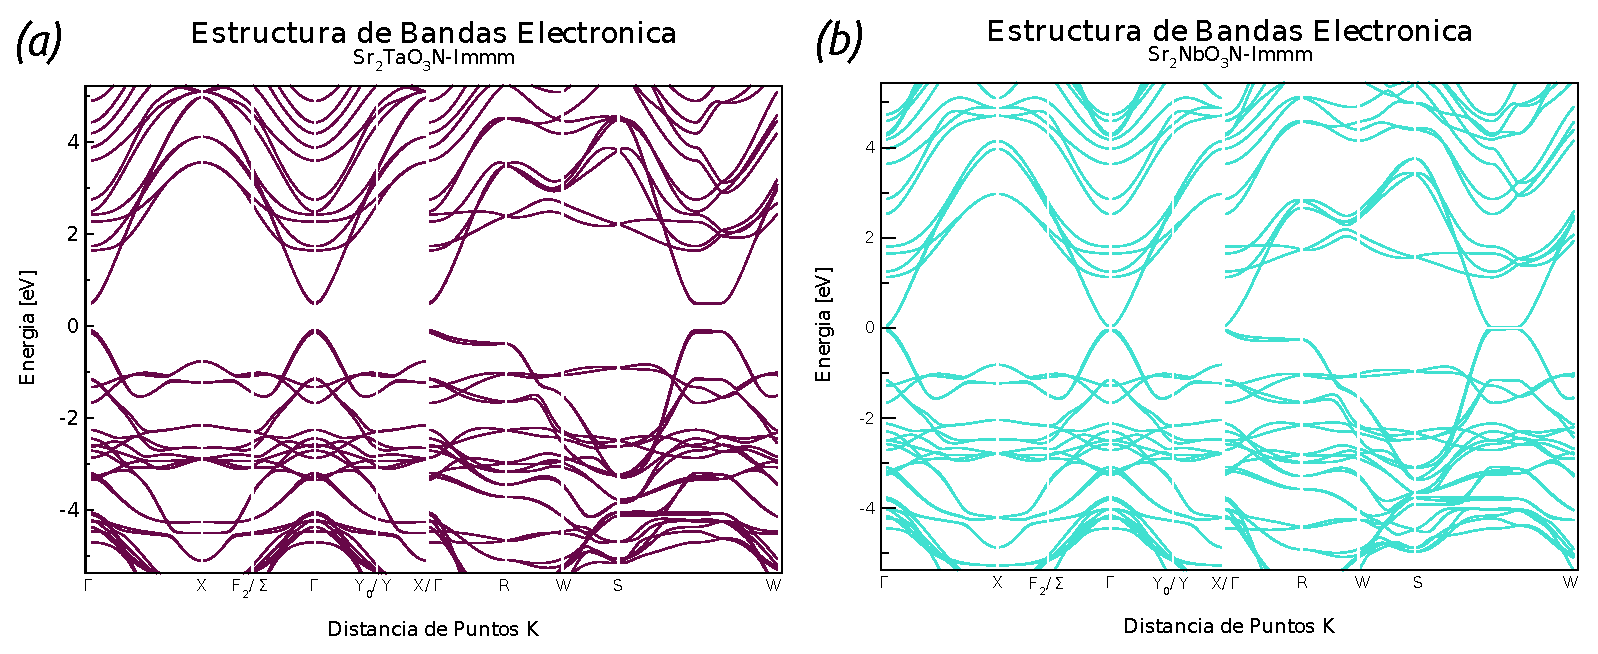
\includegraphics[width=\textwidth]{Figs/bands-trans_sin-U.eps}
    \caption{Estructura de bandas electrónicas de la configuración con ordenamiento aniónico \emph{trans}  (a) $Sr_{2}TaO_{3}N$ y (b) $Sr_{2}NbO_{3}N$, sin tener en cuenta el parámetro \textsc{u}.}
    \label{Fig. bandas_trans-sin-u}
\end{figure}

Al observar principalmente las bandas de conducción y las de valencia en la figura \ref{Fig. bandas_trans-sin-u}(a), la configuración \textsc{rp}$Sr_{2}TaO_{3}N$  muestra un brecha en el punto $\Gamma$ de $0.5728 eV$, lo que indica que el material es aislante. Analizando la figura \ref{Fig. bandas_trans-sin-u}(b) la configuración \textsc{rp}$Sr_{2}NbO_{3}N$ muestra una brecha insignificante de $0.0001 eV$, mostrando un comportamiento conductor, lo cual no van en concordancia con los datos reportados en la literatura \cite{Diot1999CrystalN,Bouri2018}. Por ende, se hace necesario agregar el parámetro \textsc{u} a los cálculos en \textsc{dft}. Dentro del cálculo se tuvo en cuenta el parámetro de corrección \textsc{u} con un valor de $4.0  eV$, los resultados son los siguientes:

\begin{figure}[H]
    \centering
    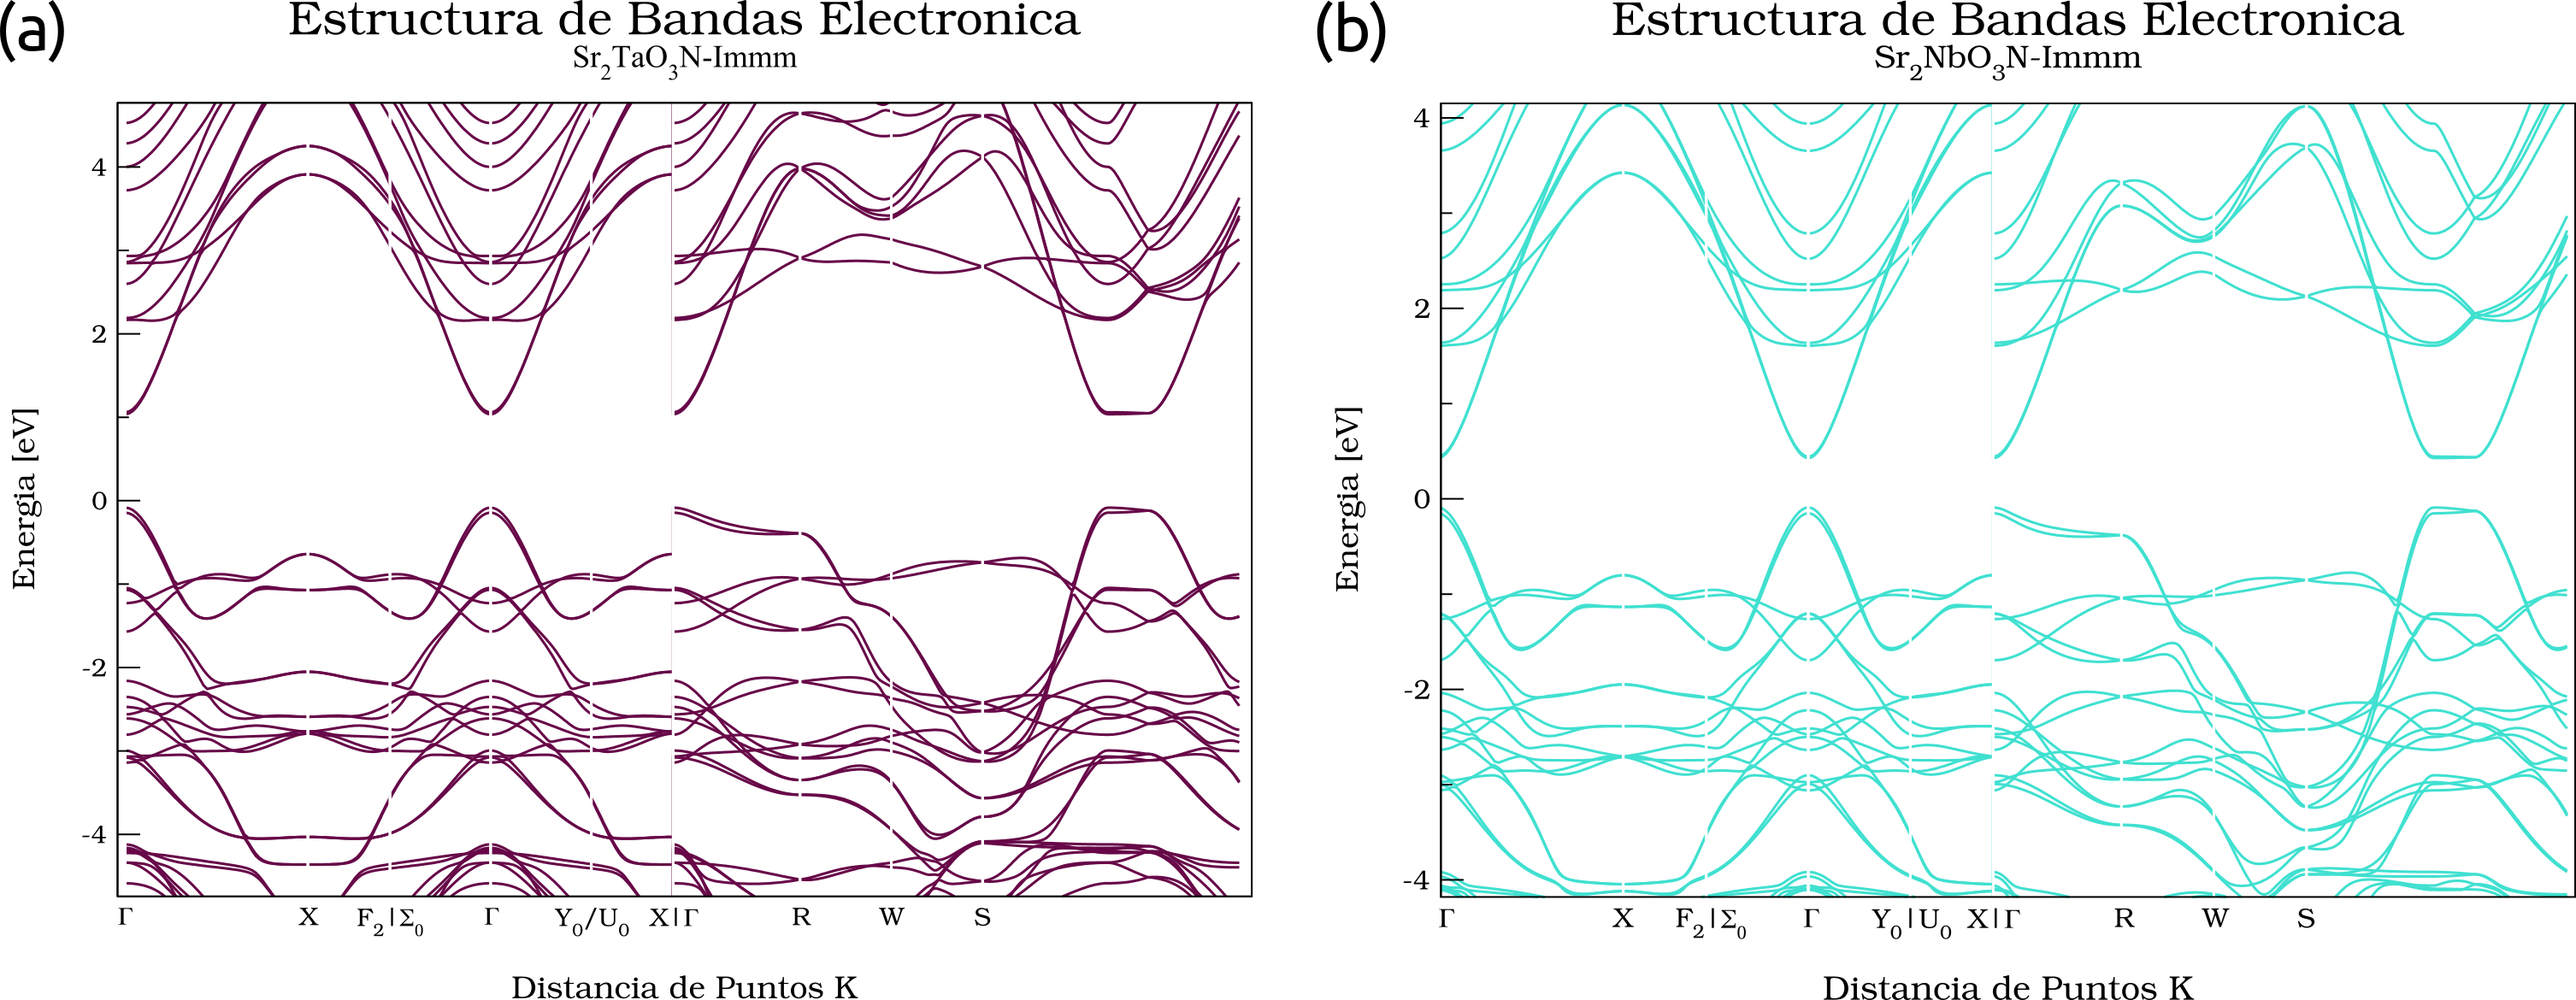
\includegraphics[width=\textwidth]{Figs/bands-con-u_trans.png}
    \caption{Estructura de bandas electrónica de la configuración con ordenamiento aniónico \emph{trans}  (a) $Sr_{2}TaO_{3}N$ y (b) $Sr_{2}NbO_{3}N$, calculadas mediante \textsc{dft+u} con valor de $U=4.0  eV$}
    \label{Fig. bands-con-u_trans}
\end{figure}

En el caso de las bandas electrónicas de $Sr_{2}TaO_{3}N-Immm$ (figura \ref{Fig. bands-con-u_trans}(a)), el bandgap en el punto $\Gamma$ aumenta a un valor de $1.1202  eV$ comparado con las bandas previas sin el parámetro \textsc{u} donde se obtenía un valor de $0.5728  eV$. Las bandas $d$ del niobio y del tántalo tienen forma parabólica en el punto $\Gamma$, lo que indican buenos resultados. En el caso de las bandas electrónicas de $Sr_{2}NbO_{3}N-Immm$ (figura \ref{Fig. bands-con-u_trans}(b)), el bandgap en el punto $\Gamma$ aumenta a un valor de $0.5194  eV$ comparado con las bandas previas sin el parámetro \textsc{u} donde se obtenía un valor casi nulo. En ambos casos, se evidencia una apertura de la brecha entre la banda de valencia y la banda de conducción, esto debido al parámetro\textsc{u} agregado en los metales de transición.

Para un mayor análisis, se define un camino estándar en la zona de Brillouin para las configuraciones $Sr_{2}(Ta,Nb)O_{3}N$ \emph{trans-}$Immm$ y \emph{cis-}$Cmcm$, con el fin de comparar y especificar los cambios que surgen en las la estructura electrónica. El camino en el espacio $k$ es:

$$(0,0,0)-(0.5,0,0)-(0.5,0.5,0)-(0,0,0)-(0.5,0.5,0.5)-(0,0,0.5)$$

Además, se realiza la proyección atómica de las bandas electrónicas,  es decir, las bandas de los átomos de estroncio, niobio, tántalo, oxigeno y nitrógeno están marcadas con el color indicado en cada elemento atómico de la siguiente fórmula:

$$\textcolor{purple}{Sr_{2}}(\textcolor{orange}{Ta},\textcolor{green}{Nb})\textcolor{O}{O_{3}}\textcolor{blue}{N}$$

\begin{figure}[H]
    \centering
    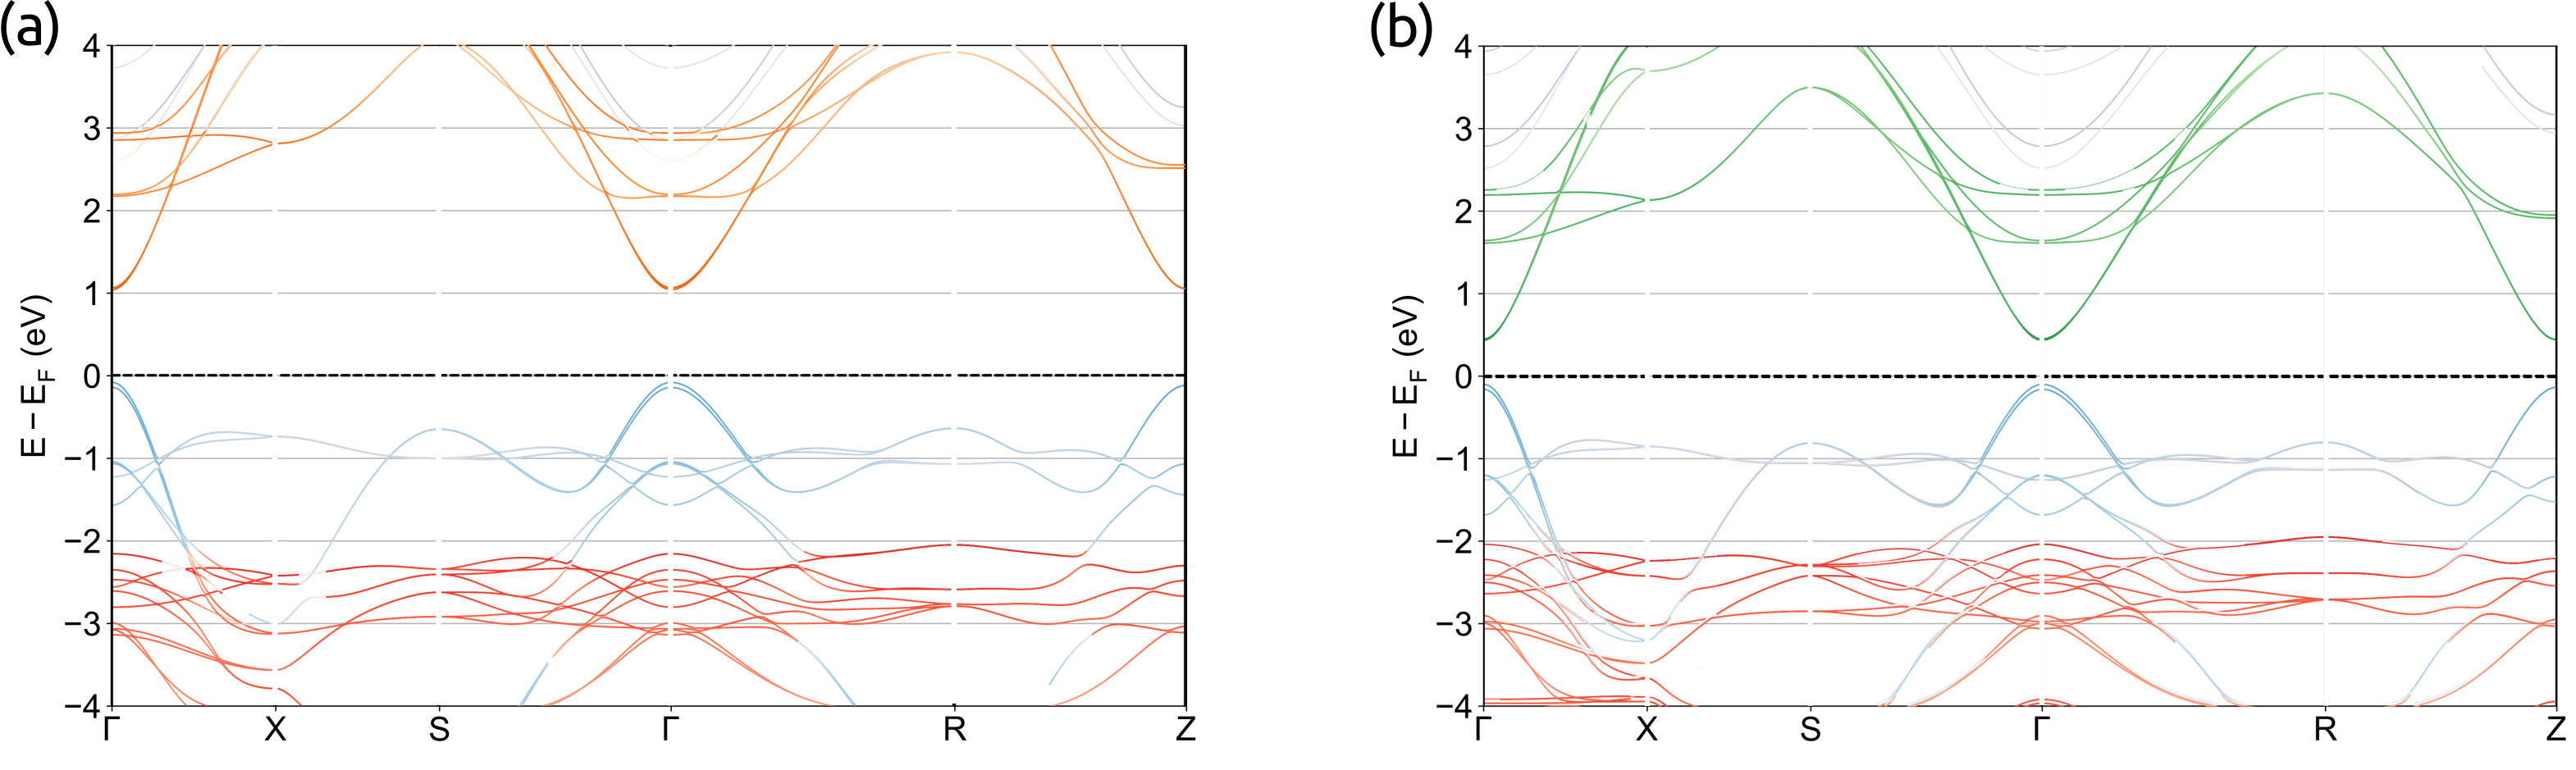
\includegraphics[width=1\textwidth]{Figs/trans-all.png}
    \caption{Estructura de bandas electrónicas de la configuración con ordenamiento aniónico \emph{trans} (a)$Sr_{2}TaO_{3}N$ y  (b)$Sr_{2}NbO_{3}N$.}% (c-d) Contribución orbital $d_{xy}$ del metal de transición $(Ta,Nb)$.}
    \label{Fig. bandas_trans_estandar}
\end{figure}

Las bandas de los metales de transición $(Ta, Nb)$ están cerca a Fermi, se posicionan como bandas de conducción, por lo que al agregar el parámetro \textsc{u}$=4.0  eV$ aumentan en energía, observando la subida de las bandas en la estructura electrónica de la figura \ref{Fig. bandas_trans_estandar} respecto al cálculo sin el parámetro \textsc{u}, y por ende un ensanchamiento del bandgap directo en el punto $\Gamma$. Esto evidencia el papel que juega el parámetro \textsc{u} en el comportamiento de los metales de transición ($Ta,Nb$). En cuanto a la banda de valencia, los átomos de nitrógeno ocupan lo estados cercano a Fermi, reduciendo el bandgap respecto a los óxidos puros \cite{Diot1999CrystalN,Tang2020light,Cen2019OptimizedSplitting}, esto debido a que el nitrógeno ($N^{3-}$)  tiene menos electronegatividad que el oxígeno ($O^{2-}$) y los orbitales $N-2p$ se encuentran por encima de los orbitales $O-2p$ \cite{Cen2019OptimizedSplitting}. También se puede observar en el hecho de que el oxigeno tiene menos espacio en su orbital para recibir electrones, en cambio el nitrógeno tiene un espacio extra para recibir electrones, por lo que el orbital del nitrógeno sube en energía. Por otro lado, el estroncio inicia apareciendo en $E-E_{f}=3 eV$ y más altas energías, por lo que no aporta a las bandas de conducción. Esto debido a la electronegatividad del estroncio $Sr:0.95$ en comparación con el metal de transición $(Ta,Nb):(1.5,1.6)$, así que el metal de transición se sitúa en las bandas de conducción, pero el estroncio no lo hace. El bandgap de $Sr_{2}TaO_{3}N$ es de $1.1202  eV$, lo que hace a este material mas favorable en el uso de fotocatálisis para división de agua, en comparación con el bandgap de $Sr_{2}NbO_{3}N$ de $0.5194 eV$. Lo reportado en la literatura, como en \cite{Cen2019OptimizedSplitting} con un bandgap de $2.12 eV$, en \cite{Clarke2002} es de $1,97 eV$ y en \cite{Bouri2018} es de $2.0 eV$, muestran bandgaps muy amplios respecto a nuestros resultados. Al parámetro \textsc{u}, el bandgap se abrirá, por lo que se sugiere aumentarlo para este ordenamiento \emph{trans}.

%La contribución orbital en el metal de transición es de $(Ta,Nb)-d_{xy}$ en el punto $\Gamma$ de la estructura electrónica, lo que indica un enlace $\pi$ con el orbital del nitrógeno $N-p_{x}$.

\subsection{Configuración $Sr_{2}(Ta,Nb)O_{3}N$ \emph{cis} $Cmcm(63)$}

El camino estándar en la zona de Brillouin para las configuraciones $Sr_{2}(Ta,Nb)O_{3}N$ \emph{cis-}$Cmcm$ es:

$$(0,0,0)-(0.5,0,0)-(0.5,0.5,0)-(0,0,0)-(0.5,0.5,0.5)-(0,0,0.5)$$

$$\textcolor{purple}{Sr_{2}}(\textcolor{orange}{Ta},\textcolor{green}{Nb})\textcolor{O}{O_{3}}\textcolor{blue}{N}$$

\begin{figure}[H]
    \centering
    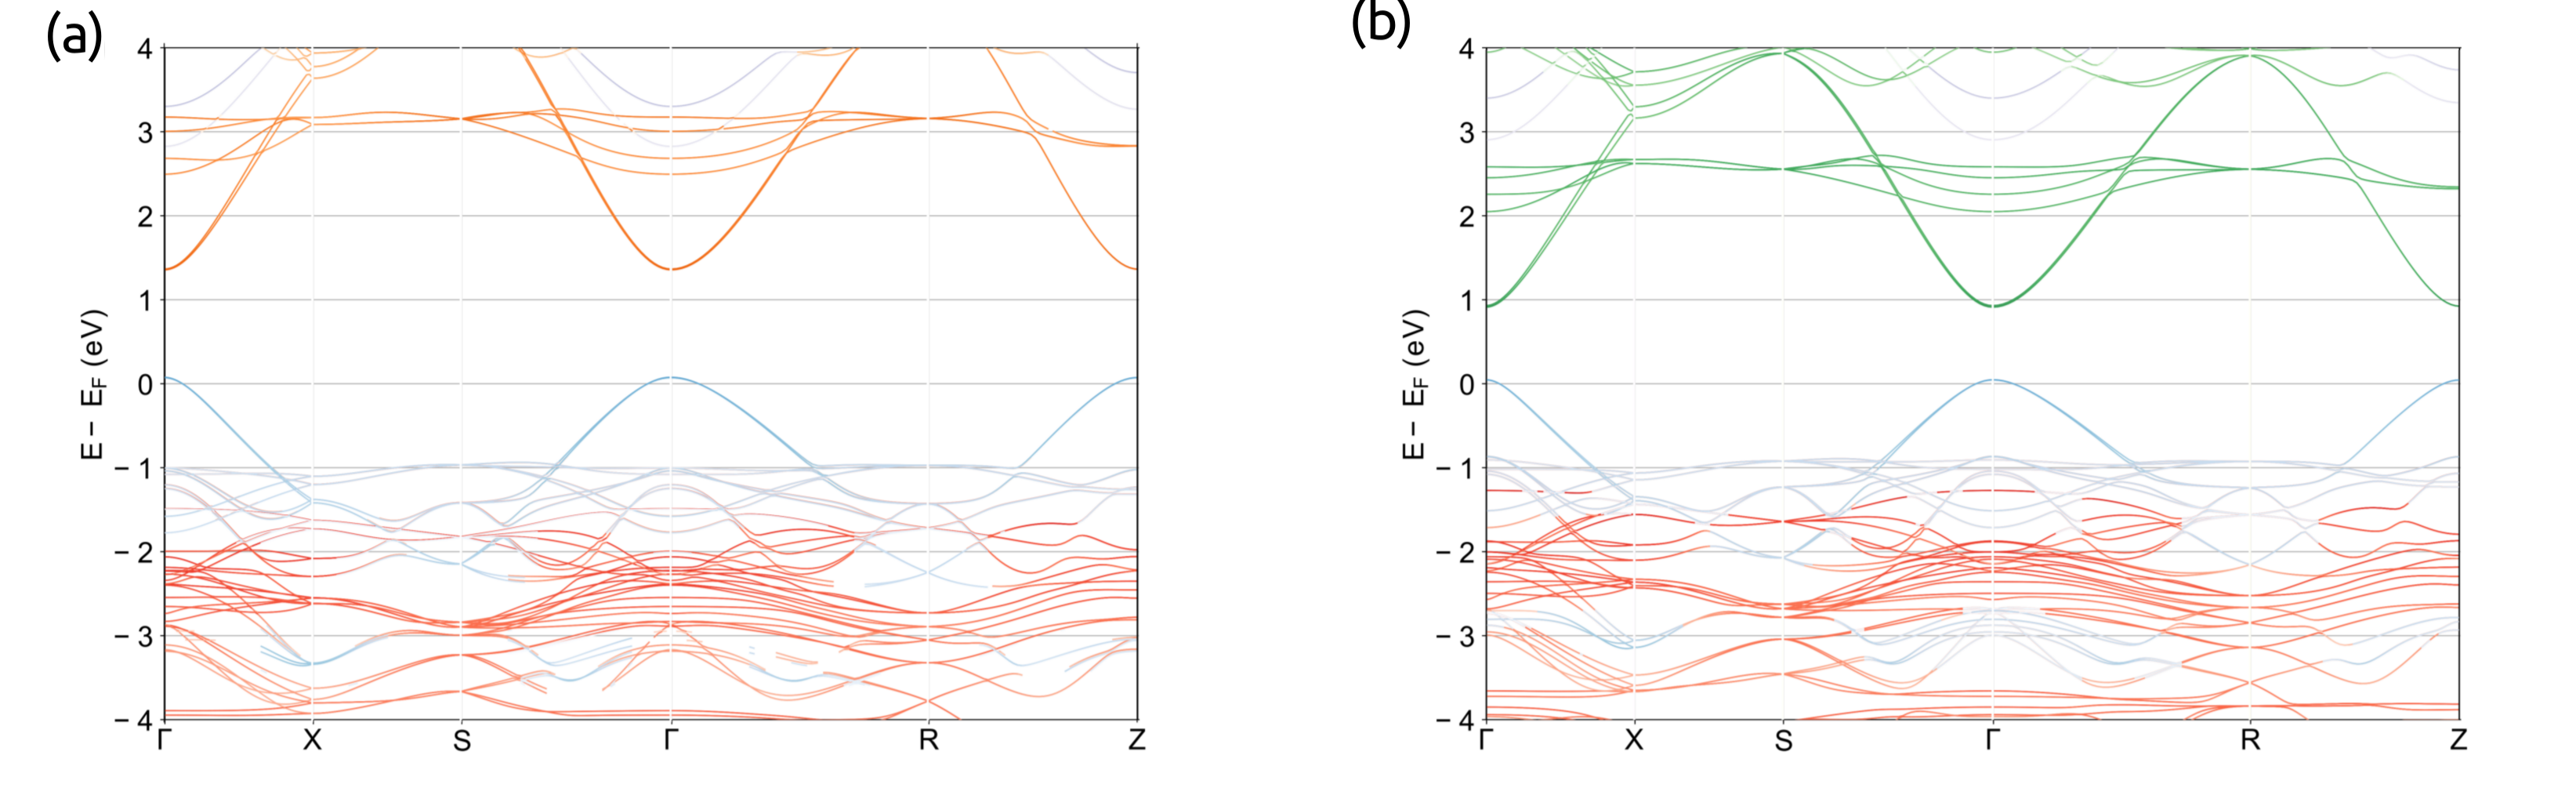
\includegraphics[width=1\textwidth]{Figs/cis_all.png}
    \caption{Estructura de bandas electrónicas de la configuración con ordenamiento aniónico \emph{cis} (a)$Sr_{2}TaO_{3}N$ y  (b)$Sr_{2}NbO_{3}N$.}
    \label{Fig. bandas_cis_estandar}
\end{figure}

Similar a lo que sucede en la configuración \emph{trans}, las bandas de los metales de transición $(Ta, Nb)$ se posicionan como bandas de conducción. Los átomos de nitrógeno ocupan la banda de valencia, reduciendo el bandgap respecto a los óxidos puros. El bandgap de $Sr_{2}TaO_{3}N$ es de $1.2916  eV$, es un oxinitruro relevante por su aplicación como un muy eficiente fotocatalizador para la oxidación de agua en $O_{2}$ \cite{Tobias2004}, en comparación con el bandgap de $Sr_{2}NbO_{3}N$ $0.8636  eV$, además de un mejor ancho de banda comparado con el orden de aniones \emph{trans}. En el caso de \emph{cis-}$Sr_{2}TaO_{3}N$,. Lo reportado en la literatura para el orden de aniones \emph{cis-}$Sr_{2}TaO_{3}N$ es de $1.128 eV$ \cite{Bouri2018}, obteniendo resultados coherentes con la literatura.% La contribución orbital en el metal de transición es de $(Ta,Nb)-d_{x^{2}-y^{2}}$ en el punto $\Gamma$ de la estructura electrónica. La diferencia con la configuración \emph{trans} es que la contribución de los orbitales en el nitrógeno es parcial entre $N-p_{x}$ y $N-p_{y}$, por lo que los orbitales se hibridizan formando un enlace $\pi$.

El ordenamiento aniónico \emph{cis} sobre el plano es preferida por los nitrógenos, y puede explicarse en términos de la utilización máxima de los orbitales $d$ vacantes en el enlace $\pi$ con los pares de aniones solitarios. En la configuración \emph{cis}, los cuatro pares solitarios de aniones de tipo $p$ pueden interactuar con tres orbitales $d$ vacantes del metal de transición, mientras que en el ordenamiento \emph{trans} interactúan con dos orbitales $d$ \cite{Fuertes2012ChemistryPerovskites}, el lado opuesto donde se posiciona el nitrógeno hay un oxígeno, lo que favorece el desplazamiento del catión hacia el anión menos electronegativo para facilitar la hibridación orbital \cite{Harada2019PredictingOrder}. Como consecuencia, se maximiza la covalencia $(Ta-Nb)(d\pi)-N(p\pi)$ favoreciendo el ordenamiento \emph{cis} sobre la \emph{trans}\cite{Yang2011,Ebbinghaus2004PowderK}. El hecho de que el nitrógeno sea menos electronegativo que el oxígeno conduce a más enlaces covalentes en los nitruros y oxinitruros que en los óxidos. Las sustituciones de nitrógeno por oxígeno modificaron la estructura de bandas, reduciendo la brecha en comparación con los óxidos puros \cite{Diot1999CrystalN}. 






%La estructura en capas conduce a un enlace debilitado de los orbitales T a t 2g con un componente z (es decir, d xz y d yz), que se vuelven menos dispersivos y aparecen como el pico marcado por encima de 2  eV en el dos. Debido al orden N completo en el plano, la banda d xy debería ser más dispersiva y extenderse a energías más bajas que en una perovskita no estratificada comparable (es decir, $Sr_{2}TaO_{2}N$). \cite{Bouri2018}
%Goodnough y Longo [29] señalan que cuando el catión A disminuye de tamaño, lo que lleva a un canto cooperativo de los octaedros entre sí, el acortamiento de la distancia A  O mejora la unión $\sigma$ entre los cationes A y los O (2p) orbitales, que interactúan en un sentido $\pi$ con los orbitales M (d). Esto tiene el efecto de estabilizar los orbitales O (2p), reduciendo la mezcla de homo-lumo en los octaedros y apagando así la distorsión ferroeléctrica de los octaedros. \cite{Clarke2002OxynitridePerovskites}



%La Ruddlesden-Popper es como una perovskita que se desvía porque hace que halla mas contenido de unos átomos que en otros. Se tienen los octaedros pero se arman por capas, estas capas se dislocan, en este caso abajo hay un metal de transición y arriba no hay nada, entonces la carga se confina diferente respecto a la perovskita. Se usan para baterías, fotocatálisis, almacenamiento de nitrógeno, con luz hace water splitting. En las baterías de hidrógeno, cuando la estructura es polar, puede separar mas el agua, es decir baterías de hidrógeno a través de separar el agua.\\


% ------------------------------------------------------------------------  % Recomendaciones
% ------------------------------------------------------------------------
% ------------------------------------------------------------------------
% ------------------------------------------------------------------------
%                            Trabajo futuro
% ------------------------------------------------------------------------
% ------------------------------------------------------------------------
% ------------------------------------------------------------------------
%\chapter{DISPERSIÓN DE FONONES}

\section{ESTRUCTURA FONÓNICA}

Con el desarrollo de nuevos dispositivos electrónicos se hace indispensable el conocimiento de posibles fases ferroeléctrias para memorias informáticas y dispositivos móviles, incluyendo computación en la nube \cite{Scott2007Ferroelectrics}, ya que la respuesta de la polarización espontánea a excitaciones externas genera efectos físicos como piezoelectricidad, piroelectricidad y propiedades dieléctricas \cite{Shi2016SymmetryFerroelectrics}. En esta sección se discute la dispersión de fonones de las estructuras $Sr_{2}(Ta,Nb)O_{3}N$ para dos ordenamientos aniónicos: \emph{trans-}$Immm(71)$ y \emph{cis-}$Cmcm(63)$ y las fases estables y meta-estables encontradas para estos dos ordenamientos.

\subsection{Relevantes detalles computacionales: Cálculo de estructura fonónica}

El cálculo de estructura fonónica, ó también llamada dispersión de fonones es aplicado ampliamente en materia condensada para el análisis de posibles acoplamientos electrón-fonón ó espín-fonón, y transiciones de fase debido a inestabilidades en la estructura. Lo primero es crear una supercelda de la estructura a investigar, en el presente trabajo se realiza una supercelda $2\times2\times1$ para $Sr_{2}(Ta,Nb)O_{3}N$ \emph{cis-}$Cmcm(63)$ y \emph{trans-}$Immm(71)$. La supercelda no tuvo cambios en dirección [001] debido a la simetría por capas de la estructura, no lo requería. Con la supercelda se procede a hacer el cálculo para encontrar la matriz dinámica, que contiene las constantes de fuerza ínter-atómica, definidas como la segunda derivada de la energía respecto a los desplazamientos atómicos. La imposibilidad de converger este cálculo computacionalmente pesado, con 56 átomos para el orden \emph{trans}, y 112 átomo para el orden \emph{cis}, se establece el método de diferencias finitas donde se desplaza un átomo en una dirección especifica y se calcula cómo responden los átomos vecinos al desplazamiento de fuerzas. Los desplazamientos fueron encontrados mediante el código \textsc{phonopy} \cite{Togo2015phonopy}. Para el ordenamiento aniónico \emph{trans} se obtuvieron 7 desplazamientos, mientras que para el orden de aniones \emph{cis} se obtuvieron 14 desplazamientos, los cuales fueron unidos para generar la matriz constantes de fuerzas interatómicas. Una vez se genera la matriz, se agrega a la celda unitaria, mostrando las curva de dispersión de fonones. Cabe aclarar que en \textsc{phonopy}, las simetrías se buscan con las operaciones de simetría del grupo espacial de la estructura cristalina y comprobando si es invariante después de las operaciones de simetría. En este análisis, se utiliza una tolerancia de distancia $1\times10^{-3}$e en la configuración \emph{cis} para tolerar las pequeña desviaciones de la celda, y el valor predeterminado es $1\times10^{-5}$, el cual fue usado en la configuración \emph{trans}. 

Se agregó una corrección no analítica usando el método Wang \textit{et. al.} \cite{Wang_2010-nac} que usa las constantes de fuerza calculadas en el espacio real y las interacciones dipolo-dipolo calculadas por la teoría de respuesta lineal en el espacio recíproco. La corrección se aplica a la matriz dinámica y se activa con el archivo \textsc{born}, el cual contiene la información de la carga efectiva de Born y la constante dieléctrica \cite{Pick1970Aproximation}. En los cristales polares, surgen campos eléctricos macroscópicos de largo alcance que están asociados con fonones ópticos longitudinales de onda larga. Estos campos eléctricos son el resultado del carácter de largo alcance de la interacción de Coulomb \cite{Baroni2001theory}, y son responsables del conocido fenómeno de división \textsc{lo-to}, es decir, el cambio de frecuencia entre fonones ópticos longitudinales y ópticos transversales en el centro de la zona de Brillouin. Este acoplamiento entre fonones ópticos y campos eléctricos se cuantifica mediante la carga efectiva de Born, que se define mediante:

\begin{equation}
    Z^{\circ}_{\kappa\alpha\beta}=-\frac{\delta^{2}\Vec{E}}{\delta\epsilon_{\beta}\delta\\Vec{u}_{\kappa\alpha}}
    \label{Eq. Born}
\end{equation}

Son el coeficiente de proporcionalidad que relaciona un cambio en la dirección $\alpha$ debido a un campo eléctrico homogéneo aplicado en dirección $\beta$.

\subsection{Configuración con ordenamiento tipo \emph{trans}}

Se presenta la curva de dispersión de fonones de las configuraciones \emph{trans-}$Immm(71)$ de las estructuras $Sr_{2}TaO_{3}N$ y $Sr_{2}NbO_{3}N$ ilustradas en la figura \ref{trans-phon}(a) y \ref{trans-phon}(b), respectivamente.

Para el caso de la configuración \emph{trans-}$Sr_{2}TaO_{3}N$ (figura \ref{trans-phon}(a)), la dispersión de fonones muestra un modo imaginario en el punto $X(0.0,0.5,0.0)$ con frecuencia de $-26.43cm^{-1}$, un modo imaginario en el punto $M(0.5,0.5,0.0)$ con frecuencia de $-97.46cm^{-1}$, y 2 modos imaginarios en el punto $R(0.5,0.5,0.5)$ con frecuencias de $-84.87cm^{-1}$ y $-49.21cm^{-1}$. Para el caso de la configuración \emph{trans-}$Sr_{2}NbO_{3}N$ (figura \ref{trans-phon}(b)) se observan 10 modos imaginarios en la zona de Brillouin: 4 en el punto $\Gamma(0.0,0.0,0.0)$ con frecuencias de $-129.06cm^{-1}$, $-114.48cm^{-1}$, $-92.34cm^{-1}$ y $-91.77cm^{-1}$; y 2 modos imaginarios en cada punto $X(0.0,0.5,0.0)$ con frecuencias de $-56.1016cm^{-1}$ y $-45.29cm^{-1}$; $M(0.5,0.5,0.0)$ con frecuencias de $-110.20cm^{-1}$ y $-44.43cm^{-1}$; y $R(0.5,0.5,0.5)$ con frecuencias de $-97.91cm^{-1}$ y $-70.75cm^{-1}$.

\begin{figure}[h!]
    \centering
    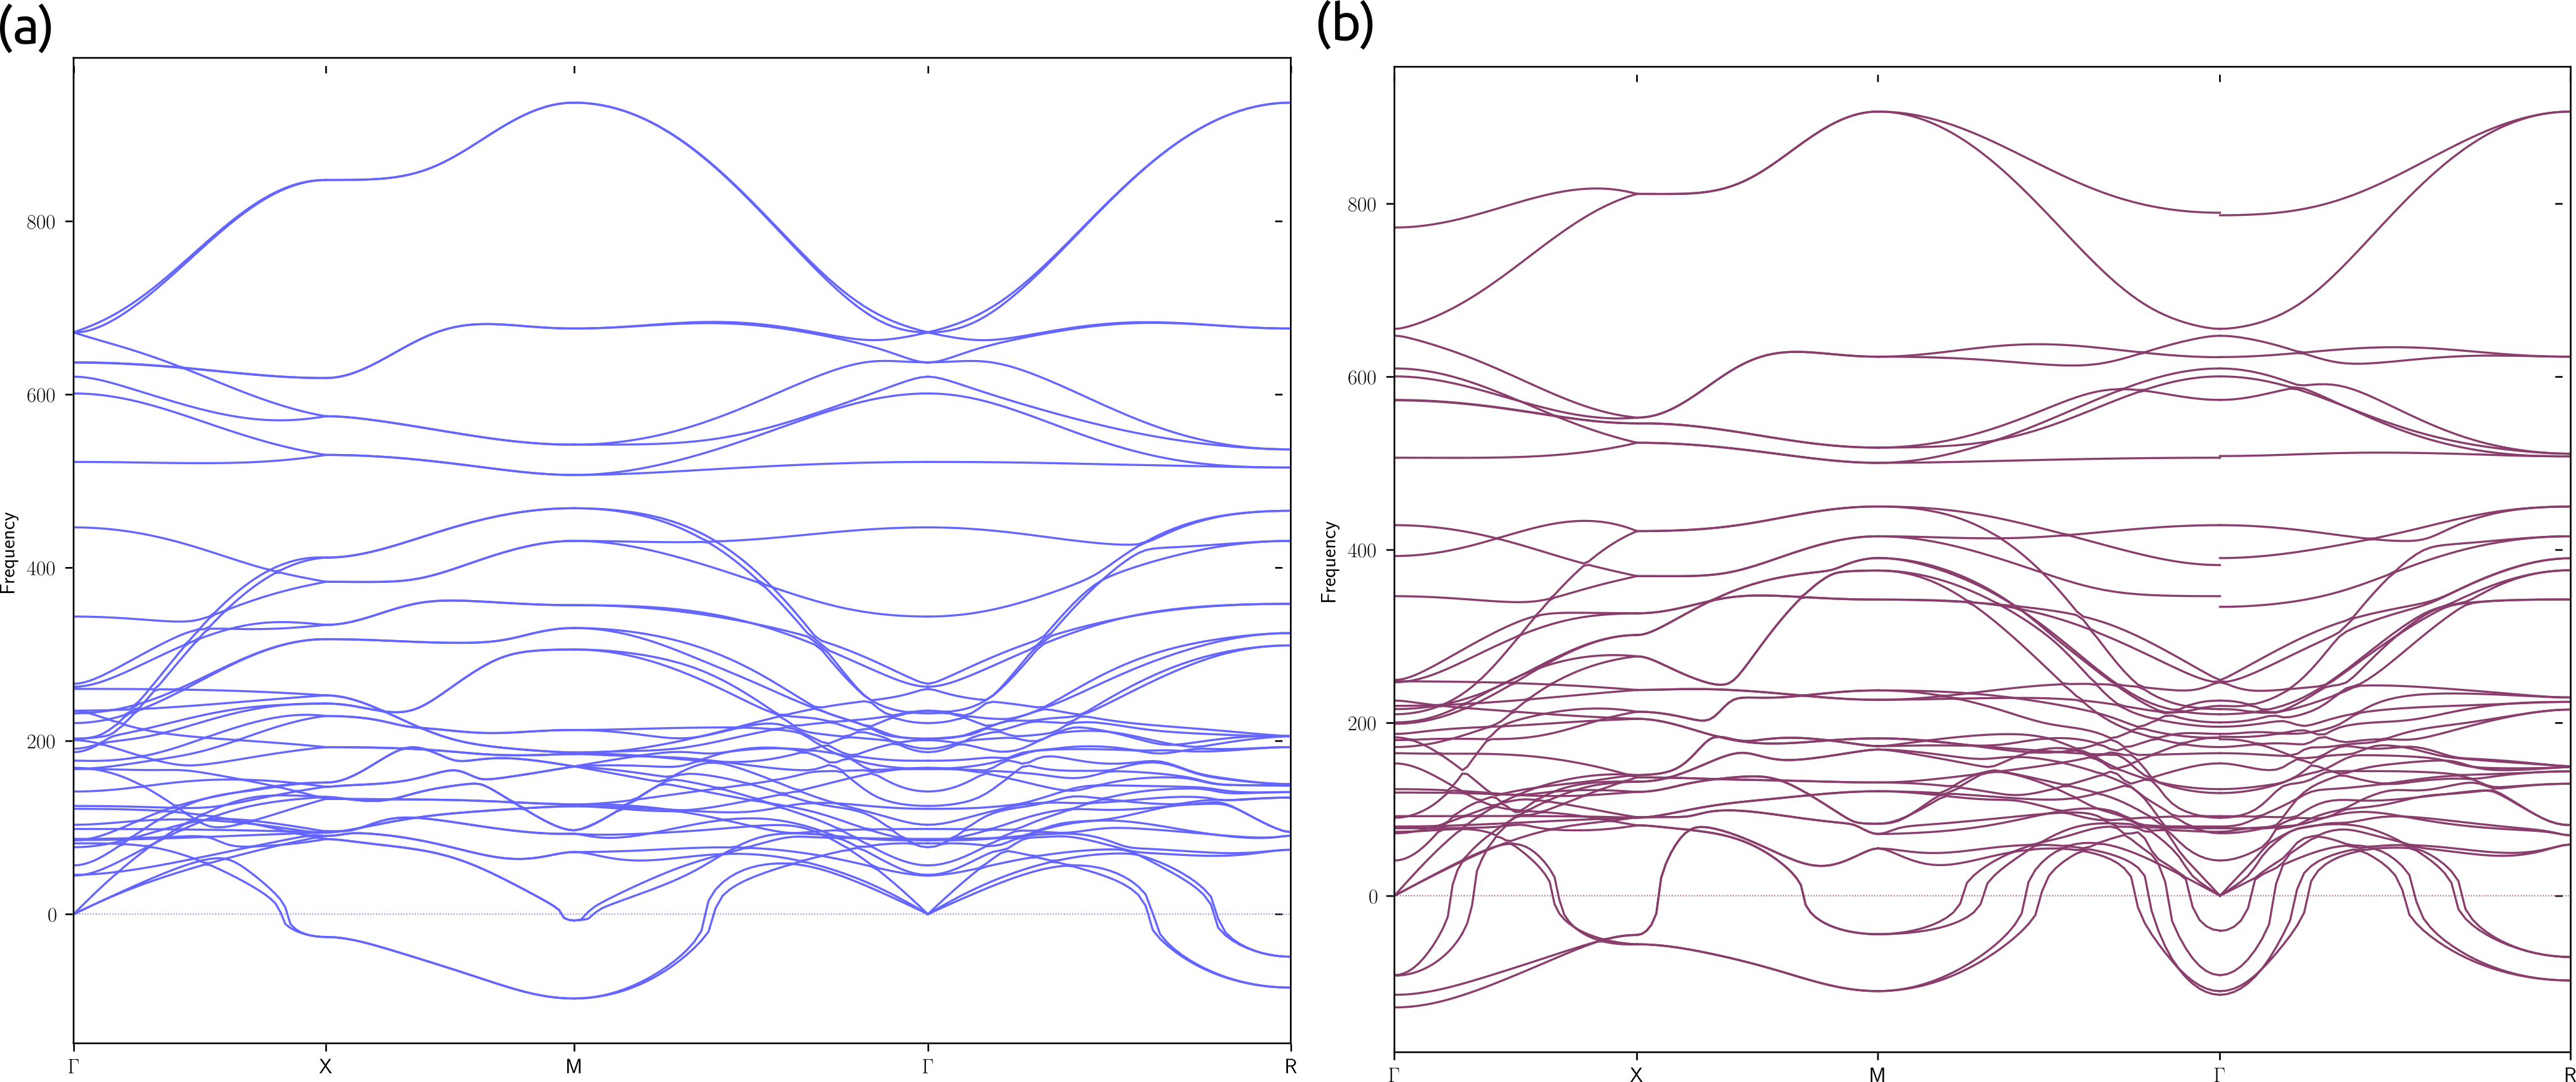
\includegraphics[width=\textwidth]{Figs/dphon-both_trans.png}
    \caption{Dispersión de fonones de la configuración $Immm(71)$ trans (a) $Sr_{2}TaO_{3}N$ y (b) $Sr_{2}NbO_{3}N$.}
    \label{trans-phon}
\end{figure}

Se observa en la dispersión de fonones los 3 modos acústicos que caen en el punto de alta simetría $\Gamma$ de la zona de Brillouin. Esto muestra buenos resultados debido a la corrección no analítica de Wang \cite{Wang_2010-nac} agregada a los cálculos de dispersión de fonones. Sin esta corrección, un modo acústico no cae en el punto $\Gamma$, resultando en solo dos modos acústicos, lo que contradice la teoría de fonones \cite{kaxirasjoannopoulos2019}. Comparando ambas figuras \ref{trans-phon}, se encontró que la estructura $Sr_{2}NbO_{3}N$ tienen modos mas inestables, es decir, de mas baja frecuencia y un numero mayor de modos negativos comparado con la estructura $Sr_{2}TaO_{3}N$. De forma similar sucede en el material tipo perovskita $Sr(Ta,Nb)O_{2}N$ reportado por Gelves \textit{et. al.} \cite{Gelves2021oxynitrides}. Aunque la oxidación en el metal de transición es igual ($Ta^{5+},Nb^{5+}$), la diferencia en los modos inestables puede ser encontrada en la fuerza del enlace entre el metal de transición $(Ta,Nb):5d,4d$ y el nitrógeno $N:2p$, ya que la fuerte interacción covalente conlleva a una ligera mayor repulsión de la nube electrónica, implicando  una mayor inestabilidad de la estructura fonónica \cite{Postnikov1993calculations}. Además, se encontraron modos imaginarios en el punto $\Gamma$ para la estructura $Sr_{2}NbO_{3}N$, lo que no ocurre en la estructura $Sr_{2}TaO_{3}N$.

%no tiene modos imaginarios en el punto de alta simetría $\Gamma$, justamente lo reportado por Gelves \textit{et. al.} \cite{Gelves2021oxynitrides} en la estructura tipo perovskita $SrTaO_{2}N$ 

\subsection{Configuración con ordenamiento tipo \emph{cis}}


Se presenta la curva de dispersión de fonones de las configuraciones \emph{trans-}$Cmcm(63)$ de las estructuras $Sr_{2}TaO_{3}N$ y $Sr_{2}NbO_{3}N$ ilustradas en la figura \ref{cis-phon}(a) y \ref{cis-phon}(b), respectivamente.

\begin{figure}[h!]
    \centering
    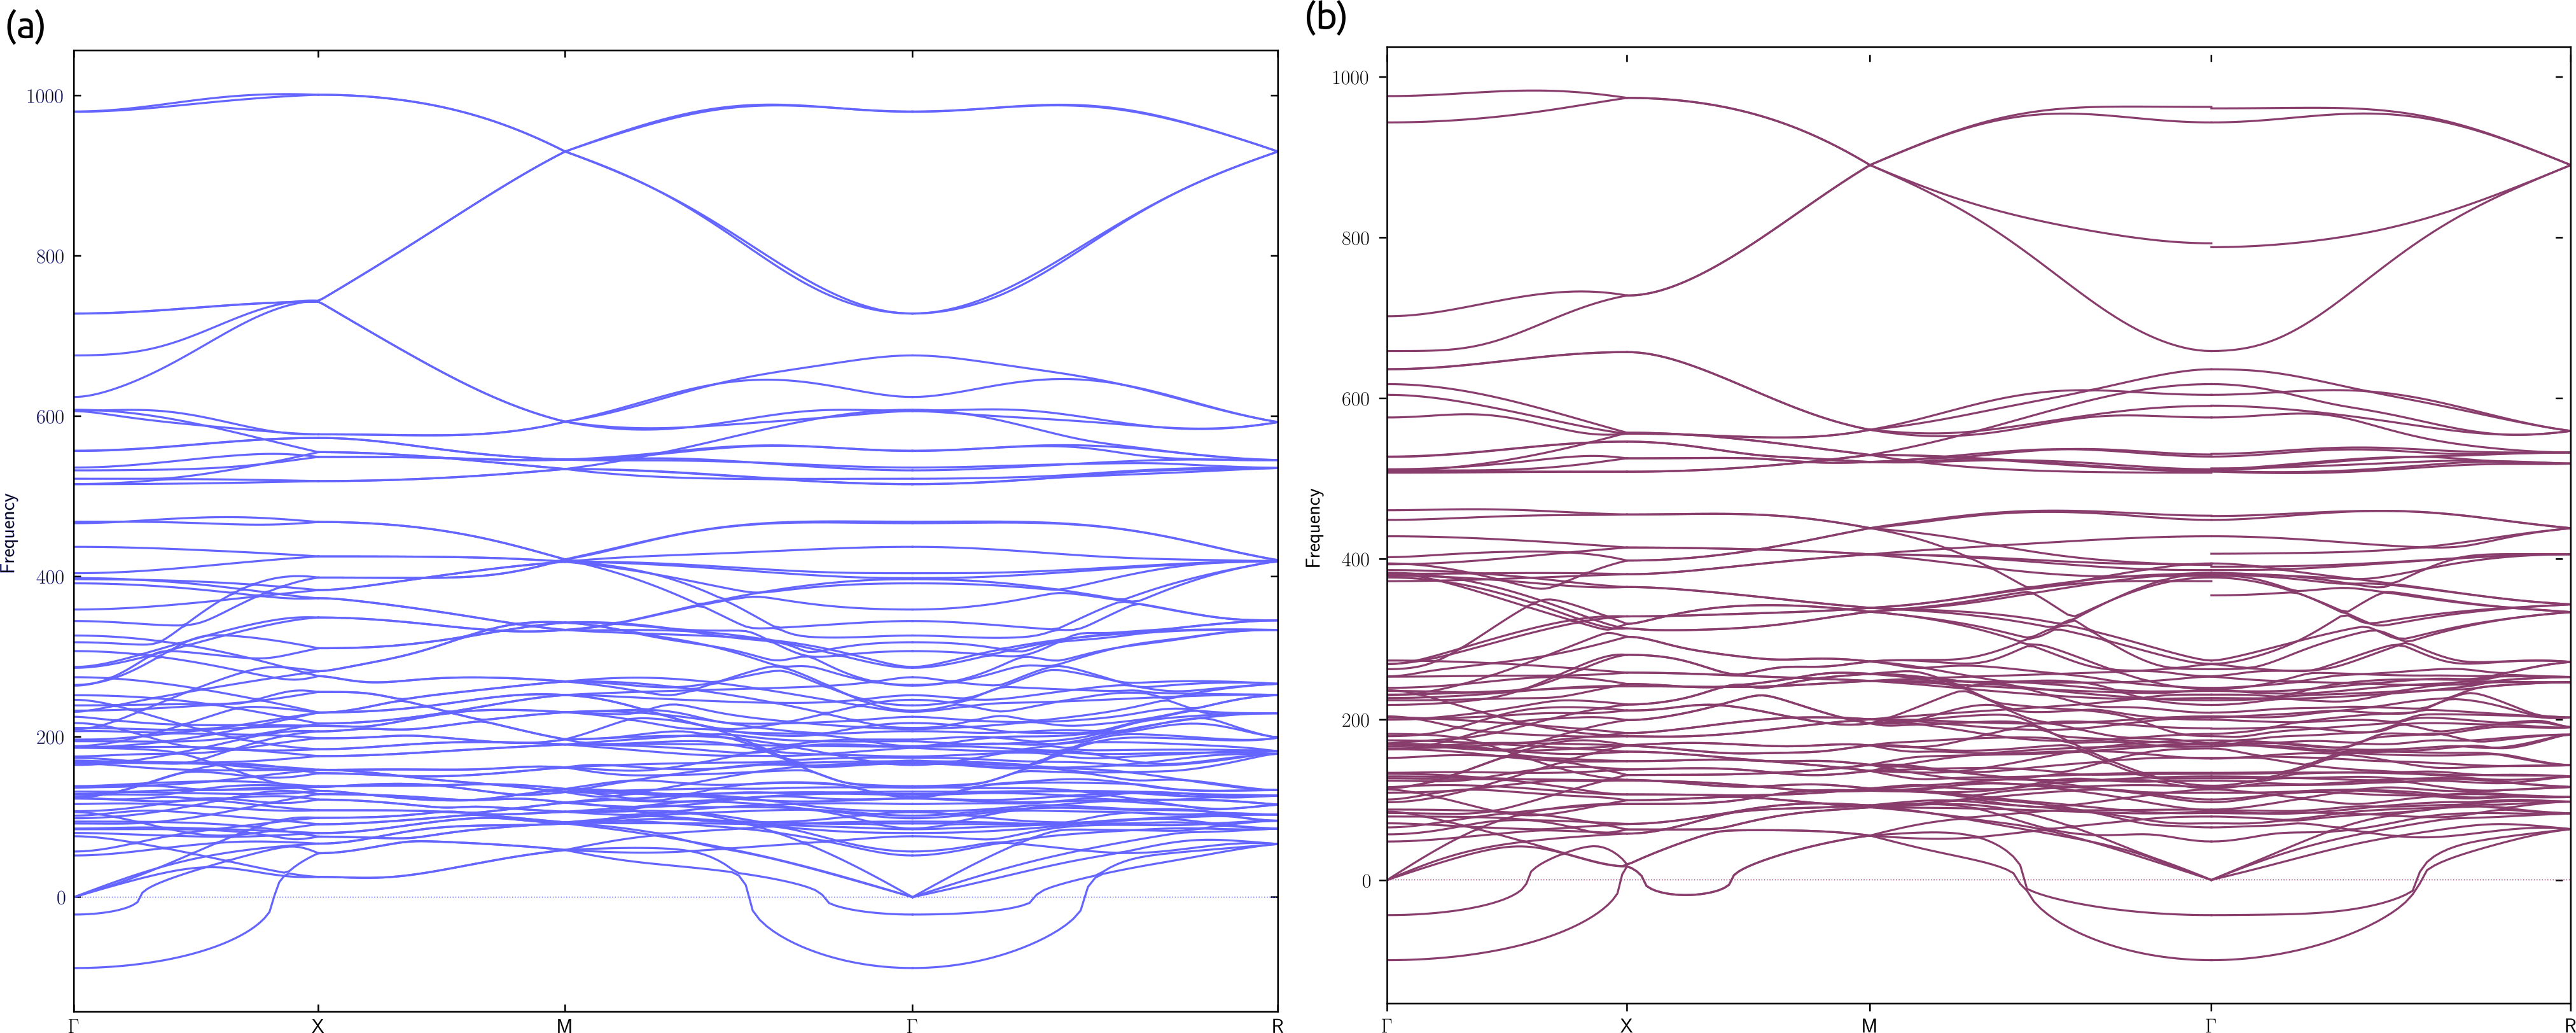
\includegraphics[width=\textwidth]{Figs/dphon-both_cis.png}
    \caption{Dispersión de fonones de la fase $Cmcm(63)$ cis (a) $Sr_{2}TaO_{3}N$ y (b) $Sr_{2}NbO_{3}N$.}
    \label{cis-phon}
\end{figure}

Para el caso de la configuración \emph{cis-}$Sr_{2}TaO_{3}N$ (figura \ref{cis-phon}(a)), la dispersión de fonones muestra 2 modos imaginarios en el punto $\Gamma$ con frecuencias de $-88.45cm^{-1}$ y $-21.74cm^{-1}$. Para el caso de la configuración \emph{cis-}$Sr_{2}NbO_{3}N$ (figura \ref{cis-phon}(b)) se observan 2 modos imaginarios en el punto $\Gamma$ con frecuencias de $-99.93cm^{-1}$ y $-43.86cm^{-1}$. De la misma manera observada en el ordenamiento \emph{trans}, la estructura $Sr_{2}NbO_{3}N$ con orden de aniones \emph{cis} tiene modos imaginarios mas inestables comparados con la estructura $Sr_{2}NbO_{3}N$ con ordenamiento   \emph{cis}. Para este ordenamiento tipo \emph{cis}, solo se encontraron modos imaginarios en el punto de alta simetría $\Gamma$ en la zona de Brillouin, lo que indica un ordenamiento mas estable comparada con la configuración con ordenamiento \emph{trans}. Esto puede deberse a una mas baja energía estructural de la configuración con ordenamiento aniónico \emph{cis} comparado con el ordenamiento aniónico \emph{trans}, como se discutió en el capítulo \ref{Cap. 2}, específicamente en la sección \ref{Sec. 2.2}.

Los modos imaginarios, representados con valores negativos en las figuras \ref{trans-phon} y \ref{cis-phon}, indican inestabilidad estructural a $T=0$, lo que sugiere una ruptura de la simetría en la estructura $Immm(71)$ y $Cmcm(63)$. La estructura puede ser estable con una simetría mas baja o con una celda unitaria diferente. Siguiendo este argumento, los materiales ferroeléctricos son inseparables de la ruptura de la simetría, vienen acompañados de la transición de fase de una estructura centro-simétrica perteneciente a uno de los 32 grupos de punto cristalográfico, a una estructura no centro-simétrica que cae a uno de los 10 grupos de punto ferroeléctrico \cite{Shi2016SymmetryFerroelectrics}. Ahora se puede utilizar la teoría de grupos para explicar la ruptura de simetría causada por distorsiones dadas en la estructura, e identificar si sus combinaciones dan como resultado una simetría polar y luego una posible ferroelectricidad\cite{Yoshida2018HybridPhases}.


\subsection{Diagrama de fases meta-estables para la configuración $Sr_{2}TaO_{3}N$}

Se presenta el diagrama de fases estables y meta-estables para la estructura $Sr_{2}TaO_{3}N$ que contiene los modos inestables encontrados en los ordenamientos \emph{trans} y \emph{cis}. Estos modos imaginarios fueron condensados por el método de \textsc{phonopy} \cite{Togo2015phonopy}, que congela las distorsiones de la estructura encontrando una nueva estructura con menor grupo de simetría. De esta manera se puede analizar las oscilaciones de la nueva estructura encontrada y posteriormente determinar la representación irreducible de cada fonón condensado. La representación irreducible fue encontrada mediante el programa \textsc{amplimodes} \cite{Orobengoa2009amplimodes} para analizar la simetría de las estructuras distorsionadas en base al rompimiento de la simetría de la estructura de alta simetría $Immm(71)$ y $Cmcmc(63)$. 

La figura \ref{Ta-irreps} muestra la diferencia de energía de los modos imaginarios ya condensados comparados con la energía estructural de la configuración principal $Immm(71)$, además de mostrar la representación irreducible de cada modo condensado y las distorsiones (flechas rojas) de la perovskita Ruddlesden-Popper mas estable para cada ordenamiento \emph{trans} y \emph{cis}. De la estructura principal $Sr_{2}TaO_{3}N$ se dividen dos ordenamientos aniónicos \emph{trans} y \emph{cis}, que a su vez se dividen en 5 modos condensados y 2 modos condensados, respectivamente. Se observa que los modos condensados de la configuración con ordenamiento \emph{trans} se posicionan en energía por debajo de la estructura principal $Immm(71)$ y bajan de simetría, encontrando estructuras con grupo espacial $Cmma(67)$, $Pmma(62)$ y $C12/c1(15)$.  El único modo en $X$ tiene grupo espacial $Pmma(62)$ y desplazamiento propio $DT_{4}$. Los modos inestables encontrados en el punto de alta simetría $M$ de la figura \ref{trans-phon}(a) tienen grupo espacial $Cmma(67)$ y representación irreducible $S_{2}^{+}$, incluyendo el modo en $R$ con frecuencia $-49.21cm^{-1}$, pero el otro modo de $R$ tiene grupo espacial $C12/c1(15)$ y desplazamiento propio $T_{2}^{+}$, siendo este el de mas baja energía entre los modos con ordenamiento \emph{trans}, con una diferencia de energía de $-49.4043meV$. Para este modo se ha agregado la estructura cristalográfica a la figura \ref{Ta-irreps}, se aprecian las distorsiones de los octaedros producto de los desplazamientos de los aniones mostrando que los nitrógenos se mueve en sentidos opuestos en dirección [001] con muy poca amplitud de desplazamiento comparado con los oxígenos. Los oxígenos que están en el plano se mueven en sentido opuesto en dirección \emph{'c'}, mientras que los oxígenos del sitio axial se mueven en sentido opuesto sobre el plano en dirección [110].

\begin{figure}[H]
    \centering
    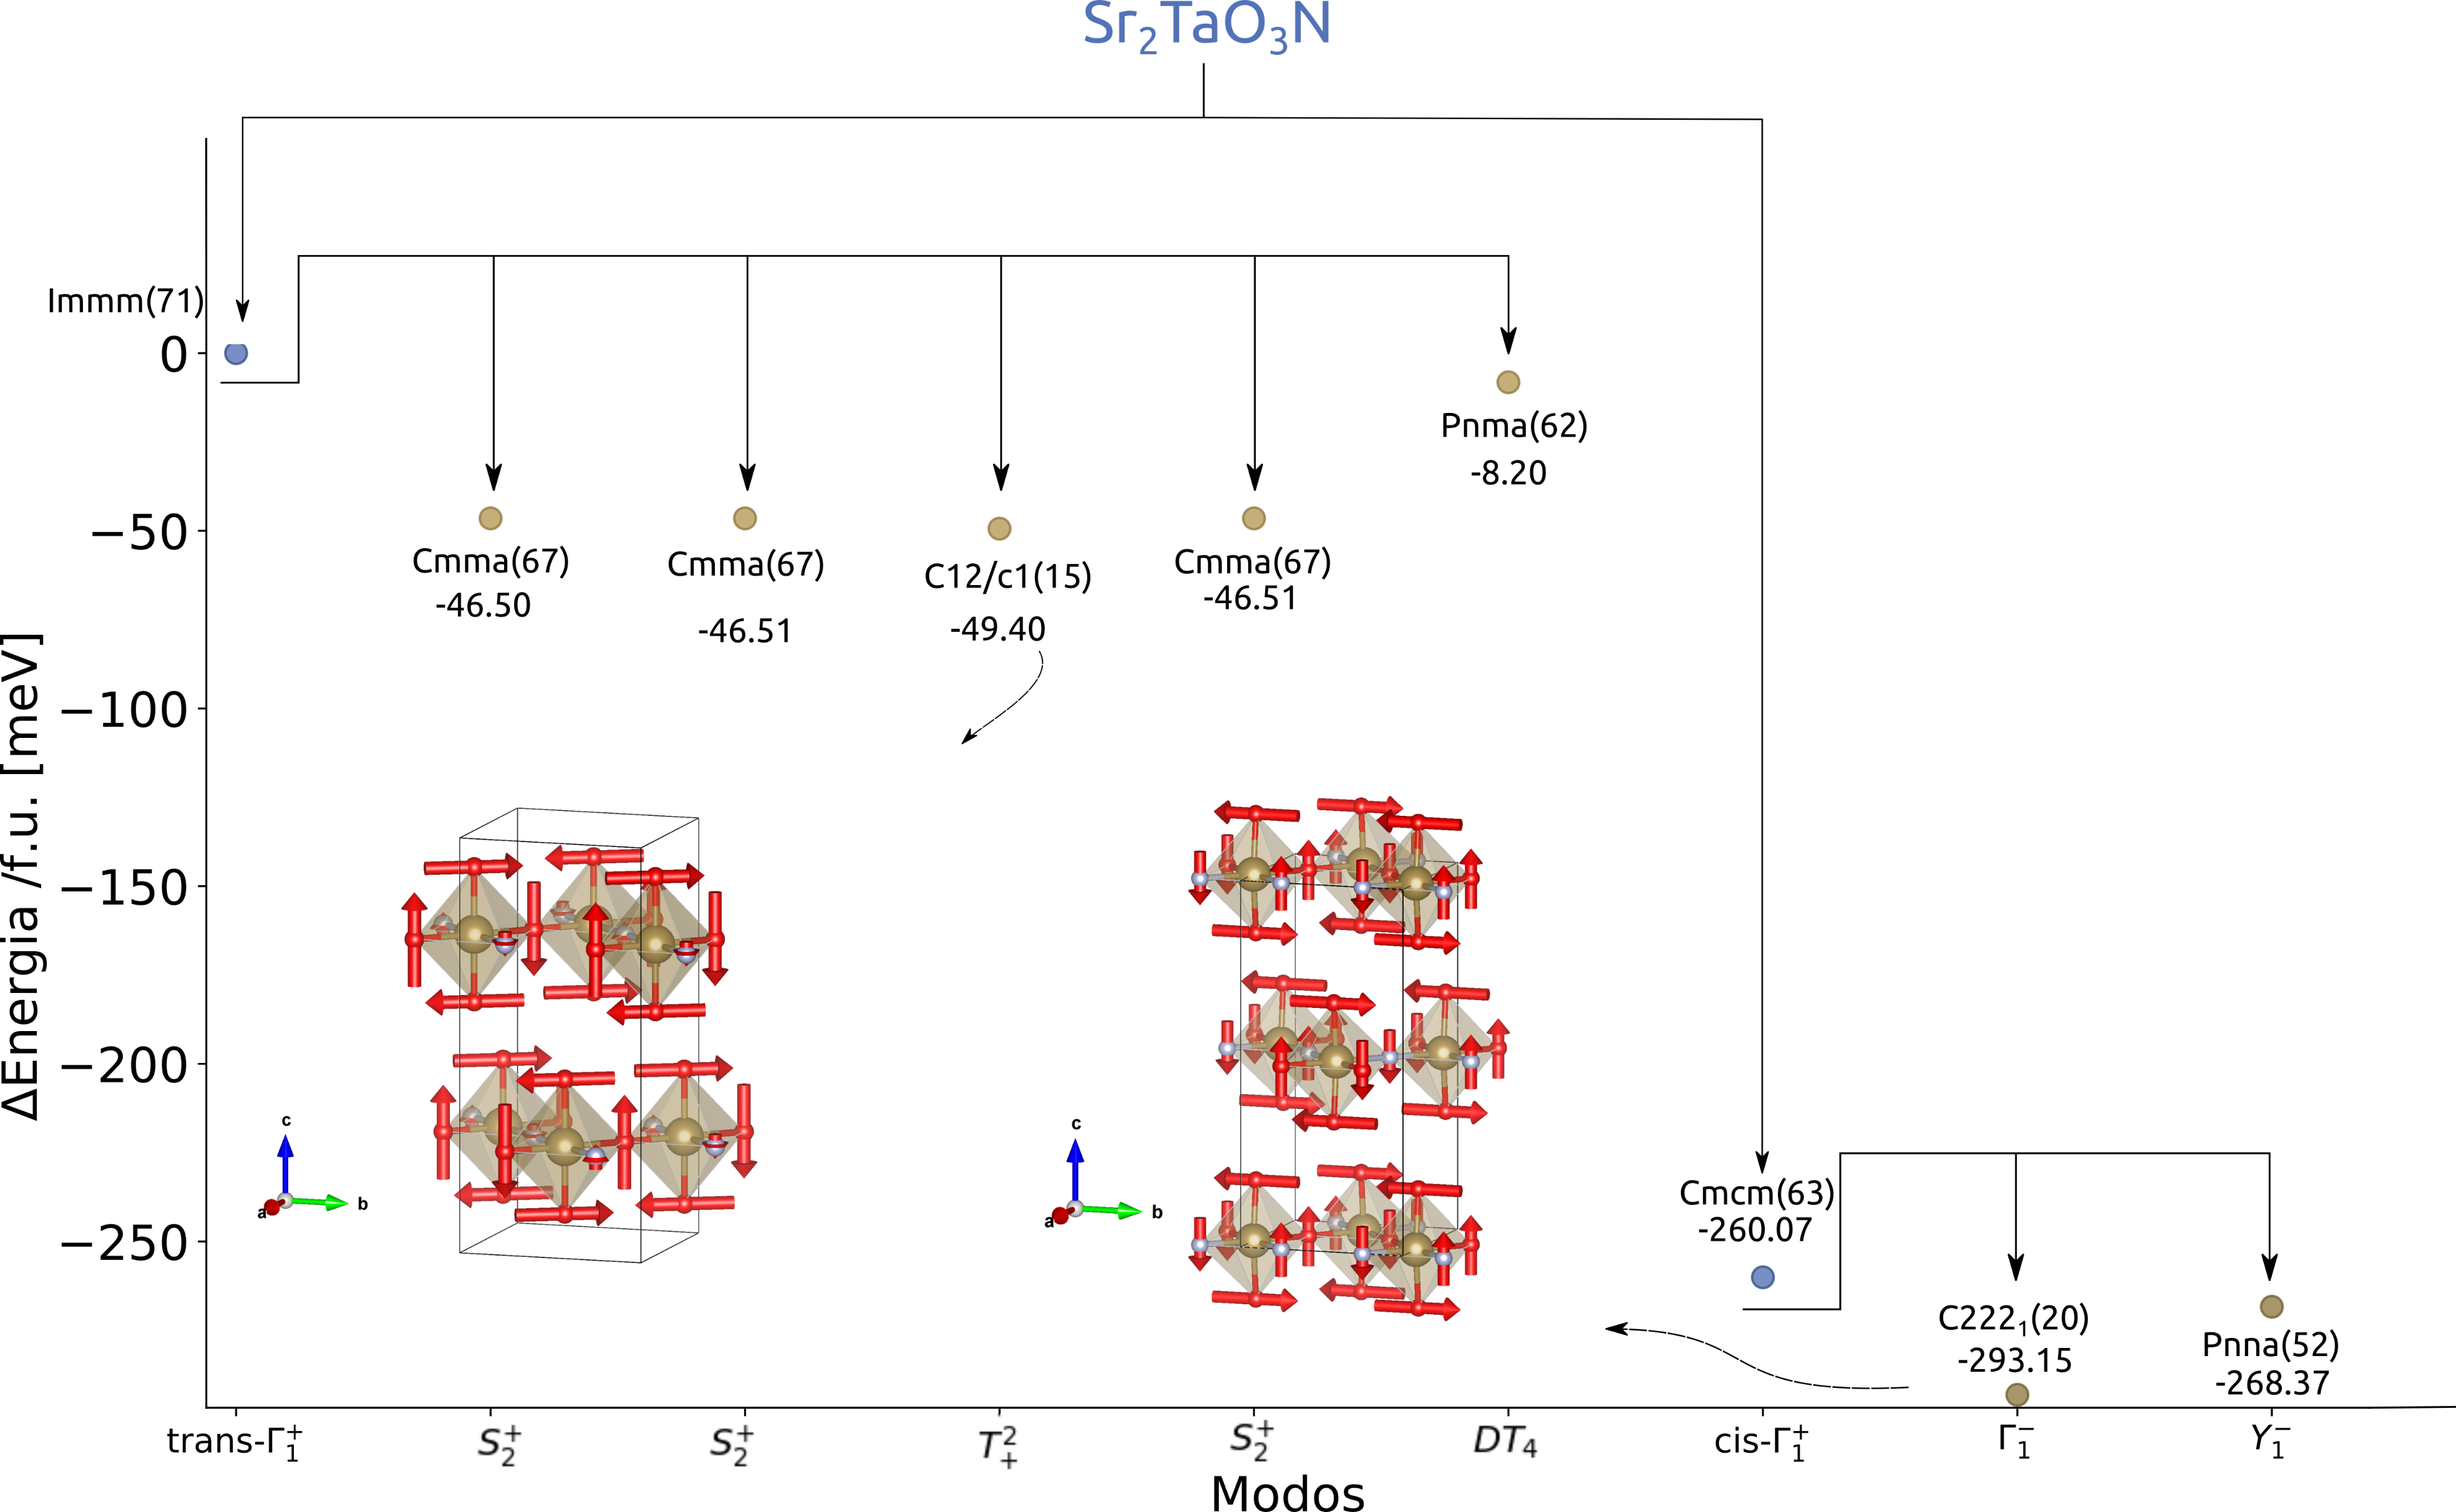
\includegraphics[width=\textwidth]{Figs/Ta-irreps.png}
    \caption{Diagrama de fases meta-estables de $Sr_{2}TaO_{3}N$ para dos principales ordenamientos aniónicos: \emph{trans} y \emph{cis}.}
    \label{Ta-irreps}
\end{figure}

Lo mismo ocurre con los modos condensados de la configuración \emph{cis}, están por debajo en energía y caen a una simetría mas baja que su estructura principal $Cmcm(63)$. La figura \ref{cis-phon}(a) muestra dos modos inestables en $\Gamma$ con grupo espacial $C222_{1}(20)$ y $Pnna(52)$ con desplazamiento propio $\Gamma_{1}^{-}$ y $Y_{1}^{-}$, respectivamente. El modo $\Gamma_{1}^{-}$ es el modo suave encontrado en el diagrama de fases de la estructura $Sr_{2}TaO_{3}N$ (figura \ref{Ta-irreps}),  con una diferencia de energía de $-293.1450meV$. Para este modo se ha agregado la estructura cristalográfica a la figura \ref{Ta-irreps}, se aprecian las distorsiones de los octaedros producto de los desplazamientos de los aniones mostrando que un nitrógeno se mueve en un sentido en dirección [001], el otro nitrógeno se mueve en el sentido opuesto, pero en la misma dirección. Lo mismo sucede con los oxígenos en el plano, mientras que los oxígenos del sitio axial se mueven sobre el plano en sentidos opuesto con una ligera mayor amplitud en los desplazamientos. 

\subsection{Diagrama de fases meta-estables para la configuración $Sr_{2}NbO_{3}N$}

Se presenta el diagrama de fases estables y meta-estables para la estructura $Sr_{2}NbO_{3}N$ que contiene los modos inestables encontrados en los ordenamientos \emph{trans} y \emph{cis}. Asi como en el diagrama de fases de la figura \ref{Ta-irreps}, la figura \ref{Nb-irreps} muestra los modos imaginarios condensados por el método de \textsc{phonopy} \cite{Togo2015phonopy}, la representación irreducible fue encontrada mediante el programa \textsc{amplimodes} \cite{Orobengoa2009amplimodes} para analizar la simetría de las estructuras distorsionadas en base al rompimiento de la simetría de la estructura de alta simetría $Immm(71)$ y $Cmcmc(63)$. 


La figura \ref{Nb-irreps} muestra la diferencia de energía de los modos imaginarios ya condensados comparados con la energía estructural de la configuración principal $Immm(71)$, además de mostrar la representación irreducible de cada modo condensado y las distorsiones (flechas rojas) de la perovskita Ruddlesden-Popper mas estable para cada ordenamiento \emph{trans} y \emph{cis}. De la estructura principal $Sr_{2}NbO_{3}N$ se dividen dos ordenamientos aniónicos \emph{trans} y \emph{cis}, que a su vez se dividen en 10 modos condensados y 2 modos condensados, respectivamente. Se observa que los modos condensados de la configuración con ordenamiento \emph{trans} se posicionan en energía por debajo de la estructura principal $Immm(71)$ y bajan de simetría. Dos modos condensados en $\Gamma$ muestran grupo de simetría $Imm2(44)$ con desplazamiento propio $\Gamma_{2}^{-}$ y $\Gamma_{4}^{-}$, respectivamente; mientras que los otros dos modos $Pmmn(59)$ con desplazamiento propio $X_{2}^{-}$ y $X_{4}^{-}$, respectivamente. Los dos modos encontrados en $X$ muestran grupo de simetría $Pmna(62)$ con desplazamiento propio $DT_{4}$ y $DT_{3}$, respectivamente. Los modos encontrados en $M$ y $R$ muestran el mismo desplazamiento propio $S_{2}^{+}$ con grupo de simetría $Cmma(67)$, $P121(3)$, $P12/c1(13)$ y $C12/c1(15)$. Este ultimo modo es el de mas baja energía entre los modos con ordenamiento \emph{trans}, con una diferencia de energía de $-73.3126meV$. Para este modo se ha agregado la estructura cristalográfica a la figura \ref{Nb-irreps}, se aprecian las distorsiones de los octaedros producto de los desplazamientos de los aniones mostrando que los nitrógenos se mueve en sentidos opuestos en dirección [001] con una mayor amplitud de desplazamiento comparado con los oxígenos. Los oxígenos que están en el plano se mueven en sentido opuesto en dirección [001], mientras que los oxígenos del sitio axial se mueven en sentido opuesto sobre el plano en dirección [110].

\begin{figure}[H]
    \centering
    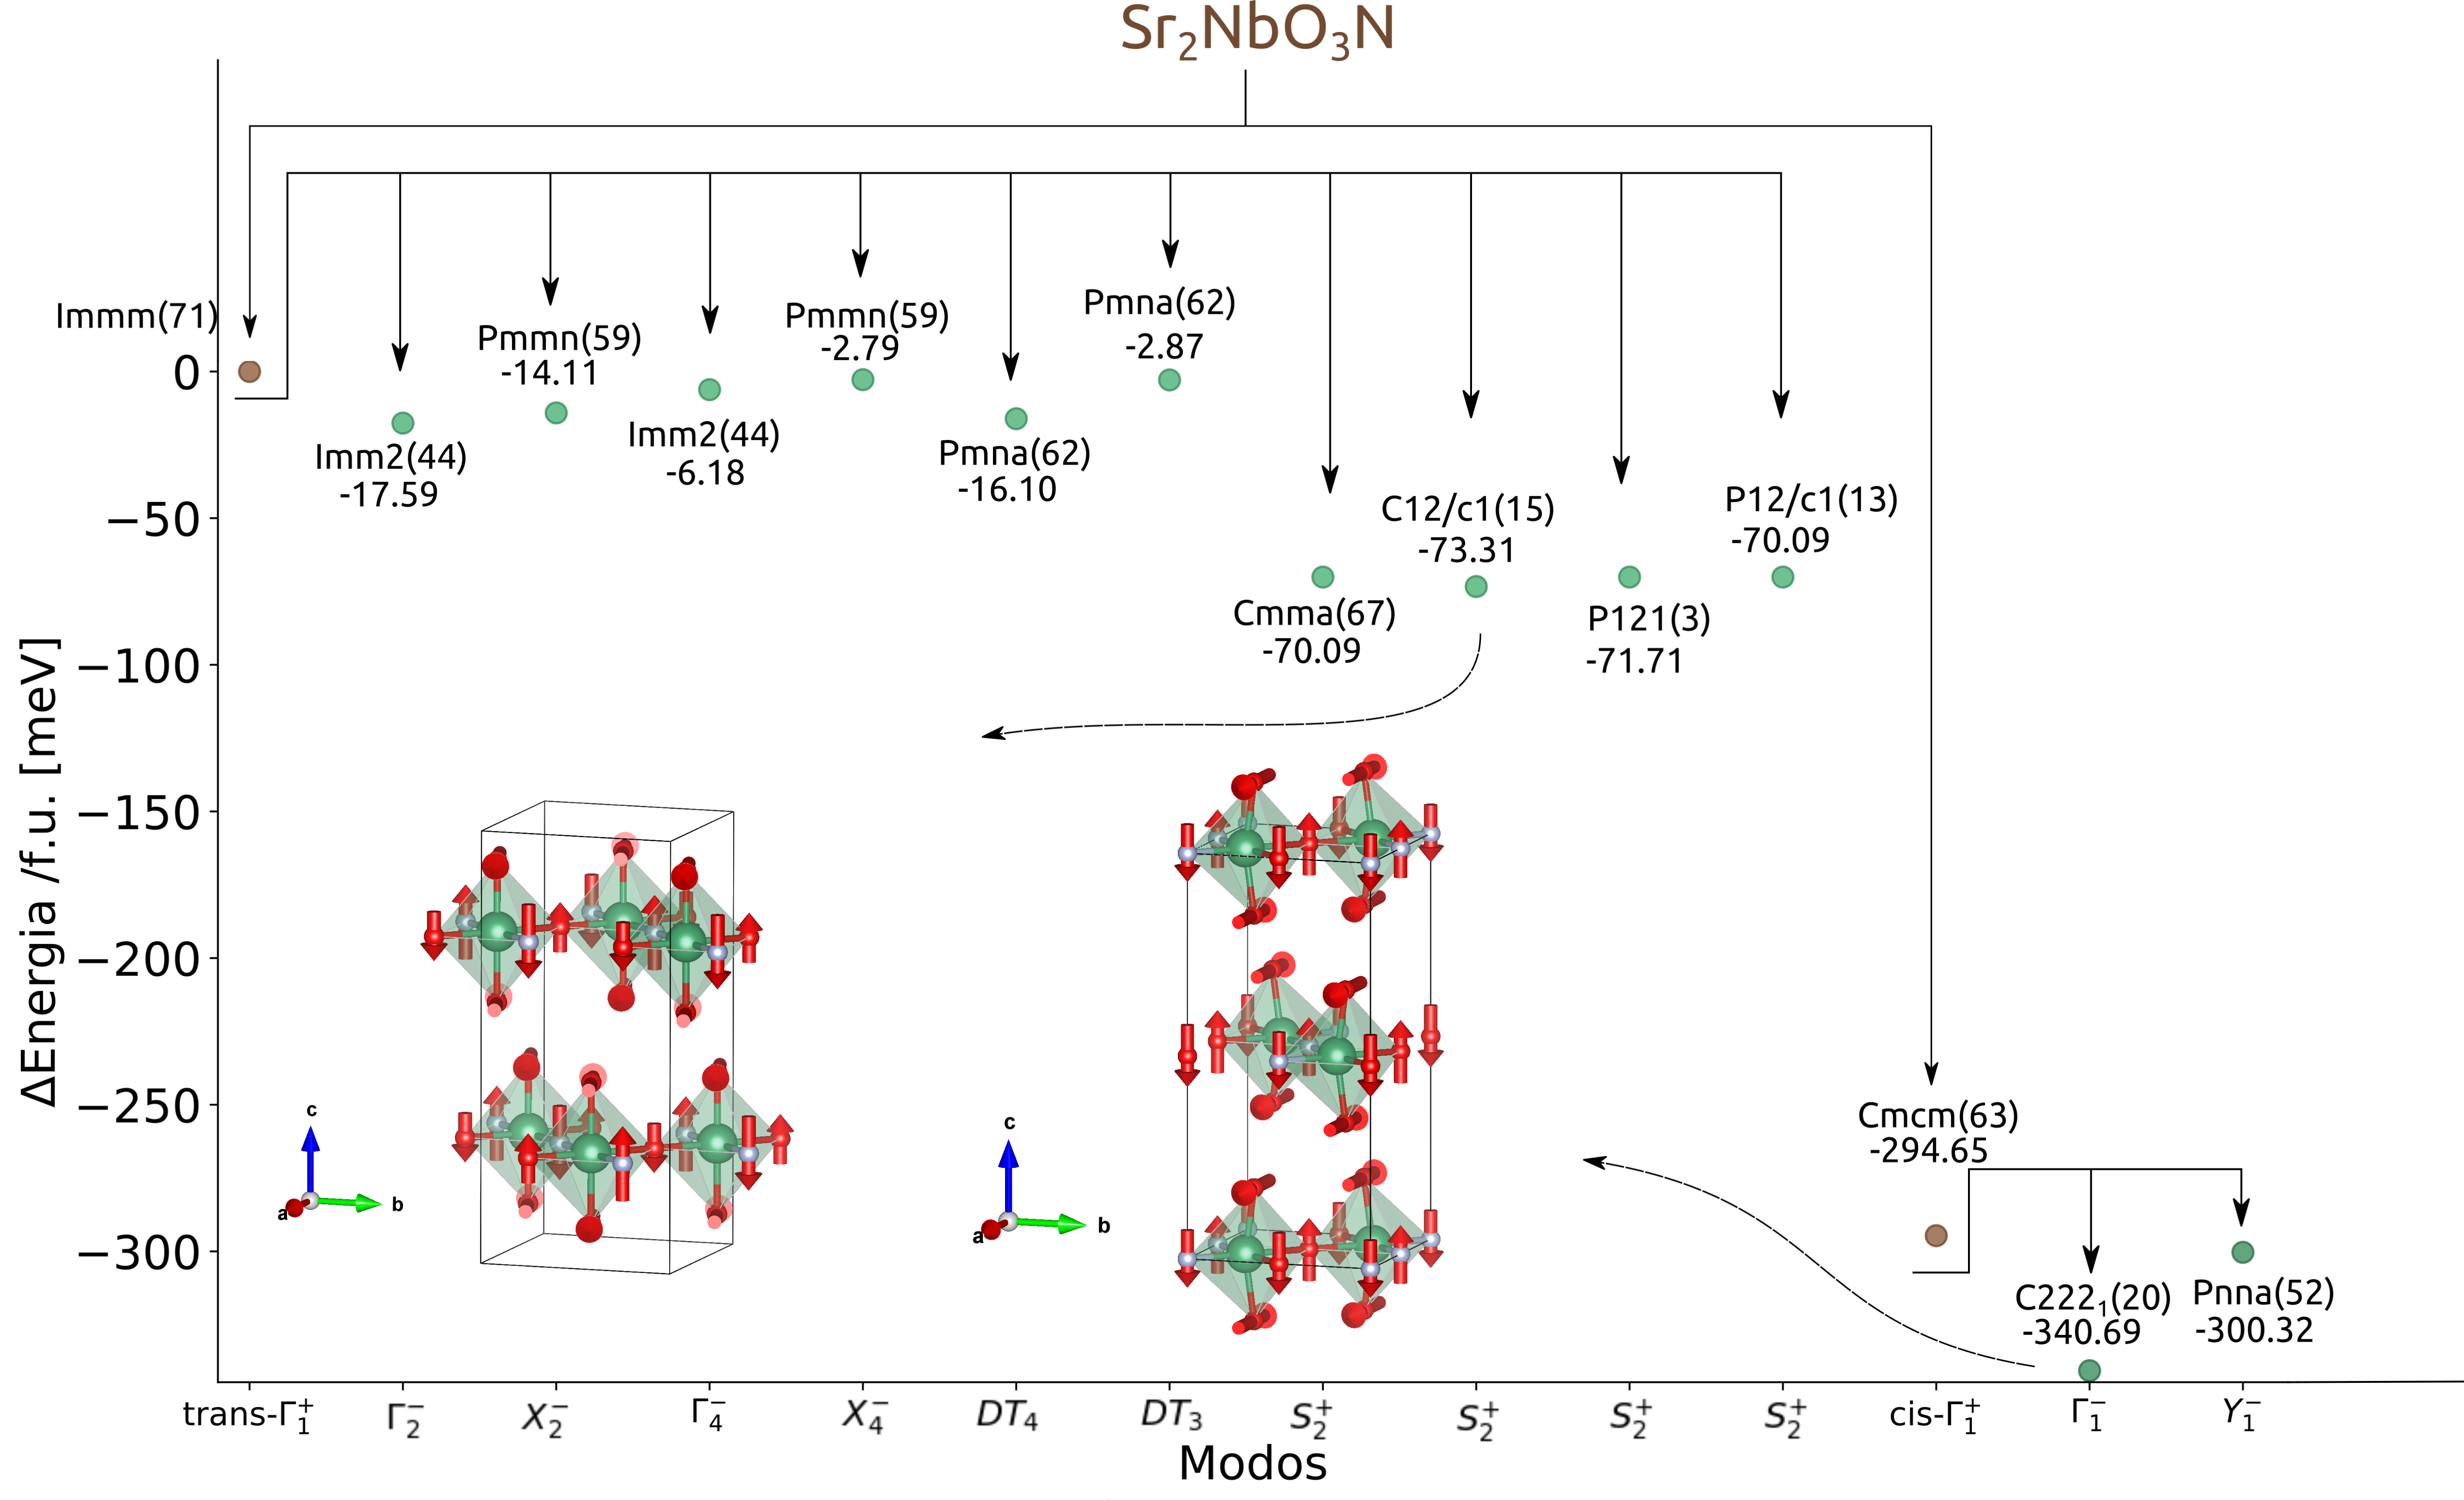
\includegraphics[width=\textwidth]{Figs/Nb-irreps.png}
    \caption{Diagrama de fases meta-estables de $Sr_{2}NbO_{3}N$ de dos principales ordenamientos aniónicos: \emph{trans} y \emph{cis}.}
    \label{Nb-irreps}
\end{figure}

Lo mismo ocurre con los modos condensados de la configuración \emph{cis}, están por debajo en energía y caen a una simetría mas baja que su estructura principal $Ccmmc(63)$. La figura \ref{cis-phon}(b) muestra dos modos inestables en $\Gamma$ con grupo espacial $C222_{1}(20)$ y $Pnna(52)$ con desplazamiento propio $\Gamma_{1}^{-}$ y $Y_{1}^{-}$, respectivamente. El modo $\Gamma_{1}^{-}$ es el modo suave encontrado en el diagrama de fases de la estructura $Sr_{2}NbO_{3}N$ (figura \ref{Nb-irreps}),  con una diferencia de energía de $-340.6840meV$. Para este modo se ha agregado la estructura cristalográfica a la figura \ref{Nb-irreps}, se aprecian las distorsiones de los octaedros producto de los desplazamientos de los aniones mostrando que un nitrógeno se mueve en un sentido en dirección [001], el otro nitrógeno se mueve en el sentido opuesto, pero en la misma dirección. Lo mismo sucede con los oxígenos en el plano, mientras que los oxígenos del sitio axial se mueven sobre el plano en sentidos opuesto. 

Para ambos casos, en las figuras \ref{Ta-irreps} y \ref{Nb-irreps} se observa que la configuración energéticamente mas favorable tiene un orden de aniones \emph{cis} en el plano (ab) y exhibe rotaciones octaédricas tanto en $NbO_{4}N_{2}$ como en $TaO_{4}N_{2}$, lo que esta en concordancia con lo reportado en la literatura \cite{Bouri2018}. La ferroelectricidad puede darse en materiales no-centro-simétricos que pertenezcan a alguno de los 10 grupos de punto polar con dos estados de orientación \cite{Rabe2007ModernFerro}, como lo denota Gelves \textit{et. al.} \cite{Gelves2021oxynitrides} en el doble pozo (ó en inglés \textit{double well}) del material tipo perovskita $Sr(Ta,Nb)O_{2}N$. En este sentido, el modo suave encontrado en ambos materiales tiene el grupo espacial $C222_{1}$ (S.G. 20), el cual pertenece al grupo de punto $222$ según la notación de Herrmann-Mauguin \cite{Hermann2015notation}. En el anexo \ref{anexoC} se aprecian los 10 grupos de punto polar, así que el grupo de punto $222$ no es un material polar. Sin embargo, se ha encontrado que este grupo pertenece al grupo de punto enantiomórfo (ver tabla \ref{Tab. quiral}), lo que indica que el material es un material quiral.






%%%%%%%%%%%%%%%%%%%%%%%%%%%%%%%%%%%% leer para agregar en el marco teorico de phonons    %https://mattermodeling.stackexchange.com/questions/3657/what-do-negative-phonon-frequencies-signify
 % Trabajo futuro
% ------------------------------------------------------------------------
% ------------------------------------------------------------------------
% ------------------------------------------------------------------------
%                             Conclusiones
% ------------------------------------------------------------------------
% ------------------------------------------------------------------------
% ------------------------------------------------------------------------

\chapter{RECOMENDACIONES Y TRABAJO FUTURO}
% ------------------------------------------------------------------------

Como se pudo apreciar en la estructura electrónica de la configuración con ordenamiento \emph{trans-}$Sr_{2}(Ta,Nb)O_{3}N$ y grupo espacial $Immm$ (S.G. 71), los resultados de la brecha entre la banda de conducción y la banda de valencia en el punto de alta simetría $\Gamma$ no son acordes a los reportes en la literatura \cite{Cen2019OptimizedSplitting,Clarke2002,Bouri2018}, obteniendo una brecha mucho menor a lo esperado. Esto sugiere un aumento del parámetro \textsc{u} mayor a $4eV$ con el fin de subir en energía las bandas del metal de transición, y así lograr resultados mas acordes a la literatura.

Por otro lado, se encontró que la fase $Sr_{2}(Ta,Nb)O_{3}N$ con ordenamiento aniónico \emph{cis}, desplazamiento propio $\Gamma_{1}^{-}$ y grupo espacial $C222_{1}$ (S.G. 20), no hace parte del grupo de punto polar, indicando que no es un material ferroeléctrico. Sin embargo, se sugiere realizar cálculos de primeros principios para analizar si el material puede tener un doble pozo, además de sugerir la medición de la polarización espontánea. Un resultado interesante es la mención de que el material pertenece al grupo de punto enantomórfo, lo que sugiere sea un material quiral. Los materiales quirales se distinguen por no poder superponerse a su imagen espejo
\cite{milic2021Multi}, es decir, sus operaciones de simetría no contienen ejes de rotación impropios. Estos materiales son muy deseados por sus aplicaciones en spintrónica y quiroptoelectrónica debido al fuerte acoplamiento espín-orbita y controlable dispersión Rashba \cite{milic2021Multi}.






\chapter{CONCLUSIONES}

En este trabajo de grado se investigaron de manera computacional y en el marco de la materia condensada y la teoría funcional de la densidad las propiedades estructurales, electrónicas y fonónicas del material perovskita tipo Ruddlesden-Popper $Sr_{2}(Ta,Nb)O_{3}N$, además de reportar la necesidad de introducir la teoría del campo medio dinámico (por sus siglas es inglés \textsc{dmft}) a la estructura $Sr_{2}(Ta,Nb)O_{3.5}N_{0.5}$.

Se encontraron once configuraciones con diferente ordenamiento aniónico para el material $Sr_{2}(Ta,Nb)O_{3}N$, y dos configuraciones para el material $Sr_{2}(Ta,Nb)O_{3.5}N_{0.5}$.  Se comprendió la discrepancia sobre la energía estructural mas favorable entre los ordenamientos aniónicos \emph{trans} y \emph{cis}, concluyendo que el problema radicaba en una cuestión de simetría para que el orden \emph{cis} se diera en estos materiales, siendo este el ordenamiento mas favorable con energia de $-55.41eV$ y $-52.16eV$ para $Sr_{2}TaO_{3}N$ y $Sr_{2}NbO_{3}N$, respectivamente. Se pudo apreciar el papel que juega el parámetro \textsc{u}$=4eV$ en elementos altamente correlacionados como el tántalo y el niobio, obteniendo energías estructurales y bandas electrónicas mas acordes a lo reportado en la literatura.

En la estructura electrónica de las configuraciones $Immm(71)$ y $Cmcm(63)$ se encontró el posicionamiento del metal de transición en las bandas de conducción, mientras que las bandas de valencia son ocupadas por el nitrógeno, disminuyendo la  brecha directa en el punto $\Gamma$ de alta simetría en la zona de Brillouin, lo que hace a este material favorable para la división de agua mediante fotocatálisis.

Al realizar la curva de dispersión de fonones, se encontraron mas modos inestables en el orden \emph{cis} comparado con el orden \emph{trans}, además de hallar el modo mas estable después de condensar los modos imaginarios, concluyendo que el desplazamiento propio es $\Gamma_{1}^{-}$ con grupo espacial $C222_{1}$ (S.G. 20). Aunque este grupo no pertenece a los grupos de punto polar, hace parte del grupo de punto quiral, abriendo la puerta al análisis de sus características estructurales.

Cabe resaltar que los resultados de esta investigación fueron presentados como poster en el congreso internacional \textsc{virtual mrs spring meeting $\&$ exhibit} en abril del 2021, con el título \textit{EL09.07.05: THEORETICAL INVESTIGATION OF THE ELECTRONIC PROPERTIES OF RUDDLESDEN-POPPER Sr$_{2}$AO$_{4-x}$N$_{x}$(A=Nb,Ta)(x=1.0)}.






% ------------------------------------------------------------------------
% ------------------------------------------------------------------------
 % Conclusiones
% ------------------------------------------------------------------------
% Bibliografía
% ------------------------------------------------------------------------
%\printbibliography[heading=bibintoc,title={BIBLIOGRAFÍA},omitnumbers=true]
% ------------------------------------------------------------------------
% Anexos
% ------------------------------------------------------------------------
% ------------------------------------------------------------------------
% ------------------------------------------------------------------------
% ------------------------------------------------------------------------
%                                Anexo A
% ------------------------------------------------------------------------
% ------------------------------------------------------------------------
% ------------------------------------------------------------------------
% ------------------------------------------------------------------------
\nnchapter{ANEXOS}
% ------------------------------------------------------------------------
\anexo{Operaciones de simetría del grupo cristalográfico \emph{I4/mmm} (139)}\label{anexoA}

El programa \textsc{sod} usa dos archivos de entrada para realizar las substituciones, el archivo \textsc{'insod'} y el archivo \textsc{sgo}. Este anexo esta enfocado en el segundo archivo \textsc{'sgo'}, por sus siglas en inglés \textbf{'s}\textit{ymmtry} \textbf{g}\textit{roup} \textbf{o}\textit{perator'}.\\

Los grupos espaciales están numerados del $1$ al $230$ y están ordenados según los $7$ sistemas cristalinos: triclínico, monoclínico, ortorrómbico, tetragonal, trigonal, hexagonal y cúbico. El archivo \textsc{sgo} contiene todas las operaciones de simetría del grupo espacial cristalográfico. Cada grupo espacial tiene asociado un número único que es independiente de la elección de la celda unitaria ó del etiquetado de los ejes\cite{urlcsgdt}. En el caso de la estructura inicial \textsc{rp}-$Sr_{2}BO_{4}(B=Ta/Nb)$, el grupo espacial que le corresponde es \textit{I4/mmm}, el número que le corresponde a este grupo espacial es el 139. Dentro del grupo espacial hay $32$ operaciones de simetría que el programa \textsc{sod} debe leer usando el archivo \textsc{sgo}. Las $32$ operaciones de simetría son:

\begin{align*}
        1.\quad& x,y,z                  & 9.\quad& \bar{x},\bar{y},\bar{z}  & 17.\quad& x+\frac{1}{2},y+\frac{1}{2},z+\frac{1}{2}   & 25.\quad& \bar{x}+\frac{1}{2},\bar{y}+\frac{1}{2},\bar{z}+\frac{1}{2}\\
        2.\quad& \bar{x},\bar{y},z      & 10.\quad& x,y,\bar{z}             & 18.\quad& \bar{x}+\frac{1}{2},\bar{y}+\frac{1}{2},z+\frac{1}{2}      & 26.\quad& x+\frac{1}{2},y+\frac{1}{2},\bar{z}+\frac{1}{2}\\
        3.\quad& \bar{y},x,z            & 11.\quad& y,\bar{x},\bar{z}       & 19.\quad& \bar{y}+\frac{1}{2},x+\frac{1}{2},z+\frac{1}{2}            & 27.\quad& y+\frac{1}{2},\bar{x}+\frac{1}{2},\bar{z}+\frac{1}{2} \\
        4.\quad& y,\bar{x},z            & 12.\quad& \bar{y},x,\bar{z}       & 20.\quad& y+\frac{1}{2},\bar{x}+\frac{1}{2},z+\frac{1}{2}            & 28.\quad& \bar{y}+\frac{1}{2},x+\frac{1}{2},\bar{z}+\frac{1}{2} \\
        5.\quad& \bar{x},y,z            & 13.\quad& x,\bar{y},\bar{z}       & 21.\quad& \bar{x}+\frac{1}{2},y+\frac{1}{2},z+\frac{1}{2}            & 29.\quad& x+\frac{1}{2},\bar{y}+\frac{1}{2},\bar{z}+\frac{1}{2} \\
        6.\quad& x,\bar{y},z            & 14.\quad& \bar{x},y,\bar{z}       & 22.\quad& x+\frac{1}{2},\bar{y}+\frac{1}{2},z+\frac{1}{2}            & 30.\quad& \bar{x}+\frac{1}{2},y+\frac{1}{2},\bar{z}+\frac{1}{2}\\
        7.\quad& y,x,z                  & 15.\quad& \bar{y},\bar{x},\bar{z} & 23.\quad& y+\frac{1}{2},x+\frac{1}{2},z+\frac{1}{2}                  & 31.\quad& \bar{y}+\frac{1}{2},\bar{x}+\frac{1}{2},\bar{z}+\frac{1}{2}   \\
        8.\quad& \bar{y},\bar{x},z      & 16.\quad& y,x,\bar{z}             & 24.\quad& \bar{y}+\frac{1}{2},\bar{x}+\frac{1}{2},z+\frac{1}{2}      & 32.\quad& y+\frac{1}{2},x+\frac{1}{2},\bar{z}+\frac{1}{2}       
\end{align*}


Cada operación de simetría representa una matriz diferente. Las primeras $16$ operaciones de simetría son matrices de rotación. Las faltantes $16$ operaciones de simetría son matrices de rotación y un vector de traslación. La operación de simetría numero 1 es una matriz diagonal:

\begin{equation*}
    \begin{bmatrix}
     1& 0 &0 \\ 
     0& 1 & 0\\ 
     0& 0 & 1
    \end{bmatrix} 
\end{equation*} 

La operación de simetría numero $4. y,\bar{x},z$ tiene dos cambios respecto a la primera: la barra encima de la componente ($\bar{x}$) significa que el valor de esa columna es negativa; y el segundo cambio es que las componentes cambia de posición, pasan de ser $\bar{x},y,z$ a ser $y,\bar{x},z$. En una matriz, la operacion de simetria $4$ es:

\begin{equation*}
    \begin{bmatrix}
     0& -1 &0 \\ 
     1& 0 & 0\\ 
     0& 0 & 1
    \end{bmatrix} 
\end{equation*} 

Ahora, la operación de simetría numero $32. y+\frac{1}{2},x+\frac{1}{2},\bar{z}+\frac{1}{2}$ tiene una operacional adicional de translación, es decir, un vector columna de traslación:

\begin{equation*}
    \begin{bmatrix}
     0& 1 &0 \\ 
     1& 0 & 0\\ 
     0& 0 & -1
    \end{bmatrix}\begin{bmatrix}
     0.5 \\
     0.5 \\
     0.5
    \end{bmatrix} 
\end{equation*} 


El programa \textsc{sod} realiza cada una de las $32$ operaciones de simetría a las estructuras \textsc{rp}-$Sr_{2}BO_{3.5}N_{0.5}$ y \textsc{rp}-$Sr_{2}BO_{3}N$ teniendo en cuenta las concentración de nitrógeno. Al final el programa define que configuraciones de ocupación aniónica son posibles.
% ------------------------------------------------------------------------
 % Fundamentos de sólidos rígidos
% ------------------------------------------------------------------------
% ------------------------------------------------------------------------
% ------------------------------------------------------------------------
%                                Anexo B
% ------------------------------------------------------------------------
% ------------------------------------------------------------------------
% ------------------------------------------------------------------------
% ------------------------------------------------------------------------
\newpage
\anexo{Comparación de la relajación estructural con y sin el parámetro \textsc{u}}\label{anexoB}
% ------------------------------------------------------------------------

En la figura \ref{Fig. rp_ta-nb_e} se presenta la energía estructural en función del grupo de simetría para el material $Sr_{2}(Ta,Nb)O_{3}N$ sin agregar el parámetro \textsc{u} a los cálculos de relajación estructural. La figura \ref{Fig. rp_ta-nb_eU} muestra la comparación entre la energía estructural con y sin el parámetro \textsc{u}$=4eV$.


\begin{figure}[H]
    \centering
    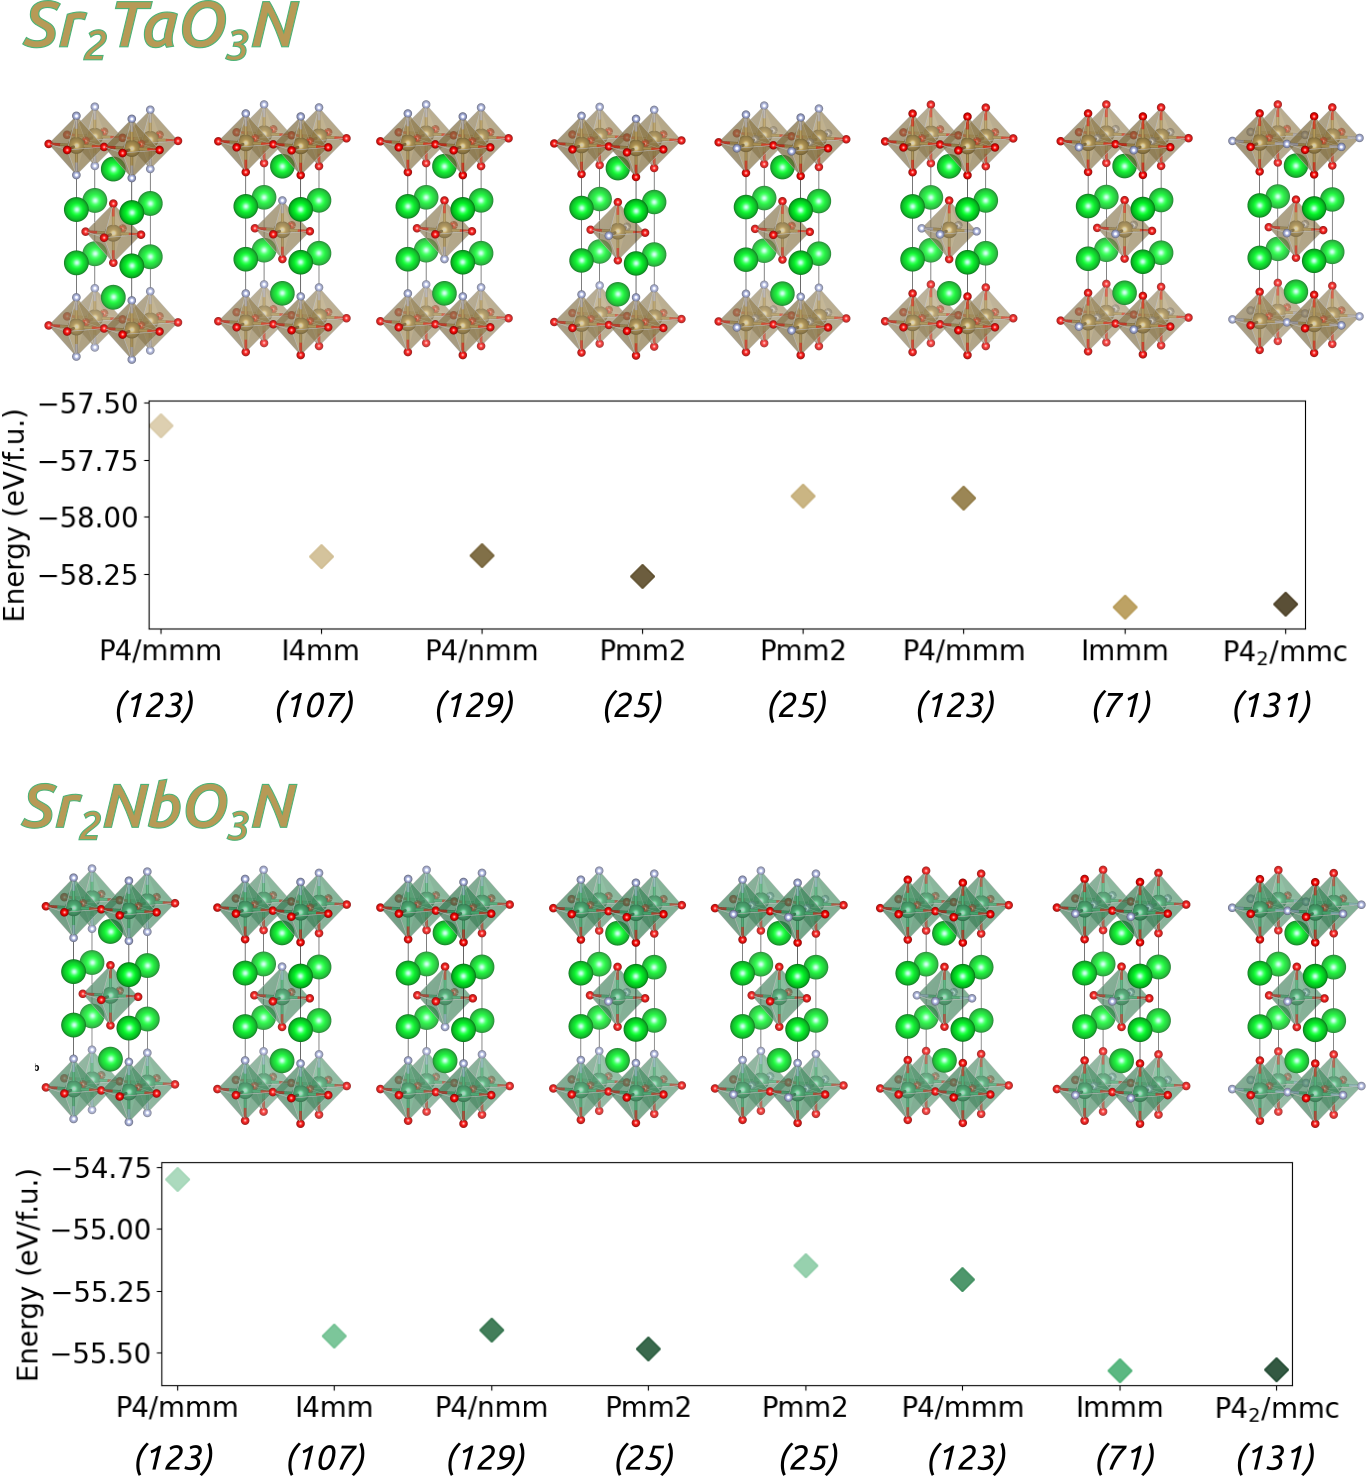
\includegraphics[width=0.9\textwidth]{Figs/rp_ta-nb_e.png}
    \caption{Energía estructural de la concentración $x=1.0$ en función del grupo de simetría espacial para las estructuras Ruddlesden-Popper (arriba) $Sr_{2}TaO_{3}N$ y (abajo) $Sr_{2}NbO_{3}N$.}
    \label{Fig. rp_ta-nb_e}
\end{figure}

Las figuras muestran una diferencia amplia de la energía estructural aportada por \textsc{dft+u} respecto a la energía estructural aportada por \textsc{dft}. Comparando estos resultados calculados con el parámetro \textsc{u} (figura \ref{Fig. rp_ta-nb_energy}) y los resultados sin el parámetro \textsc{u} (figura \ref{Fig. rp_ta-nb_e}): Para el caso de la configuración $Sr_{2}TaO_{3}N$, la energía de cada estructura se ve aumentada en un valor aproximado de $3.25 eV$. Si tomamos un ejemplo para la estructura $Sr_{2}TaO_{3}N$ con grupo de simetría cristalográfico $Immm$(71), la energía sin el parámetro \textsc{u} es de $-58.39eV$, mientras que la energía con el parámetro \textsc{u} es de $-55.15 eV$, es decir existe una diferencia de energía de $-3.24eV$. Para $Sr_{2}NbO_{3}N$, la energía de cada estructura se ve aumentada en un valor aproximado de $3.75 eV$ .Si se hace el mismo análisis para la estructura $Sr_{2}NbO_{3}N$ con grupo de simetría cristalográfico $Immm$(71), la energía sin el parámetro \textsc{u} es de $-55.57 eV$, mientras que la energía con el parámetro \textsc{u} es de $-51.86 eV$, es decir existe una diferencia de energía de $-3.71 eV$. 

Comparando las figuras de energía con y sin \textsc{u} se puede apreciar mas a detalle la diferencia que surge debido a la corrección \textsc{u}. En la figura \ref{Fig. rp_ta-nb_eU} se muestra la comparación de la energía estructural de la fase Ruddlesden-Popper $Sr_{2}(Ta,Nb)O_{4-x}N_{x}$ con y sin el parámetro \textsc{'u'}, tomando en $0.0$ la referencia de la estructura de máxima energía, es decir para las energías calculadas sin el parámetro \textsc{'u'} se toma como referencia la estructura de máxima energía, lo mismo se hace para las energías calculadas con el parámetro \textsc{'u'}.  Ahora quedan barreras de energía reales entre la estructura de mas alta energía y las demás. El hecho de que la energía \textsc{u} afecte mas la configuración con niobio que la configuración con tántalo es debido al tamaño de los átomos. El tántalo es un átomo mas grande, los orbitales están mas lejos, esto hace que entregue los portadores de carga al nitrógeno y al oxigeno mucho mas fácil, pero en el caso de la configuración con niobio, el átomo es mas pequeño, los orbitales están mas cerca del núcleo, esto hace que existan mas problemas de correlación\cite{acgarcia22july}. Los grupos de simetría cristalográficos no cambian respecto a los resultados previos sin el parámetro \textsc{u} debido a que este parámetro  se agrega como una energía en los orbitales y los corrige\cite{acgarcia15july}, mas no afecta las posiciones atómicas.

\begin{figure}[H]
    \centering
    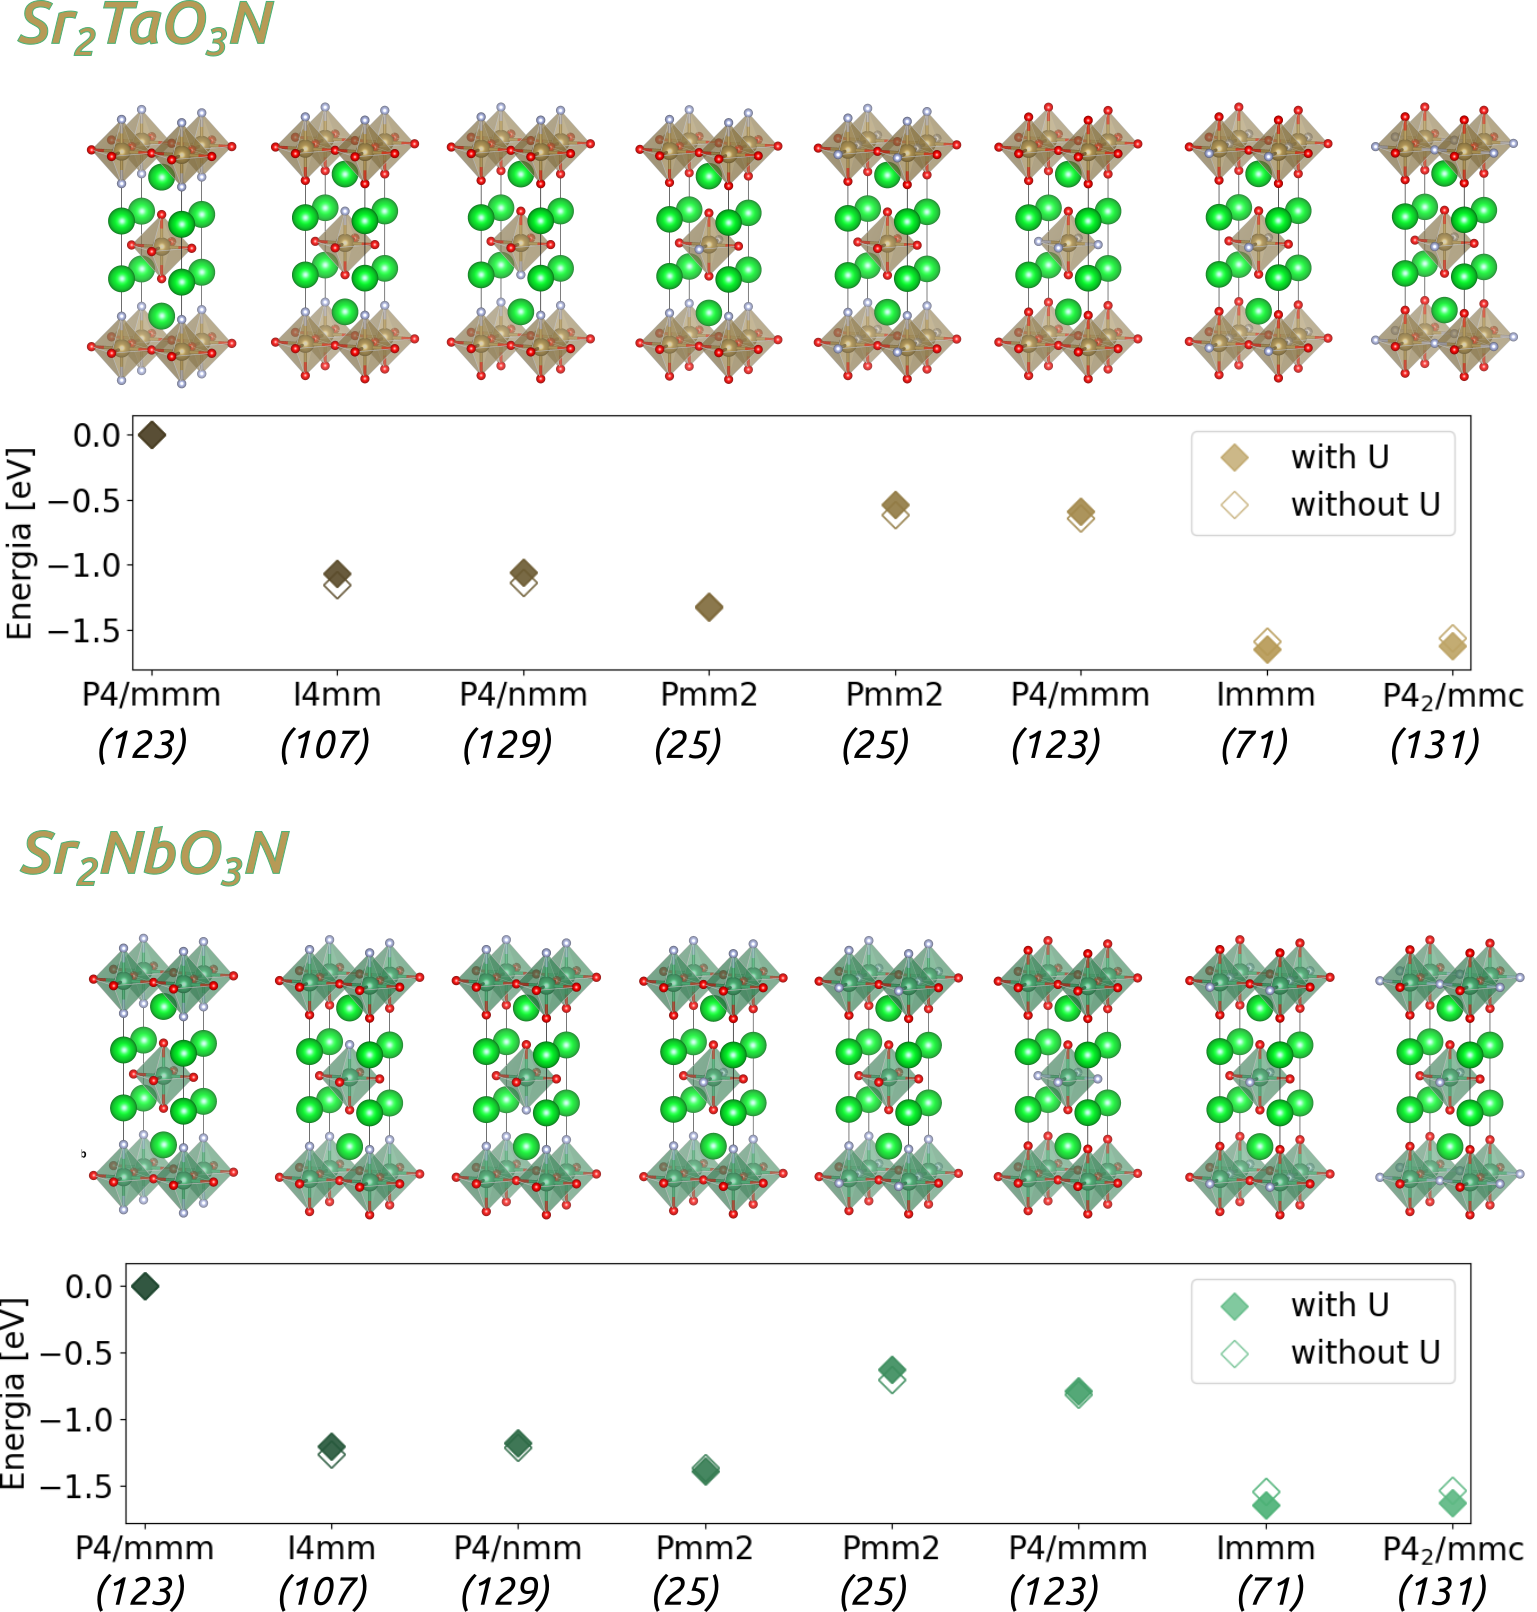
\includegraphics[width=0.9\textwidth]{Figs/rp_ta-nb_eU.png}
    \caption{Energía estructural de la fase Ruddlesden-Popper $Sr_{2}(Ta,Nb)O_{3}N$ en relación a la simetría de grupo espacial a la que corresponde cada estructura.}
    \label{Fig. rp_ta-nb_eU}
\end{figure}







 % Función ode45 de MATLAB
% ------------------------------------------------------------------------
% ------------------------------------------------------------------------
% ------------------------------------------------------------------------
%                                Anexo C
% ------------------------------------------------------------------------
% ------------------------------------------------------------------------
% ------------------------------------------------------------------------
% ------------------------------------------------------------------------
\newpage
\anexo{Grupos de punto polar y enantomórfico}\label{anexoC}
% ------------------------------------------------------------------------
Uno de los mas importantes conceptos en el campo de ciencia de materiales es la simetría, que juega un papel importante en la construcción de propiedades estructurales. En cristalográfica, hay 32 grupos de punto y 230 grupos espaciales que describen las estructuras cristalinas. En especial, la simetría de inversión espacial, la cual indica inmutabilidad bajo inversión de coordenadas espaciales, es de suma importancia en la clasificación de materiales férricos . Entre los 32 grupos de punto , 11 clases centro-simétricas tienen simetría de inversión espacial, mientras que los 21 restantes son no-centro-simétricos \cite{Shi2016SymmetryFerroelectrics}. Los grupos de punto polar que pueden contener ferroelectricidad son: 

\begin{table}[H]
\centering
\begin{tabular}{lrc}
\hline
\multicolumn{1}{c}{\multirow{2}{*}{Sistema cristalino}} & \multicolumn{2}{c}{\multirow{2}{*}{Grupo de punto enantiomórfo}} \\
\multicolumn{1}{c}{}                                    & \multicolumn{2}{c}{}                                             \\ \hline
Triclínico                                              & 1                                       &                        \\
Monoclínico                                             & 2                                       & m                      \\
Ortorómbico                                             &                                         & mm2                    \\
Tetragonal                                              & 4                                       & 4mm                    \\
Trigonal                                                & 3                                       & 3m                     \\
Hexagonal                                               & 6                                       & 6mm                    \\
Cúbico                                                  & \multicolumn{1}{c}{}                    &                        \\ \hline
\end{tabular}
\caption{Grupos de punto polar en cada sistema cristalino en la notación de Hermann-Mauguin \cite{Hermann2015notation}.}
\label{Tab. polar}
\end{table}

Los grupos de puntos que no poseen rotaciones impropias se denominan enantomórficos. Los grupos de punto enantomórfico que pueden contener quiralidad son: 

\begin{table}[H]
\centering
\begin{tabular}{lrc}
\hline
\multicolumn{1}{c}{\multirow{2}{*}{Sistema cristalino}} & \multicolumn{2}{c}{\multirow{2}{*}{Grupo de punto enantiomórfo}} \\
\multicolumn{1}{c}{}                                    & \multicolumn{2}{c}{}                                             \\ \hline
Triclínico                                              & 1                              &                                 \\
Monoclínico                                             & 2                              &                                 \\
Ortorómbico                                             &                                & 222                             \\
Tetragonal                                              & 4                              & 422                             \\
Trigonal                                                & 3                              & 32                              \\
Hexagonal                                               & 6                              & 622                             \\
Cúbico                                                  & 23                             & 432                             \\ \hline
\end{tabular}
\caption{Grupos de punto enantomórfico en cada sistema cristalino en la notación de Hermann-Mauguin \cite{Hermann2015notation}.}
\label{Tab. quiral}
\end{table} % Interfaz de animación de la dinámica del sistema
% ------------------------------------------------------------------------
\bibliography{reference, refweb, referencias}
\appendix

\end{document}                                          % Fin de documento
%